\documentclass[]{book}
\usepackage{lmodern}
\usepackage{amssymb,amsmath}
\usepackage{ifxetex,ifluatex}
\usepackage{fixltx2e} % provides \textsubscript
\ifnum 0\ifxetex 1\fi\ifluatex 1\fi=0 % if pdftex
  \usepackage[T1]{fontenc}
  \usepackage[utf8]{inputenc}
\else % if luatex or xelatex
  \ifxetex
    \usepackage{mathspec}
  \else
    \usepackage{fontspec}
  \fi
  \defaultfontfeatures{Ligatures=TeX,Scale=MatchLowercase}
\fi
% use upquote if available, for straight quotes in verbatim environments
\IfFileExists{upquote.sty}{\usepackage{upquote}}{}
% use microtype if available
\IfFileExists{microtype.sty}{%
\usepackage{microtype}
\UseMicrotypeSet[protrusion]{basicmath} % disable protrusion for tt fonts
}{}
\usepackage[margin=1in]{geometry}
\usepackage{hyperref}
\hypersetup{unicode=true,
            pdftitle={APS 240: Data Analysis and Statistics with R},
            pdfauthor={Dylan Z. Childs},
            pdfborder={0 0 0},
            breaklinks=true}
\urlstyle{same}  % don't use monospace font for urls
\usepackage{natbib}
\bibliographystyle{apalike}
\usepackage{color}
\usepackage{fancyvrb}
\newcommand{\VerbBar}{|}
\newcommand{\VERB}{\Verb[commandchars=\\\{\}]}
\DefineVerbatimEnvironment{Highlighting}{Verbatim}{commandchars=\\\{\}}
% Add ',fontsize=\small' for more characters per line
\usepackage{framed}
\definecolor{shadecolor}{RGB}{248,248,248}
\newenvironment{Shaded}{\begin{snugshade}}{\end{snugshade}}
\newcommand{\KeywordTok}[1]{\textcolor[rgb]{0.13,0.29,0.53}{\textbf{{#1}}}}
\newcommand{\DataTypeTok}[1]{\textcolor[rgb]{0.13,0.29,0.53}{{#1}}}
\newcommand{\DecValTok}[1]{\textcolor[rgb]{0.00,0.00,0.81}{{#1}}}
\newcommand{\BaseNTok}[1]{\textcolor[rgb]{0.00,0.00,0.81}{{#1}}}
\newcommand{\FloatTok}[1]{\textcolor[rgb]{0.00,0.00,0.81}{{#1}}}
\newcommand{\ConstantTok}[1]{\textcolor[rgb]{0.00,0.00,0.00}{{#1}}}
\newcommand{\CharTok}[1]{\textcolor[rgb]{0.31,0.60,0.02}{{#1}}}
\newcommand{\SpecialCharTok}[1]{\textcolor[rgb]{0.00,0.00,0.00}{{#1}}}
\newcommand{\StringTok}[1]{\textcolor[rgb]{0.31,0.60,0.02}{{#1}}}
\newcommand{\VerbatimStringTok}[1]{\textcolor[rgb]{0.31,0.60,0.02}{{#1}}}
\newcommand{\SpecialStringTok}[1]{\textcolor[rgb]{0.31,0.60,0.02}{{#1}}}
\newcommand{\ImportTok}[1]{{#1}}
\newcommand{\CommentTok}[1]{\textcolor[rgb]{0.56,0.35,0.01}{\textit{{#1}}}}
\newcommand{\DocumentationTok}[1]{\textcolor[rgb]{0.56,0.35,0.01}{\textbf{\textit{{#1}}}}}
\newcommand{\AnnotationTok}[1]{\textcolor[rgb]{0.56,0.35,0.01}{\textbf{\textit{{#1}}}}}
\newcommand{\CommentVarTok}[1]{\textcolor[rgb]{0.56,0.35,0.01}{\textbf{\textit{{#1}}}}}
\newcommand{\OtherTok}[1]{\textcolor[rgb]{0.56,0.35,0.01}{{#1}}}
\newcommand{\FunctionTok}[1]{\textcolor[rgb]{0.00,0.00,0.00}{{#1}}}
\newcommand{\VariableTok}[1]{\textcolor[rgb]{0.00,0.00,0.00}{{#1}}}
\newcommand{\ControlFlowTok}[1]{\textcolor[rgb]{0.13,0.29,0.53}{\textbf{{#1}}}}
\newcommand{\OperatorTok}[1]{\textcolor[rgb]{0.81,0.36,0.00}{\textbf{{#1}}}}
\newcommand{\BuiltInTok}[1]{{#1}}
\newcommand{\ExtensionTok}[1]{{#1}}
\newcommand{\PreprocessorTok}[1]{\textcolor[rgb]{0.56,0.35,0.01}{\textit{{#1}}}}
\newcommand{\AttributeTok}[1]{\textcolor[rgb]{0.77,0.63,0.00}{{#1}}}
\newcommand{\RegionMarkerTok}[1]{{#1}}
\newcommand{\InformationTok}[1]{\textcolor[rgb]{0.56,0.35,0.01}{\textbf{\textit{{#1}}}}}
\newcommand{\WarningTok}[1]{\textcolor[rgb]{0.56,0.35,0.01}{\textbf{\textit{{#1}}}}}
\newcommand{\AlertTok}[1]{\textcolor[rgb]{0.94,0.16,0.16}{{#1}}}
\newcommand{\ErrorTok}[1]{\textcolor[rgb]{0.64,0.00,0.00}{\textbf{{#1}}}}
\newcommand{\NormalTok}[1]{{#1}}
\usepackage{longtable,booktabs}
\usepackage{graphicx,grffile}
\makeatletter
\def\maxwidth{\ifdim\Gin@nat@width>\linewidth\linewidth\else\Gin@nat@width\fi}
\def\maxheight{\ifdim\Gin@nat@height>\textheight\textheight\else\Gin@nat@height\fi}
\makeatother
% Scale images if necessary, so that they will not overflow the page
% margins by default, and it is still possible to overwrite the defaults
% using explicit options in \includegraphics[width, height, ...]{}
\setkeys{Gin}{width=\maxwidth,height=\maxheight,keepaspectratio}
\IfFileExists{parskip.sty}{%
\usepackage{parskip}
}{% else
\setlength{\parindent}{0pt}
\setlength{\parskip}{6pt plus 2pt minus 1pt}
}
\setlength{\emergencystretch}{3em}  % prevent overfull lines
\providecommand{\tightlist}{%
  \setlength{\itemsep}{0pt}\setlength{\parskip}{0pt}}
\setcounter{secnumdepth}{5}
% Redefines (sub)paragraphs to behave more like sections
\ifx\paragraph\undefined\else
\let\oldparagraph\paragraph
\renewcommand{\paragraph}[1]{\oldparagraph{#1}\mbox{}}
\fi
\ifx\subparagraph\undefined\else
\let\oldsubparagraph\subparagraph
\renewcommand{\subparagraph}[1]{\oldsubparagraph{#1}\mbox{}}
\fi
\usepackage{booktabs}

%%% Use protect on footnotes to avoid problems with footnotes in titles
\let\rmarkdownfootnote\footnote%
\def\footnote{\protect\rmarkdownfootnote}

%%% Change title format to be more compact
\usepackage{titling}

% Create subtitle command for use in maketitle
\newcommand{\subtitle}[1]{
  \posttitle{
    \begin{center}\large#1\end{center}
    }
}

\setlength{\droptitle}{-2em}
  \title{APS 240: Data Analysis and Statistics with R}
  \pretitle{\vspace{\droptitle}\centering\huge}
  \posttitle{\par}
  \author{Dylan Z. Childs}
  \preauthor{\centering\large\emph}
  \postauthor{\par}
  \predate{\centering\large\emph}
  \postdate{\par}
  \date{2016-10-11}

\begin{document}
\maketitle

{
\setcounter{tocdepth}{1}
\tableofcontents
}
\chapter{Course information and
overview}\label{course-information-and-overview}

This is the online course book for the \textbf{Data Analysis and
Statistics with R}
(\href{https://www.shef.ac.uk/aps/currentug/level2/aps240}{APS 240})
module. You can view this book in any modern desktop browser, as well as
on your phone or tablet device. The site is self-contained---it contains
all the material you are expected to learn this year.

\href{https://www.shef.ac.uk/aps/staff-and-students/acadstaff/childs}{Dylan
Childs} is the course co-coordinator. Please
\href{mailto:d.childs@sheffield.ac.uk?Subject=APS\%20133\%20general\%20query}{email
him} if you have have any general queries about the course.
\href{https://www.shef.ac.uk/aps/staff-and-students/acadstaff/beckerman}{Andrew
Beckerman} is the second course instructor. The Teaching Assistants
(`TAs') this year are Ross Booton, Matthew Hethcoat, Bethan Hindle,
Tamora James, Felix Lim, and Simon Mills.

\section{Why do a data analysis course?}\label{why-data-analysis}

To do science yourself, or to understand the science other people do,
you need some understanding of the principles of experimental design,
data collection, data presentation and data analysis. That doesn't mean
becoming a maths wizard, or a computer genius. It means knowing how to
take sensible decisions about designing studies and collecting data, and
then being able to interpret those data correctly. Sometimes the methods
required are extremely simple, sometimes more complex. You aren't
expected to get to grips with all of them, but what we hope to do in the
course is to give you a good practical grasp of the core techniques that
are widely used in biology and environmental sciences. You should then
be equipped to use these techniques intelligently and, equally
importantly, know when they are not appropriate, and when you need to
seek help to find the correct way to design or analyse your study.

You should, with some work on your part, acquire a set of skills which
you will use at various stages throughout the remainder of your course,
in practicals, field courses and in your project work. These same skills
will almost certainly also be useful after your degree, whether doing
biology, or something completely different. We live in a world that is
increasingly flooded with data, and people who know how to make sense of
this are in high demand. The R statistical programming environment
underpins much of this endeavour, in both academic and commercial
settings. Learning the basic principles of data analysis with R will
only improve your employment prospects.

\section{Course overview}\label{overview}

\subsection{Aims}\label{aims}

This course has two main, and equal, aims. The first is to provide a
basic training in the use of statistical methods and software (R and
RStudio) to analyse biological data. The second is to introduce some of
the principles of experimental design, sampling, data interpretation,
graphical presentation and scientific writing relevant to the biological
and environmental sciences.

\subsection{Objectives}\label{objectives}

By the end of the course you should be familiar with the principles and
use of a range of basic statistical techniques, be able to use the R
programming language to carry out appropriate analyses of biological
data, evaluate your statistical models, and make sensible interpretation
of the results. You should be able to relate the ways in which data are
collected (by different designs of sampling or experiment) to the types
of statistical methods that can be used to analyse those data. In
combination with the skills you developed in
\href{https://www.shef.ac.uk/aps/currentug/level1/aps135}{APS 135}, you
should be able to decide on appropriate ways of investigate data
graphically, be able to produce good quality scientific figures, and
incorporate these, along with statistical results, into a formal report.

\subsection{Assumed background}\label{assumed-background}

You are assumed to be familiar with the use of personal computers on the
University network, and with the use of R for data input, manipulation
and plotting introduced in
\href{https://www.shef.ac.uk/aps/currentug/level1/aps135}{APS 135}. If
you are unsure about these basic methods, then you will need to revise
the material covered in the Level 1 IT practicals. The key skills you
need are covered in the
\protect\hyperlink{programming-prerequisites}{Programming prerequisites}
chapter. We will revise the most important topics in the first practical
session.

\begin{do-something}
\textbf{Environmental Sciences Students}

Don't panic if you are one of the Environmental Sciences students
joining us from Geography. We'll provide targetted help at the beginning
of the course to help you learn the fundamentals of R.
\end{do-something}

\subsection{Methods}\label{methods}

The course runs over semester 1, in weeks 1-12. The first 10 weeks
consists of a 2-hour IT practical each week, along with some additional
preparatory practical work and reading. All components of the course are
compulsory. The remaining 2 weeks are devoted to revision and an
assessed data analysis project.

Students come to APS 240 with very different experiences and
competancies. Because of this unavoidable situation, the course is
designed as a `self-teaching' module to you flexibility in the rate at
which you work through the material. This doesn't mean no one is going
to help you, but you are expected to take responsibility of your own
learning.

\subsubsection{Preparatory reading and practical
work}\label{preparatory-reading-and-practical-work}

Each week starts with some preparatory reading and `walk-through'
practical work from the course book. We'll let you know what you need to
do each week. The book chapters generally come in one of two forms:

\begin{itemize}
\item
  \textbf{Practical walk-through chapters.} These are designed to
  introduce the practical aspects of different analysis techniques.
  These generally focus on the `when' and `why' we use a particular
  technique, as well how to actually do it in R. You are free
  (encouraged even) to work through these in groups.
\item
  \textbf{Concept chapters.} These focus on ideas and concepts, rather
  then using R \emph{per se} (though they may use R from time to time).
  They provide background information or more detailed discussion
  relating to the topics you are covering. These are an integral part of
  the course. Please don't skip them!
\end{itemize}

It is up to you to complete the preparatory work in your own time.
However, we are not expecting you to understand everything the first
time around. This point is so important it's worth saying again---you
are not expected to understand everything in the course book the first
time you read it. Just do your best to understand it, taking careful
notes of anything you're struggling with. The TAs and staff will happily
answer any questions you have during the timetabled sessions. Indeed,
that is what they're there to do.

\subsubsection{Timetabled practicals}\label{timetabled-practicals}

The \textbf{timetabled practicals} take place in the APS IT rooms,
either Perak IT labs or B56. In each of these sessions, you will work
through a number of small exercises to help you consolidate what you're
been working on. You'll be asked to note down your answers to some of
the exercises. The correct answers will be available. TAs and staff are
there to help if you get stuck, so don't suffer in silence. You can
(should!) also use this time to ask questions about concepts that are
confusing you.

You are welcome to use your own computer to complete your work. Keep in
mind that the university computers are the only `officially supported'
platform. If you run into a problem using your own computer, the TAs and
staff will try to help resolve these. Unfortunately, if these prove to
be intractable, you will have to use the university computing
facilities. It just isn't fair on other students for teaching staff to
spend valuable contact time trying to solve installation / setup
problems.

\subsection{Non-assessed material}\label{non-assessed-material}

Although every topic is important, in the sense that it contains
material that will help you become a better data analyst, we want to
avoid creating too much of an assessment burden in this course. To this
end, the material in a few of the chapters is be formally assessed. The
\protect\hyperlink{expected-learning-outcomes}{Expected learning
outcomes} chapter tells you what you need to be able to know by the end
of the course. If you're the kind of person who wants to focus on the
assessment, you should use that as your guide. As always, feel free ask
an instructor (not a TA) for clarification if you're not sure of what
you need to be able to do.

\subsection{What is required of you?}\label{what-is-required-of-you}

A willingness to learn and to take responsibility for your learning!
Data analysis is not the easiest subject in the world, but neither is it
the most difficult. It's worth making the effort. What you learn in this
course will form the basis for much of what you do in field course,
practical and project work that follows in later semesters.

The minimum requirement for the course is that you:

\begin{itemize}
\item
  attend your designated practical session each week (please ensure that
  you arrive on time and register, or you will be recorded as absent),
\item
  complete the preparatory practical work and reading, taking careful
  notes of anything that you don't understand,
\item
  be proactive about your lerning and ask the TAs and staff questions
  about things you're struggling with,
\item
  complete the exercises for each week before the next practical class,
  and check through your answers to questions using MOLE.
\end{itemize}

How you work through the book is fairly flexible, but remember, the
self-study preparatory work lays the foundatation for the material
covered in the timetabled practicals. Take our word for it, you won't
get much out of the timetabled sessions if you skip the preparatory
work.

In each practical session you should aim to complete most, if not all,
of the exercises for that practical. If you don't manage to do this you
should try to finish off the work in your own time before the next
practical. However, if you have problems with any of the work, staff
will help you during the practical sessions, even if it is not the topic
designated for that session. So if you need to catch up, there will be
opportunities to do so.

A word of advice: Don't let the flexibility of the course tempt you into
letting a backlog of work build up. This will compromise your ability to
do the assessed work when it is set and will make it difficult to revise
for the exam.

One last point: \textbf{the university guidelines assume the total study
time associated with a 10 credit module to be about 100 hours}. There is
an expectation that you will spend significant time outside the
timetabled practical classes working on this module. You should aim to
spend about 5 hours each week working through the chapters, completing
the practical exercises, and finally, working on the assessed project.
This leaves you about 40 hours to revise for the formal exam in the new
year.

\subsection{Assessment}\label{assessment}

Assessment of the course will have two components. The first is a short
data analysis project in weeks 11-12 of the course, the second is an
open book exam in the winter exam period. `Open book' means you will
have access to this book during the exam, i.e.~you don't have to
memorise everything in here, just understand it!

Further details will be given as the course progresses.

\section{How to use the teaching
material}\label{how-to-use-the-teaching-material}

\subsection{The online course book}\label{printed-material}

All of the teaching material will be made available through a single
online course book (this website). The book is organised such that it
forms a complete, stand-alone introduction to data analysis. You should
bookmark this now if you haven't already done so. There are a couple of
very good reasons for delivering the course material this way:

\begin{itemize}
\item
  \textbf{Practicality}: Most exercises can be completed by building on
  the examples in the course material. Copying the relevant R code from
  the course website and pasting it into your script is much more
  efficient, and less error-prone, than copying by eye from a printed
  page. A website also allows us to cross-reference topics and link to
  the odd bit of outside reading.
\item
  \textbf{Permanence}: Experience suggests that many of you will want to
  refer to the material in this course after you graduate. However, bits
  of paper are easy to lose, and because the R landscape is always
  changing, some elements of the course may be less relevant in a few
  years time. By putting everything on a website, we can ensure that you
  will always be able to access a familiar, but up-to-date data analysis
  course.
\end{itemize}

\subsection{Printed material}\label{printed-material}

There is a small amount of printed material in this course:

\begin{itemize}
\item
  \textbf{Cheat sheets}: We will supply you with copies of the
  \texttt{dplyr} and \texttt{ggplot2}
  \href{https://www.rstudio.com/resources/cheatsheets/}{cheat sheets}
  produced by the people who build RStudio . It may help you to refer to
  these when you need use either the \texttt{dplyr} or \texttt{ggplot2}
  packages in a practical.
\item
  \textbf{Assessment information}: Although much of the assessment will
  be done on the computer, any information relating to the assessments
  will be produced in printed form. This will be handed out in week 10.
\end{itemize}

\subsection{How to make best use of the teaching
material}\label{how-to-make-best-use-of-it}

DO:

\begin{itemize}
\item
  When working through an exercise, follow the instructions carefully,
  but also \textbf{think about what you are doing}. Work at your own
  pace; you are not being assessed on whether you can do an exercise in
  a particular time.
\item
  Ask teaching staff for help in the practicals if there are things that
  you don't follow, or when things don't seem to come out the way they
  should---that's what they're there for!
\item
  Collaborate! If you are not sure you understand something feel free to
  discuss it with a friend---more often than not this is exactly how
  scientists resolve and clarify problems in their experimental design
  and analysis.
\item
  Be prepared to experiment with R to solve problems that you encounter.
  You can't break your R or RStudio by generating errors. When you run
  into a problem, go back to the line of code that generated the first
  error and try making a change.
\item
  Complete each week's work before the next week's session. You may be
  able to complete some sessions quite quickly, others may take more
  time and require more work on your own outside the timetabled periods.
\end{itemize}

DON'T:

\begin{itemize}
\item
  Just copy what someone else tells you to do without understanding why
  you are doing it. You need to understand it for yourself (and you'll
  be on your own in the exam).
\item
  Skip practicals or preparatory work and get behind schedule --- there
  is too much material to assimilate all at once when you get to the
  assessments. Like all skills data analysis is something you have
  practice.
\end{itemize}

\subsection{Conventions used in the course material}\label{conventions}

The teaching material, as far as possible, uses a standard set of
conventions to differentiate between various sorts of information,
action and instruction:

\subsubsection{Text, instructions, and
explanations}\label{text-instructions-and-explanations}

Normal text, instructions, explanations etc. are written in the same
type as this paragarph (obvious really), we will tend to use bold to
highlight specific technical terms when they are first introduced.
Italics are generally used for emphasis and with Latin names.

When we want you to do something important or pay particular
attentions---e.g., waksing you to write down an answer or giving you a
set of instructions---we place the text inside a box like this one:

\begin{do-something}
\textbf{Brown boxes}

Here is some important text telling you to do something or remember
something important. Sometimes it just contains a warning that the next
bit will be hard\ldots{}
\end{do-something}

Please don't ignore these. At various points in the text you will also
come across different coloured boxes that contain additional
information:

\begin{advanced-box}
\textbf{Blue boxes}

These aim to offer a not-too-technical discussion of how or why
something works the way it does. These are things that it may be useful
to know, or at least know about, but aren't necessarily part of the main
thread of a section.
\end{advanced-box}

\begin{warning-box}
\textbf{Red boxes}

These contain a \textbf{warning} or flag a common \textbf{gotcha} that
may trip you up. They highlight potential pitfalls and show you how to
avoid them. You will avoid a lot of future mistakes if pay close
attention to these.
\end{warning-box}

We use block quotations to indicate an example of how a particular
statistical result should be presented when you write it in a report:
e.g.

\begin{quote}
The mean lengths of male and female locusts differed significantly
(t=4.04, df=15, p=0.001), with males being significantly larger.
\end{quote}

\subsubsection{R code, files and
RStudio}\label{r-code-files-and-rstudio}

\texttt{This\ typeface} is used to distinguish R code within a sentence
of text: e.g. ``We use the \texttt{summary} function to obtain
information about an object produced by the \texttt{lm} function.''

A sequence of selections from an RStudio menu is indicated as follows:
e.g. \textbf{File ▶ New File ▶ R Script}

File names referred to in general text are given in upper case in the
normal typeface: e.g.~MYFILE.CSV.

\subsection{Feedback}\label{feedback}

There are a number of ways in which you can obtain feedback on how well
you understand the course material

\subsubsection{Self-assessment
questions:}\label{self-assessment-questions}

At various points in the course material there are questions for you to
answer. When you reach one of these, you should be in a position to
answer the question ---- so make a note of the answer! When you've
completed the session, you can check your answers using the `self-test'
for that particular session on MOLE. You will see if you have the
correct answer and in some cases you will also get some additional
explanation as to why that answer is right (or wrong!).

\subsubsection{Each other:}\label{each-other}

Discussing what you are doing with someone as you go along, or working
through a problem with someone else, can help clarify your
understanding. Please bear in mind, however, that you learn little or
nothing by simply copying information from someone else, and when it
comes to the assessed project, it must be your own work.

\subsubsection{Staff:}\label{staff}

In the practicals you will have opportunities to ask questions and
discuss what you are doing with staff and teaching assistants. They are
not just there to help you with the practical. You should use them to
help you work through any problems you have with the course material,
both conceptual and practical. There will also be an opportunity to have
topics you raise discussed in later practicals.

\subsection{Help sessions}\label{help}

We will run an open `help' session every Friday from 12-2.00pm, in the
B56 IT Room in APS. An instructor will be on hand during this period to
answer specific questions about the course material. This room holds
about 40 students, so please only attend if you require one-to-one
assistance, i.e, don't just use this session to complete unfinished
practicals (unless you are stuck of course).

\subsection{Overall\ldots{}}\label{overall}

We hope that the material is clear and easy to use, and that you find
the course useful, or even enjoy it!

In a text of this size, which is continually being improved and updated,
errors do creep in; if you find something you think is wrong please tell
us. If it's not wrong we will be happy to explain why, and if it is then
you will save yourself and others a lot of confusion. Similarly, if you
have any comments or suggestions for improving the teaching materials
please let us know.

\section{Health and safety using display screen
equipment}\label{health-and-safety}

Although using a computer may not seem like a particularly risky
activity you should be aware that you can suffer ill effects if you work
at a computer for long periods without observing a few sensible
precautions. The standard guidelines are as follows:

\begin{itemize}
\item
  Make sure that your equipment is properly adjusted:

  \begin{itemize}
  \item
    ensure that your lower back is well supported by adjusting the seat
    back height
  \item
    adjust your chair seat height so that your forearms are level when
    using the keyboard
  \item
    make sure that the front edge of the keyboard is at least 8-10 cm
    away from the edge of the desk
  \item
    if you are using a mouse, have it far enough away from the edge of
    the desk so that your wrist is supported whilst you use it. If you
    can learn to use the mouse with either hand then this can help avoid
    strains
  \end{itemize}
\item
  Do not have your screen positioned in such a way that there is glare
  or reflections from the windows or room lights on the screen.
\item
  Maintain good posture.
\item
  Take regular breaks away from the computer. It is recommended that you
  take about 10 minutes break every hour.
\end{itemize}

Most Departments will have a Display Screen Trainer or Advisor, who can
offer specific advice if you are using a display screen for a
substantial amount of time, or if you experience, or anticipate,
specific problems.

\hypertarget{expected-learning-outcomes}{\chapter{Expected learning
outcomes}\label{expected-learning-outcomes}}

\section{Statistical Concepts (I)}\label{statistical-concepts-i}

\begin{itemize}
\item
  Given a description of some data, classify variables as numeric vs
  categorical, ratio vs.~interval, and ordinal vs.~nominal.
\item
  Construct simple summaries of numeric variables in R using the
  \texttt{mean}, \texttt{sd}, \texttt{var} functions.
\item
  Explain what sampling error is (in non-technical terms) and understand
  why it is necessary to quantify sampling error alongside point
  estimates.
\item
  Recognise the difference between the distribution of a sample, and the
  sampling distribution of an estimate derived from that sample.
\item
  Recognise the difference between the standard deviation (a property of
  a sample) and the standard error (a property of a sampling
  distribution).
\item
  Calculate the standard error of a sample mean when the population
  distribution of a variable follows a normal distribution.
\item
  Given a description of an experimental setting, be able to
  recognise\ldots{}

  \begin{enumerate}
  \def\labelenumi{\arabic{enumi}.}
  \tightlist
  \item
    \ldots{}the difference between a statistical population and a sample
    from the population.
  \item
    \ldots{}the difference between a population parameter and a point
    estimate of the population parameter.
  \end{enumerate}
\end{itemize}

You are not expected to be able to explain or use the bootstrap or
permutation tests---these were introduced to help you learn the
principles listed above.

\hypertarget{programming-prerequisites}{\chapter{Programming
prerequisites}\label{programming-prerequisites}}

This chapter gives a quick overview of the prerequisite R skills needed
for this course (we studied these last year). We will use these skills
this year, so you may need to spend revising them if you feel that
you're a little rusty.

\begin{do-something}
\textbf{Biology students}

The key R skills you need to have in place to work through this book
will be revised in the first practical session. The lecture slides will
be placed on MOLE after the practical. You can also access a version
without the answers to exercises
\href{./presentations/revision_lecture_students.html}{here}.

\textbf{Environmental Science students}

If you are an Environmental Science student joining us from Geography
the material in this section won't make any sense to you at the moment.
Don't panic! We will help you catch up in the first few weeks of the
course, and because you will be working in a smaller group, you will be
able to access more one-to-one help.
\end{do-something}

\section{Starting an R session in
RStudio}\label{starting-an-r-session-in-rstudio}

Here is a quick overview of the process you should go through every time
you start a new R session:

\begin{enumerate}
\def\labelenumi{\arabic{enumi}.}
\item
  Open up RStudio and set your working directory. You should do this via
  the RStudio menu system: \textbf{Session ▶ Set Working Directory ▶
  Choose Working Directory\ldots{}}. Make sure that you choose a
  sensible location. This is where you will store your data and R
  scripts, so it needs to be somewhere you can find and access again
  each time you use R. If you want to keep life really simple, it is a
  good idea to use the same location in every practical, but you don't
  have to do this.
\item
  Open up a new R script using the RStudio menu system: \textbf{File ▶
  New File ▶ R Script}. Don't create any other kind of file.
\item
  There are a couple of things that need appear at the start of every
  script. Add these to the top of your new script before you do anything
  else. You should always clear the workspace with \texttt{rm}, and load
  up any packages you plan to use:
\end{enumerate}

\begin{Shaded}
\begin{Highlighting}[]
\CommentTok{# clear the workspace so that we have a 'clean sheet'}
\KeywordTok{rm}\NormalTok{(}\DataTypeTok{list =} \KeywordTok{ls}\NormalTok{())}

\CommentTok{# load and attach the packages we want to use...}
\CommentTok{# 1. 'dplyr' for data manipulation}
\KeywordTok{library}\NormalTok{(dplyr)}
\CommentTok{# 2. 'ggplot2' for plotting}
\KeywordTok{library}\NormalTok{(ggplot2)}
\end{Highlighting}
\end{Shaded}

\begin{enumerate}
\def\labelenumi{\arabic{enumi}.}
\setcounter{enumi}{3}
\item
  Now run the preamble section of the script, i.e.~highlight everything
  and hit \textbf{Ctrl+Enter}. If the \texttt{library} commands didn't
  work it suggests that you have not previously installed the relevant
  package. Install the package (see below) and try rerunning the script.
\item
  Once the preamble bit of the script is working you should save the
  script. Look at the label of the tab the script lives in. This will
  probably be called something like \emph{Untitled1}, and it the label
  will be red. This is RStudio telling you that you have not saved the
  file yet.
\end{enumerate}

You are now ready to start developing your new script.

\section{Using packages}\label{using-packages}

R packages extend the basic functionality of R so that you can do more
with it. A package bundles together R code, data, and documentation in a
way that is easy to use and share with other users. Last year we learned
how to use some of the functions provided by the \texttt{dplyr} package
(for data manipulation) and the \texttt{ggplot2} package (for making
plots). We are going to use the \texttt{dplyr} and \texttt{ggplot2}
packages again this year, so you need to understand R's package system
in order to access these. You can revise how to use the package system
in the
\href{http://dzchilds.github.io/aps-data-analysis-L1/help-packages.html}{packages}
topic. It isn't difficult to use, and we will obviously help you if you
run into difficulties.

Installing a package is done via the \texttt{install.packages} function,
e.g.

\begin{Shaded}
\begin{Highlighting}[]
\KeywordTok{install.packages}\NormalTok{(}\StringTok{"dplyr"}\NormalTok{)}
\end{Highlighting}
\end{Shaded}

Loading and attaching the package a package happens via the
\texttt{library} function, e.g.

\begin{Shaded}
\begin{Highlighting}[]
\KeywordTok{library}\NormalTok{(}\StringTok{"dplyr"}\NormalTok{)}
\end{Highlighting}
\end{Shaded}

The key point---which seems to cause endless confusion---is that
installing a package, and then loading and attaching the package, are
different activities. You only have to install it once onto your
computer, but you have to load a package every time you want to use it
in a new R session (i.e.~every time you start up RStudio).

\section{Reading data into R}\label{reading-data-into-r}

Last year we made extensive use of several data sets that reside inside
various R packages. This was useful because it meant we could use the
data without first reading it into R, meaning that we could concentrate
on developing your R skills rather than fixing data input errors. We
don't have the luxury of doing this when we work with our own data, and
so this year, we will adopt more realistic practices. Whenever you need
to work with a data set, you will have to first download it (from MOLE),
and then read it into R. Each data set is stored as a Comma Separated
Value (`CSV') text file, and so you will need to use the
\texttt{read.csv} function to read it in. You can revise how all of this
works in the relevant section of the
\href{\%7B\%7Bsite.baseurl-L1\%7D\%7D/data-frames.html\#access-data}{data
frames} topic.

\section{Data frames}\label{data-frames}

When you read data into R using a function like \texttt{read.csv}, it
places that data into a data frame. The data frame is the most important
type of object in R. It is table-like object that collects together
different variables, storing each of them as a named column. We can
access the data inside a data frame by referring to particular columns
and rows. You can revise how to work with data frames in the
\href{\%7B\%7Bsite.baseurl-L1\%7D\%7D/data-frames.html\#access-data}{data
frames} topic.

\section{Package functions}\label{package-functions}

We will use functions from the \texttt{dplyr} package from time-to-time
to manipulate data, and we will use the \texttt{ggplot2} package to make
plots of our data and summarise statistical models. However, we will
remind you which functions you need to use to solve a particular problem
as the course unfolds, so there is no need to revise all of this
material now.

\part{Statistical Concepts
(I)}\label{part-statistical-concepts-i}
\addcontentsline{toc}{chapter}{(PART) Statistical Concepts (I)}

\hypertarget{the-scientific-process}{\chapter{The scientific
process}\label{the-scientific-process}}

\begin{quote}
\emph{There is something fascinating about science. One gets such a
wholesale return of conjecture out of a trifling investment of fact.}

Mark Twain

\emph{To do science is to search for patterns, not simply to accumulate
facts.}

Robert MacArthur
\end{quote}

\section{Stages in the scientific
process}\label{stages-scientific-process}

Science is about asking, and answering, the right questions. Within this
process a number of distinct stages usually occur: making observations,
asking questions, formulating hypotheses, and testing predictions.
Collectively these are the building blocks of what is known as the
scientific method. Exactly how they fit together, and what the
philosophical and practical limitations of different approaches are,
have been the subject of much debate by philosophers of science. We are
not going to tackle those issues here, fascinating though they are, but
instead try to extract a general working framework for the process of a
typical scientific investigation.

\subsection{Observations}\label{stages-observations}

\textbf{Observation} --- \emph{information, or impression, about events
or objects}.

In general the questions we ask are not generated by pure abstract
thought, but are a result of observations about the natural world. These
may take the form of direct observations we make ourselves, patterns
that crop up in data collected for other purposes, in non-specific
surveys, and the previous work, or accumulated information, of other
people.

So, while pottering around in a stream one day, you notice that the
freshwater `shrimps' (\emph{Gammarus}) that abound in the stream seem to
occur almost entirely under stones; you rarely seem to see them when you
just watch a patch of open stream bed. Having made observations, it may
be necessary to collect some more data to check that this phenomenon is
not just a one-off event, or a false impression. Look under a few more
stones, watch the same species another day, or in another place, check
the literature for similar observations by others.

Such observations of biological systems will lead almost automatically
into asking questions.

\subsection{Questions}\label{stages-questions}

\textbf{Question} --- \emph{what it is that you want to know; the scope
of your investigation}.

e.g., Why does \emph{Gammarus} spend most of its time under stones?

You should try and make your question reasonably focused - the overall
aim of your study is to answer this question. The question of why the
tropics are more diverse than the temperate regions is a vast topic - so
even though it is a valid (and fascinating) question, it may not be a
good choice for a final year project or even a PhD!

The next stage is to formulate an hypothesis.

\hypertarget{stages-hypotheses}{\subsection{Hypotheses}\label{stages-hypotheses}}

\textbf{Hypothesis} --- \emph{an explanation proposed to account for
observed facts.}

In general, in biology, the important distinguishing feature of an
hypothesis is that it specifies some biological process, or processes,
which might account for the observations made. One question will often
generate more than one hypothesis:

\emph{Gammarus} occur under stones because:

\begin{itemize}
\item
  they need to shelter from the current
\item
  their food (leaf litter) gets trapped and accumulates under stones
\item
  they are subject to predation by visually hunting fish and need to
  remain out of sight
\end{itemize}

Formulating hypotheses requires more than just a restatement of the
question - it usually embodies some mechanism (though in some cases this
may not be fully understood) and it will often draw on additional
information (e.g., the fact that \emph{Gammarus} feed on dead leaves).

\subsection{Predictions}\label{stages-predictions}

\textbf{Prediction} --- \emph{what you would expect to see if the
hypothesis was true}.

Hypotheses are about proposing explanations, but they might not be
directly testable; that is they may not tell you what data to collect,
or what pattern to expect in the data. To be able to test an hypothesis
you need to make some predictions from that hypothesis. These will be
determined both by what you expect to see and what it is possible, or
practical, to measure. A prediction is not simply a rephrasing of the
hypothesis - it should more or less give you a statement of the
experiment to conduct or observation to make, and type of data to
collect:

\begin{itemize}
\item
  \emph{Shelter hypothesis:} a greater proportion of \emph{Gammarus}
  should be found in the open in streams with slow flow, or in slower
  flowing areas of a stream.
\item
  \emph{Food hypothesis:} \emph{Gammarus} should not aggregate under
  stones from which all leaf litter has been removed; \emph{Gammarus}
  should aggregate on patches of leaf litter tethered in the open part
  of the stream bed.
\item
  \emph{Predation hypothesis:} \emph{Gammarus} should aggregate under
  stones more in streams where fish are present than where they are not;
  \emph{Gammarus} may spend less time under stones at night.
\end{itemize}

Ideally you are looking for a prediction that is unique to the
hypothesis it is based on - so if the prediction is true only one of the
hypotheses could have been responsible, but this may not always be
possible and some combination of predictions may need to be used.
Additionally, several processes may be operating at the same time. This
makes hypothesis testing harder still. It may be necessary to consider
two or more hypotheses, and their corresponding predictions, in
combination. For example, \emph{Gammarus} may be under stones because it
prefers the sheltered environment, but also because food accumulates
there. In this case we might expect that \emph{Gammarus} will show a
weak aggregative response to shelter alone, or food alone, and a
stronger one to them both together.

\section{Hypothesis testing}\label{hypothesis-testing}

Once we have firmed up our questions, hypotheses, and predictions we can
collect the data to evaluate our ideas. On the basis of these data we
will either accept or reject the various hypotheses. The important thing
to realise about the process of hypothesis testing is that, in science
especially, hypotheses are either rejected, or not rejected, but an
hypothesis can rarely, except in trivial cases, be proved.

This seems like an odd state of affairs! True, but it does make sense.
Since you cannot be sure that you have thought of all the possible
hypotheses to explain an observation, finding evidence that supports the
prediction from one of your hypotheses, does not guarantee that the
hypothesis is the only one which could have produced the effect you
find. On the other hand, if you find evidence that directly contradicts
the prediction(s) from your hypothesis, you can be certain (assuming the
prediction and data are not flawed) that the hypothesis cannot be true.

An hypothesis which predicted that all conifers should be evergreen
could be supported by numerous observations of different conifer species
in forests around the world, but is conclusively refuted by the first
larch tree we encounter.

Having tested your hypothesis, by examining the evidence that its
predictions are true, you may accept it as the best (so far) explanation
of the observations, or you may reject it as an explanation, and turn to
other hypotheses. The same procedure must then be repeated for these
hypotheses.

This basic cycle of proposing hypotheses and then seeking evidence
potentially capable of falsifying them, is, in essence, the idealized
model of the scientific process famously proposed by the philosopher of
science Karl Popper (1902-1994). It is often termed
\emph{falsificationism}.

\section{Don't we ever know anything for sure?}\label{are-we-sure}

The method presented here provides a view of science as one in which we
suggest hypotheses, then test them, trying to reject them by finding
conclusive counter-evidence, then replacing them with new hypotheses. It
all sounds a bit frustrating. In fact of course we do `accept'
hypotheses all the time --- that is we fail to reject them over and over
again. These hypotheses become more accepted and in some sense become
regarded as `true' if repeated attempts to test them all fail to provide
good counter evidence. In other words, we have some ideas that are doing
pretty well in terms of resisting falsification, and we use these as our
best estimates of the truth, with the proviso that it is still possible
a better idea will come along in due course.

The simple process of falsification described above also presents a
picture of scientists as wonderfully neutral, objective creatures,
rationally proceeding through cycles of setting up hypotheses, testing
them, rejecting them, cheerfully setting them aside and starting over
again. Of course this is not a true reflection of the complex, often
messy, business really involved in trying to figure out how the world
works. Philosophers of science have argued long and hard about how far
from this idealized process real science actually is. Various
alternative philosophies suggest more `realistic' processes, such as
Thomas Kuhn's view of science as periods of relative stasis, where
people work within an accepted paradigm (a set of views about how things
work) despite accumulating evidence that doesn't always support the
paradigm, until finally it is upset by a `revolution' which rejects the
entire paradigm, and proposes a new view. The philosopher Imre Lakatos
proposed some resolution of these views, suggesting that scientific
ideas were grouped together in `research programmes' concerned with
particular endeavours, and that within these there may be core ideas
that are not challenged, but other related ideas which are being
challenged and adjusted by falsification, and that together these make
each research programme progress. Programmes that don't progress should
be abandoned in favour of those that do.

Of course that is a very over-simplified sketch of some important ideas,
which are well worth reading a bit about, but in practice these
philosophical arguments are really more focused on how whole areas of
science develop. When you are just thinking about constructing a simple
study of one problem, then the basic falsification cycle is a pretty
good approach to have in your mind. Even in its simple form, however, it
is not immune from the effect of human fallibility (see below).

The process laid out here is not a strict set of rules, but outlines an
approach to scientific investigation which is widely considered to
provide a rigorous and productive system. As with all such systems
understanding the `normal' process is a prerequisite for constructively
breaking the rules.

\begin{advanced-box}
\textbf{It's hard to reject an hypothesis you love!}

An interesting aside on the process is given by Sutherland (1994) who
suggests that, in everyday life at least, we are often very reluctant to
deliberately seek evidence that might refute a hypothesis we have
formulated, and often persist in holding on to the hypothesis even when
the evidence is against us. This can be seen in experiments where people
are presented with a sequence of numbers (say 2, 4, 6) and have to try
and establish the general rule to which the set of numbers conforms. The
subject decides on an initial rule and then can test this rule by
suggesting other sets of numbers and being told whether or not those
numbers conform to the rule.

The initial guess at a rule is usually `even numbers in ascending
order', and the initial test suggestions are typically another set of
even numbers ascending by two (e.g.~16, 18, 20). These, the subjects are
told, conform to the rule. The next set of numbers suggested is then
often another similar set (40, 42, 44) -- which again conforms, and
sometimes another similar guess will follow. However, the suggestion of
further sets of even numbers ascending by two cannot test this (most
simple rules that allow 2, 4, 6 will allow the other sequences too). A
better first suggestion would be to change one of the components of the
initially proposed rule e.g.~even numbers to odd numbers: 3, 5, 7; or
the increment: 2, 8, 14. If these conform we can reject a specific
component of our initial rule. (The rule is, in fact, simply any
ascending sequence of numbers.)
\end{advanced-box}

\section{Further reading}\label{further-reading}

Barnard C, Gilbert F and McGregor P (1993) \emph{Asking questions in
biology}. Longman.

Ladyman, J (2002) \emph{Understanding the philosophy of science}.
Routledge.

Sutherland S (1994) \emph{Irrationality}. Penguin.

\hypertarget{data-and-variables}{\chapter{Data and
variables}\label{data-and-variables}}

\begin{quote}
\emph{The truth is the science of nature has been already too long made
only a work of the Brain and the Fancy. It is now high time that it
should return to the plainness and soundness of Observations on material
and obvious things.}

Robert Hooke (1665)

\emph{The plural of anecdote is not data.}

Roger Brinner
\end{quote}

\section{\texorpdfstring{``Observations on material and obvious
things''}{Observations on material and obvious things}}\label{observations-on-material-and-obvious-things}

As Hooke's observation suggests, science cannot proceed on theory alone.
The information we gather about a system both stimulates questions and
ideas about it and, in turn, can also allow us to test these ideas. In
fact the idea of measuring and counting things is so familiar to us that
it is easy to start a project without giving much thought to something
as apparently mundane as the nature, quantity and resolution of the data
we intend to collect. It is worth considering, however, as features of
the data in a study determine both the types of analyses that can be
carried out, and the confidence we can have in any conclusions that are
drawn. We will spend quite a lot of time considering the statistical
tools that can help us extract information from data, but no statistical
wizardry can extract information that isn't there to begin with.

So what is there to say about data? The first point to note is that,
properly, the word data is the plural of datum (a single, often
numerical, piece of information) \ldots{}so we should say ``the data
are\ldots{}'' not ``the data is\ldots{}''. However, the use of the word
in the singular is becoming widespread, and you will commonly hear it
used in this way.
\href{http://www.urbandictionary.com/define.php?term=Grammar\%20Nazi}{Grammar
Nazis} don't like this though, so it's worth knowing what the
``correct'' subject-verb agreement looks like if you want to avoid
incurring their wrath.

The second point is that there are many different sorts of data.
Examples include spatial maps of the occurrence of a particular species
and environmental variables, DNA sequences or even the whole genomes of
individuals, and networks of feeding relationships among species
(i.e.~food webs). These kinds of data can be very challenging to analyse
correctly. Fortunately for us, we are concerned with relatively simple
kinds of data in this course.

When we collect data it is typically organised as a set of one or more
related statistical \textbf{variables}. Remember, what we learned last
year. Statisticians use the word `variable' as a generic term to refer
to any characteristic that can be measured or experimentally controlled
on different items or objects. We tend to think of variables as numeric
quantities, but there is nothing to stop us working with non-numeric
variables. Collectively, a set of related variables are referred to as a
\textbf{data set} (or just `the data').

Confused? Let's look at a concrete example. Consider the spatial map
example above. A minimal data set might comprise two variables
containing the x and y position of sample locations, a third variable
denoting the presence / absence of a species, and one or more additional
variables containing information about the environmental factors we
measured.

\begin{advanced-box}
\textbf{Data and variables in R}

Remember what you learned last year about data frames and vectors? When
using R, we typically store a data set in a \textbf{data frame}. Each
column in the data frame is one of R's \textbf{vectors} --- numeric,
character, etc. Remember the `tidy data' concept from last year? If the
data are tidy then the columns of the data frame should correspond to
the statistical variables in our data, and each row corresponds to a
single observation. This simple connection between abstract statistical
concepts and the concrete objects in R is not coincidence---R was
designed first and foremost to analyse data.
\end{advanced-box}

\section{Revision: Types of variable}\label{var-types}

Again, because we handle data of one sort or another so frequently, we
often don't stop and think about exactly what kind of data we are using.
Most of the time that doesn't cause too much of a problem. However, when
you come to design your own studies, and analyse your own data, it can
be very important to understand what sort of data you need, or have, as
it can affect what information you can extract from it.

Last year we learned that the variables that comprise a data set can be
classified as being either \textbf{numeric} or \textbf{categorical}:
categorical variables have values that describe a characteristic of an
observation, like `what type' or `which category'; numeric variables
have values that describe a measurable quantity as a number, like `how
many' or `how much'. Categorical variables can be further characterised
according to whether or not they have a natural order (\textbf{nominal}
vs. \textbf{ordinal} variables), and numeric variables can be further
characterised according to the type of scale they are meaured on
(\textbf{interval} vs. \textbf{ratio} scales).

Let's review these classifications.

\subsection{Nominal (categorical)
variables}\label{nominal-categorical-variables}

Nominal variables arise where observations are recorded as categories
which have no natural ordering relative to each other. For example:

\begin{longtable}[]{@{}ccc@{}}
\toprule
\textbf{Marital status} & \textbf{Sex} & \textbf{Colour
morph}\tabularnewline
Single & Male & Red\tabularnewline
Married & Female & Yellow\tabularnewline
Widowed & & Black\tabularnewline
Divorced & &\tabularnewline
\bottomrule
\end{longtable}

Data of this type are common in surveys where, for example, a record is
made of the species found at each site.

\subsection{Ordinal (categorical) data}\label{ordinal-categorical-data}

Ordinal variables occur where observations can be assigned some
meaningful order, but where the exact numerical relationship between
items in the order are not necessarily fixed, the same, or even known.
For example If you are studying the behaviour of an animal when it meets
another individual it may not be possible to obtain quantitative data
about these interactions, but you can score the behaviours you see in
order of aggressiveness:

\begin{longtable}[]{@{}lc@{}}
\toprule
\textbf{Behaviour} & \textbf{Score}\tabularnewline
initiates attack & 3\tabularnewline
aggressive display & 2\tabularnewline
ignores & 1\tabularnewline
retreats & 0\tabularnewline
\bottomrule
\end{longtable}

Rank orderings are also ordinal data. For example the order in which
runners finish a race (1st, 2nd, 3rd, etc.) is a rank ordering---it
doesn't tell us whether it was a close finish or not, but still conveys
important information about the result.

In both situations you can say something about the relationships between
categories: in the first example, the larger the score the more
aggressive the response; in the second example the greater the rank the
slower the runner. However, you can't say that the gap between the first
runner and the second was the same as between the second and third (even
though 2-1=3-2) and you can't say that a score of 2 is twice as
aggressive as a score of 1.

\begin{warning-box}
\textbf{How should you code different categories?}

We always have to define some kind of coding scheme to represent the
different categories of a nominal/ordinal variables. It was once common
practise to assign numbers to different categories (e.g.~Female=1,
Male=2) for handling data in computerised form. This method was sensible
in the early days of computer-based data analysis because it allowed
data to be stored efficiently---numbers take up less space in memory
than words. However, this efficiency argument is much less relevant on a
modern computer with many GB of memory. There \emph{are} good reasons to
avoid numeric coding schemes though:

\begin{itemize}
\item
  Numeric coding makes it harder to understand your raw data and to
  interpret the output of a statistical analysis of those data, because
  you have to remember which number is associated with each category.
  This is particularly problematic when a variable has many categories.
\item
  Numeric codes are arbitrary. This means, for example, they should not
  be treated as numbers for mathematical operations (it is meaningless
  to say 2 {[}``male''{]} is larger than 1 {[}``female''{]}). R has a
  special way of representing categorical variables (called `factors'),
  so it assumes that any variable containing numeric values is meant to
  be treated as a number.
\end{itemize}

So here's the warning: \textbf{always} use words (e.g., `female' vs.
`male'), not numbers, to describe the different categories when you are
preparing your data for analysis in R. You are much more likely to make
a silly mistake if you don't do this, as R will try to treat the
offending categorical variable as a number.
\end{warning-box}

\subsection{Interval scale (numeric)
variables}\label{interval-scale-numeric-variables}

Interval scale varaibles take values on a consistent numerical scale but
where that scale starts at an arbitrary point.

Temperature on the Celsius scale is a good example of interval data. You
can say that 60\(^{\circ}\)C is hotter than 50\(^{\circ}\)C. You can
also say that the difference in temperature between 60\(^{\circ}\)C and
70\(^{\circ}\)C is the same as that between -20\(^{\circ}\)C and
-10\(^{\circ}\)C. However you cannot say that 60\(^{\circ}\)C is twice
as hot as 30\(^{\circ}\)C because temperature on the Celsius scale has
an artificial zero value (the freezing point of water). This point
becomes obvious when you consider that temperature can equally well be
measured on the Fahrenheit scale (where the freezing point of water is
32 degrees). There is a temperature scale which has a true zero: the
Kelvin scale. Zero K is absolute zero, where a substance actually has no
thermal energy whatsoever. So temperature in degrees K would not be
interval data.

You can add and subtract data measured on an interval scale but you
cannot divide or multiply such data (and get a meaningful result).

\subsection{Ratio scale (numeric)
variables}\label{ratio-scale-numeric-variables}

Ratio scale variables have a true zero and known and consistent
mathematical relationship between any points on the measurement scale.
Temperature measurements in degrees K are on a ratio scale, i.e.~it
makes sense to say that 60 K is twice as hot as 30 K.

These are the variables we are most used to, because physical quantities
are often measured on a ratio scale. For example, length, weight, or
numbers of organisms are usually measured on a ratio scale. You can add,
subtract, multiply and divide this sort of data and get meaningful
results.

\begin{advanced-box}
\textbf{Continuous or discontinuous?} A common confusion with numeric
data concerns whether the data are on continuous or discontinuous
scales. Ratio data can be either. Many biological ratio data are
discrete (i.e.~only certain discrete values are possible in the original
data), and therefore discontinuous. Count data are an obvious example,
e.g.~the number of eggs found in a nest, the number of plants recorded
in a quadrat, or number of heartbeats counted in a minute. These can
only comprise whole numbers, `in between' values are not possible.
However, the distinction between continuous and discontinuous data is
often not clear cut -- even `continuous' variables such as weight are
made discontinuous in reality by the fact that our measuring apparatus
is of limited resolution (i.e.~a balance may weigh to the nearest 0.01
g).

So\ldots{} just keep in mind that the fact that data look (or really
are) discontinuous does not mean they are necessarily ordinal data.
\end{advanced-box}

\subsection{Which is best?}\label{which-is-best}

All types of data can be useful but it is important to be aware that not
all types can be used with all statistical models. This is one very good
reason for why it is worth having an idea of the statistical tools you
intend to use when designing your study.

In general, ratio data is the data type best suited for statistical
analysis. But biological systems often cannot be readily represented as
ratio data, or the work involved in collecting good ratio data may be
vastly greater than the resources allow, or the question we are
interested in may not demand ratio data to achieve a perfectly
satisfactory answer.

It is this last question that should really come first when thinking
about a study. What sort of data do we need to answer the question we
are interested in? If it is clear at the outset that data on a rank
scale will not be sufficiently detailed to enable us to answer the
question then we must either develop a better way of collecting the
data, or abandon that approach altogether. If you know the data you are
able to collect cannot address the question, then you would be better
doing something else, so it is good to work that out in advance.

And an obvious, but important point: you can always convert measurements
taken on a ratio scale to an interval scale, but you cannot do the
reverse. Similarly, you can convert interval scale data to ordinal data,
but you cannot do the reverse. In general, it is a good idea to avoid
such conversions if you can, as they inevitably result in a loss of
information.

\section{Accuracy and precision}\label{accuracy-precision}

\subsection{What do they mean?}\label{what-do-they-mean}

The two terms accuracy and precision are used more or less synonymously
in everyday speech, but in scientific investigation they have quite
distinct meanings.

\textbf{Accuracy} -- how close a measurement is to the true value of
whatever it is you are trying to measure.

\textbf{Precision} -- how repeatable a measure is, irrespective of
whether it is close to the actual value.

If you are measuring an insect's weight on an old and poorly maintained
balance, which measures to the nearest 0.1 g, you might weigh the same
insect several times and each time get a different weight --- the
balance is not very precise, though some of the measurements might
happen be quite close to the real weight. By contrast you could be using
a new electronic balance, weighing to the nearest 0.01g, but which has
been incorrectly zeroed so that it is 0.2 g out from the true weight.
Repeated weighing here might yield results that are identical, but all
incorrect (i.e.~not the true value) --- the balance is precise, but the
results are inaccurate. The analogy often used is with shooting at a
target:

\begin{figure}

{\centering \includegraphics[width=0.6\linewidth]{./images/targets} 

}

\caption{Accuracy and precision}\label{fig:targets}
\end{figure}

It is obviously important to know how accurate and how precise your data
are. The ideal is the situation in the top left target in the diagram,
but in many circumstances high precision is not possible and it is
usually preferable to make measurements of whose accuracy you can be
reasonably confident (bottom left), than more precise measurements,
whose accuracy may be suspect (top right). Taking an average of the
values for the bottom left target would produce a value pretty close to
the centre; taking an average for the top right target wouldn't help
your accuracy at all (though the repeatability of the values might well
give you spurious confidence in the data).

It is also worth being aware that when you state results, you are making
implicit statements of the precision of the measurement.

\subsection{Implied precision - significant
figures}\label{implied-precision---significant-figures}

The number of significant figures you use suggests something about the
precision of the result. A result quoted as 12.375 mm implies the
measurement is more precise than one quoted as 12.4 mm. A value of 12.4
actually measured with the same precision as 12.735 should properly be
written 12.400. When quoting results look at the original data to decide
how many significant figures to use - generally the same number of
significant figures will be appropriate.

If you are working with discrete data these considerations do not apply
in quite the same way, e.g.~precision of measurement is not an issue in
recording the number of eggs in a nest. You use 4 not 4.0, but since 4
eggs implies 4.0 eggs you would be correct to quote average clutch size
from several nests as 4.3 eggs. However, even with discrete data, if
numbers are large then obviously precision is an issue again \ldots{} a
figure of 300 000 ants in a nest is likely to imply a precision of plus
or minus 50 000. A figure of 320987 ants implies a rather improbably
precise measurement (nobody will believe you actually counted them
all!).

\subsection{How precise should measurements
be?}\label{how-precise-should-measurements-be}

The appropriate precision to use when making measurements is largely
common sense. It will depend on practicality (it may not be possible to
weigh an elephant to the nearest 0.001g) and the use to which you wish
to put the data (if you want to know whether the elephant will cause a
10 tonne bridge to collapse then the nearest tonne will be good enough,
if you want to compare the mean sizes of male and female elephants then
the nearest 100 kg may be sufficient, if you want to monitor the
progress of a pregnant female elephant then the nearest 10 kg or less
might be desirable).

As a rough guide aim, where possible, for a scale where the number of
measurement steps is between 30 and 300. So for example, in a study of
the variation in shell thickness of dogwhelks on a 300 m transect up a
shore, it would be adequate to measure the position of each sampling
point on the transect to the nearest metre, but shell thickness will
almost certainly need to be measured to the nearest 0.1 mm.

\subsection{Error, bias and prejudice}\label{error-bias-and-prejudice}

Error is present in almost all biological data, but not all error is
equally problematic. Usually the worst form of error is bias. Bias is a
systematic lack of accuracy, i.e.~the data are not just inaccurate, but
all tend to deviate from the true measurements in the same direction
(situations B and D in the `target' analogy above). Thus there is an
important distinction in statistics between the situation where the
measurements differ from the true value at random and those where they
differ systematically. Measurements lacking some precision, such as the
situation illustrated in C, may still yield a reasonable estimate of the
true value if the mean of a number of values is taken.

Avoiding bias in the collection of data is one of the most important
skills in designing biological (or other) investigations. Some forms of
bias are obvious, others more subtle and hard to spot. Some sources of
bias in biology include:

\begin{itemize}
\item
  \emph{Non-random sampling}. Many sampling techniques are selective,
  and may result in biased information. For example pitfall trapping of
  arthropods will favour collection of the very active species, which
  encounter traps most frequently. Studying escape responses of an
  organism in the lab may be biased since the process of catching
  organisms to use in the study may have selected for those whose escape
  response is poorest.
\item
  \emph{Conditioning of biological material}. Organisms kept under
  particular conditions, especially in a laboratory, for periods of time
  may become acclimatised to conditions unlike those they normally
  encounter, or if kept in a laboratory for many generations their
  characteristics may change through natural selection. Such organisms
  may give a biased impression of the behaviour of the organism in
  natural conditions.
\item
  \emph{Interference by the process of investigation}. Often the process
  of making a measurement itself distorts the characteristic being
  measured. For example it may be hard to measure the level of adrenalin
  in the blood of a small mammal, without affecting the adrenalin level
  in the process. Pitfall traps are often filled with a preservative,
  such as ethanol, but the ethanol attracts species of insect that
  normally feed on decaying fruit and use the fermentation products as a
  cue to find resources.
\item
  \emph{Investigator bias}. Measurements can be strongly influenced by
  conscious or unconscious prejudice on the part of the investigator. We
  rarely undertake studies without some initial idea of what we are
  expecting, or we form ideas about the patterns we think we are seeing
  as the study progresses. This can introduce bias. For example,
  rounding up `in between' values in the samples you are expecting to
  have large values and rounding down where a smaller value is expected,
  or having another `random' throw of a quadrat when it doesn't land in
  a `typical' bit of habitat.
\end{itemize}

The ways in which biases, conscious and unconscious, can affect our
investigations are many, often subtle, and sometimes serious. Sutherland
(1994) gives an illuminating and sometimes frightening catalogue of the
ways in which biases affect our perception of the world and the
judgements we make about it.

The message is that the results you get from your investigation must
always be judged and interpreted with respect to the nature of the data
that were used to derive them -- if the data are suspect, then the
results will be suspect too.

\hypertarget{learning-from-data}{\chapter{Learning from
data}\label{learning-from-data}}

\begin{quote}
Statistics is the science of learning from data, and of measuring,
controlling, and communicating uncertainty; and it thereby provides the
navigation essential for controlling the course of scientific and
societal advances

\href{https://doi.org/10.1126/science.1218685}{Davidian and Louis
(2012)}
\end{quote}

The particular flavour of statistics we use in this course is called
`\textbf{frequentist statistics}'. It isn't hugely important that you
remember that phrase, or indeed, from a practical perspective, that you
even know you're using frequentist statistics. You can apply the tools
by just learning a few basic `rules'. Nonetheless, if you're the kind of
person who likes to understand things properly, it is useful to at least
get a rough sense of how frequentist ideas work. The goal of this, and
the next few chapters, is to provide such an overview.

We're going to avoid all of the challenging mathematics that underlies
this, and try to focus instead on the important concepts. That doesn't
mean the ideas are simple. It's \emph{not} critical for all of this to
make perfect sense. You certainly won't be assessed on your ability to
explain how frequentist statistics works. However, if you can wrap your
head around the core ideas you will find it easier to understand the
output from the various statistical tests we'll learn later.

We're going to start, in this chapter, by laying out a somewhat
simplified overview of the steps involved in `doing frequentist
statistics'. We'll also introduce a few key ideas and definitions along
the way. Later chapters will drill down into the really important
ideas---things like sampling variation, standard errors, null hypotheses
and \emph{p}-values. These are the concepts we really need to
understand.

\section{Populations}\label{populations}

When a biologist talks about a population they mean a group of
individuals of the same species who interbreed. This definition, or at
least something similar, should be familiar to you. What does a
statistician mean when they talk about populations? The word has a
different meaning in statistics. Indeed, it is a much more abstract
concept: a statistical population is any group of items that share
certain attributes or properties. This is best understood by
example\ldots{}

\begin{itemize}
\item
  The readers of this book could be viewed as a statistical population.
  APS students have a common interest in biology, they are mostly in
  their late teens and early 20s, and they tend to have similar
  educational backgrounds and career aspirations. As a consequence of
  these similarities, APS students tend to be more similar to one
  another than they would be to a randomly chosen inhabitant of the UK.
\item
  The different areas of peatland in the UK comprise a statistical
  population. There are many peatland sites in the UK, and although
  their ecology varies somewhat from one location to the next, they are
  also very similar in many respects. For example, all peatland is
  generally characterised by low-growing vegetation (blanket bog, etc)
  and acidic soils. If you visit two different peatland sites in the UK,
  they will seem quite similar compared to, for example, a neighbouring
  calcareous grassland (think of the Peak District).
\item
  A population of plants or animals---as understood by biologists---can
  also be thought of as a statistical population. Indeed, this is often
  the kind of population organismal biologists are most interested in.
  The individuals that comprise a biological population share common
  behaviours, physiology and life history characteristics. Much of
  organismal biology is concerned with learning about these properties
  of organisms, often with the goal to explaining the variation we see
  among individuals.
\end{itemize}

Populations are conceptualised as fixed but unknown quantities within
the framework of frequentist statistics. The goal of an analysis is to
learn something about populations by collecting data.

Note that `the population' is defined by the investigator, and the
`something we want to learn about' is anything we're interested in and
know how to measure. Consider the examples again. A social scientist
might be interested in understanding the political attitudes of
undergraduates, so they might choose to survey a group of students in
their university. A climate change scientist might measure the mass of
carbon that is stored in peatland areas at sites across Scotland and
northern England. A behavioural ecologist might want to understand how
much time beavers spend foraging for food, so they might study one of
the two Scottish populations.

What are the steps involved in these kinds of studies?

\section{Learning about populations}\label{learning-about-populations}

The examples discussed above involve very different kinds of populations
and questions. Nonetheless, there are fundamental commonalities in how
these questions are addressed, which involve collecting data and
applying the appropriate statistical tools. The process can be broken
down into a number of distinct steps:

\textbf{Step 1: Refine your questions, hypotheses and predictions}

This step was discussed in
\protect\hyperlink{the-scientific-process}{The scientific process}
chapter so there's no need to go over it again here. The key point to
keep in mind is that we should not start collecting data until we've set
out the relevant questions, hypotheses and predictions. This might seem
blindingly obvious, but it is surprising how often people don't get
these things straight before diving into data collection. Take our word
for it, collecting data without a clear scientific objective and
rationale for the work is a guaranteed way to waste your time.

\textbf{Step 2: Decide which population(s) is (are) important}

The second step is to decide which population (or populations) we need
to study. This is a more subtle problem than you might think. What
constitutes `the population' might be fairly obvious in some kinds of
study, e.g.~observational studies that don't involve an experimental
approach. In each of the three cases considered above, the corresponding
populations we choose to study could be undergraduate students in APS,
peatland habitats from across the UK, and beavers in Scotland,
respectively.

But what happens if we're planning an experiment? Imagine we want to
test the prediction that nutrient addition reduces biodiversity in chalk
grasslands. We could set up an experiment where we have two kinds of
plots: 1) manipulated plots where we add fertiliser, and 2) control
plots where we do nothing. Comparing these would allow us to assess the
impact of adding nutrients on biodiversity. There are two statistical
populations in this setting---control and manipulated communities, which
\emph{are defined by the experimental design} we adopted. The nutrient
addition plots don't exist until you do the experiment, and even then,
we want to be able to generalise our results beyond the one experiment.
The weird mental contortion that a frequentist does is to imagine that
the experimental plots are part of some larger, unobserved population of
nutrient addition plots.

Don't worry too much if that is confusing (it is!). The important point
is that, for any given problem, a relevant statistical population is
something the investigator defines. It might be `real', like the
undergraduates in APS, or they might be something that doesn't even
exist in a meaningful way, like a population of not-yet-realised
experimentally manipulated plots. In either case, we can use the same
statistical techniques to learn about `the populations'.

\textbf{Step 3: Decide which variables to study}

The next step is to decide which features of the population we need to
measure to address our question. In practise, this comes down to
deciding which variable (or variables) we need to measure. In the
examples above, the appropriate variables might be things like a
standardised measure of political attitude, the mass of carbon stored
per unit area, or the body mass of individuals in the biological
population.

This step is often reasonably straightforward, though some effort may be
required to pick among different options. There isn't a whole lot of
ambiguity associated with a physical variable like body mass, but
something like `political attitude' needs careful thought. Can we
quantify this by studying just one thing, like voting patterns? Probably
not.

Part of the art of designing a good data collection protocol is deciding
what to measure. We discussed some of the considerations in the
\protect\hyperlink{data-and-variables}{Data and variables} chapter, but
what really matters most is that we choose the right kind of variables
to address the substantive research question.

\textbf{Step 4: Decide which population parameters are relevant}

Once we have decided which variable(s) to study, we have to decide which
`population parameter' is relevant. A population parameter is simply a
numeric quantity that describes a particular aspect of the variable(s)
in the population. Actually, to be more precise, it describes a feature
of the distribution of the variable(s) in the population.

A simple population parameter you are familiar with is the population
mean. We often study means, because they allows us to answer questions
like, ``how much, on average, of something is present?''. Much of this
course is about asking questions of population means, though other
population parameters may also be important, e.g.

\begin{itemize}
\item
  The goal of statistical genetics is to partition variablity among
  individuals---we want to know how much phenotypic variation is due to
  genetic vs.~non-genetic sources. In this case, it is population
  variances we want to learn about.
\item
  Sometimes we want to understand how two or more aspects of the
  population are related to one another. In this situation a correlation
  coefficient (more about this later) might be the right population
  parameter to focus on.
\end{itemize}

\textbf{Step 5: Gather a representative sample}

If we could measure every object in a population we wouldn't need to use
statistics. We could just calculate the quantity we needed using an
exhaustive sample and we'd have our answer. In the real world we are
faced with resource constraints, i.e.~we have limited time and money to
invest in a problem, no matter how important it is. This means we have
to work with a \textbf{sample} of a population.

A sample is just a subset of the wider population, which has been chosen
so that it is representative of that population. That word
`representative' is very important. If we can't collect a representative
sample it will be very difficult to infer anything useful about the
population it came from. For example, if we aim to understand the
reproductive characteristics of our favourite study organism, but we
only sample young or old individuals, it will be impossible to
generalise our findings if reproductive performance changes with age
(which is almost always true).

The study of how to generate useful samples from a population is an
important part of statistics. It falls under the banners of experimental
design and sampling theory. These are large, quite technical topics, so
it is well beyond the scope of this course to study them in any great
deal. Nonetheless, we will touch on a few of the more important
practical aspects as we move through this course, particularly in the
{[}Experimental design{]} chapter.

\textbf{Step 6: Estimate the population parameter(s)}

Once we have a representative sample from a population we can calculate
something called a \textbf{point estimate} of the population parameter.
Remember, the population parameter is unknown; that's why we collect
samples. A point estimate is simply a number that represents our ``best
guess'' at the true value of the parameter. For example, if we are
interested in a population mean of a variable, then the obvious point
estimate to use is the mean of the sample (this is just ``the average''
you learned how to calculate in school).

By the way, people often just say/write ``estimate'' instead of ``point
estimate'', for the simple reason that using ``point estimate'' all the
time is tedious. The exact terminology isn't really all that important
to be honest. We'll mostly use the word ``estimate'' from now on.

\textbf{Step 7: Quantify the uncertainty of estimate(s)}

A point estimate is virtually useless on its own. Why? Because it is
always derived from a limited sample of the wider population. Even if we
are very careful about how we sample a population, and we collect a
really big sample, there is no way to guarantee that the composition of
the sample exactly matches that of the population. Why is this
important? It means that any point estimate we derive from a sample will
always be imperfect, in the sense that it won't exactly match the true
population value.

So\ldots{} there is always uncertainty associated with an estimate of a
population parameter. What can we do about this? We have to find a way
to \emph{quantify that uncertainty}. This bit of the process can be
tricky to understand. We're going to spend a fair bit of time thinking
about it in the {[}Sampling variation and standard error{]} chapter, so
we'll leave it there for now.

\textbf{Step 8: Answer the question!}

Once we have point estimates and measures of uncertainty we're in a
position to start answering questions. We have to be very careful about
how we go about this though.

Let's say we want to answer a seemingly simple question, such as, ``Are
there more than 200 tonnes of carbon per hectare stored in the peatland
of the Peak District?'' We could go out and sample a number of sites,
measure the stored carbon at each site, and then calculate the mean of
these measurements. What can we conclude if that sample mean is 210 t
h\textsuperscript{-1}? Not much, at least not until we have a sense of
how reliable that mean is likely to be. To answer our question, we have
to know how to assess whether or not the difference we observe (210 -
200 = 10) was just a fluke.

The tools we'll learn about in this course are designed to answer a
range of different kinds of scientific question. Nonetheless, they all
boil down to the same basic question: Is the pattern I see `real', or is
it instead likely to be a result of chance variation? To tackle this, we
combine point estimates and measures of uncertainty in various ways. The
good news is that statistical software like R will do all the hard work
for us. We just have to learn how to understand what is happening and
interpret the results it gives us.

\section{A simple example}\label{morph-example}

The best way to begin getting some sense of how all this fits together
is by working through an example. We'll finish this chapter by
introducing an example that we'll come back to in later chapters. We'll
just skim through steps 1-6 here. The final two steps are sufficiently
tricky that they need their own chapters.

Imagine we are working on a plant species that is phenotypically
polymorphic. There are two different `morphs', a purple morph and a
green morph. We can depict this situation visually with a map showing
where the purple and green plants are located on a hypothetical
landscape:

\begin{figure}

{\centering 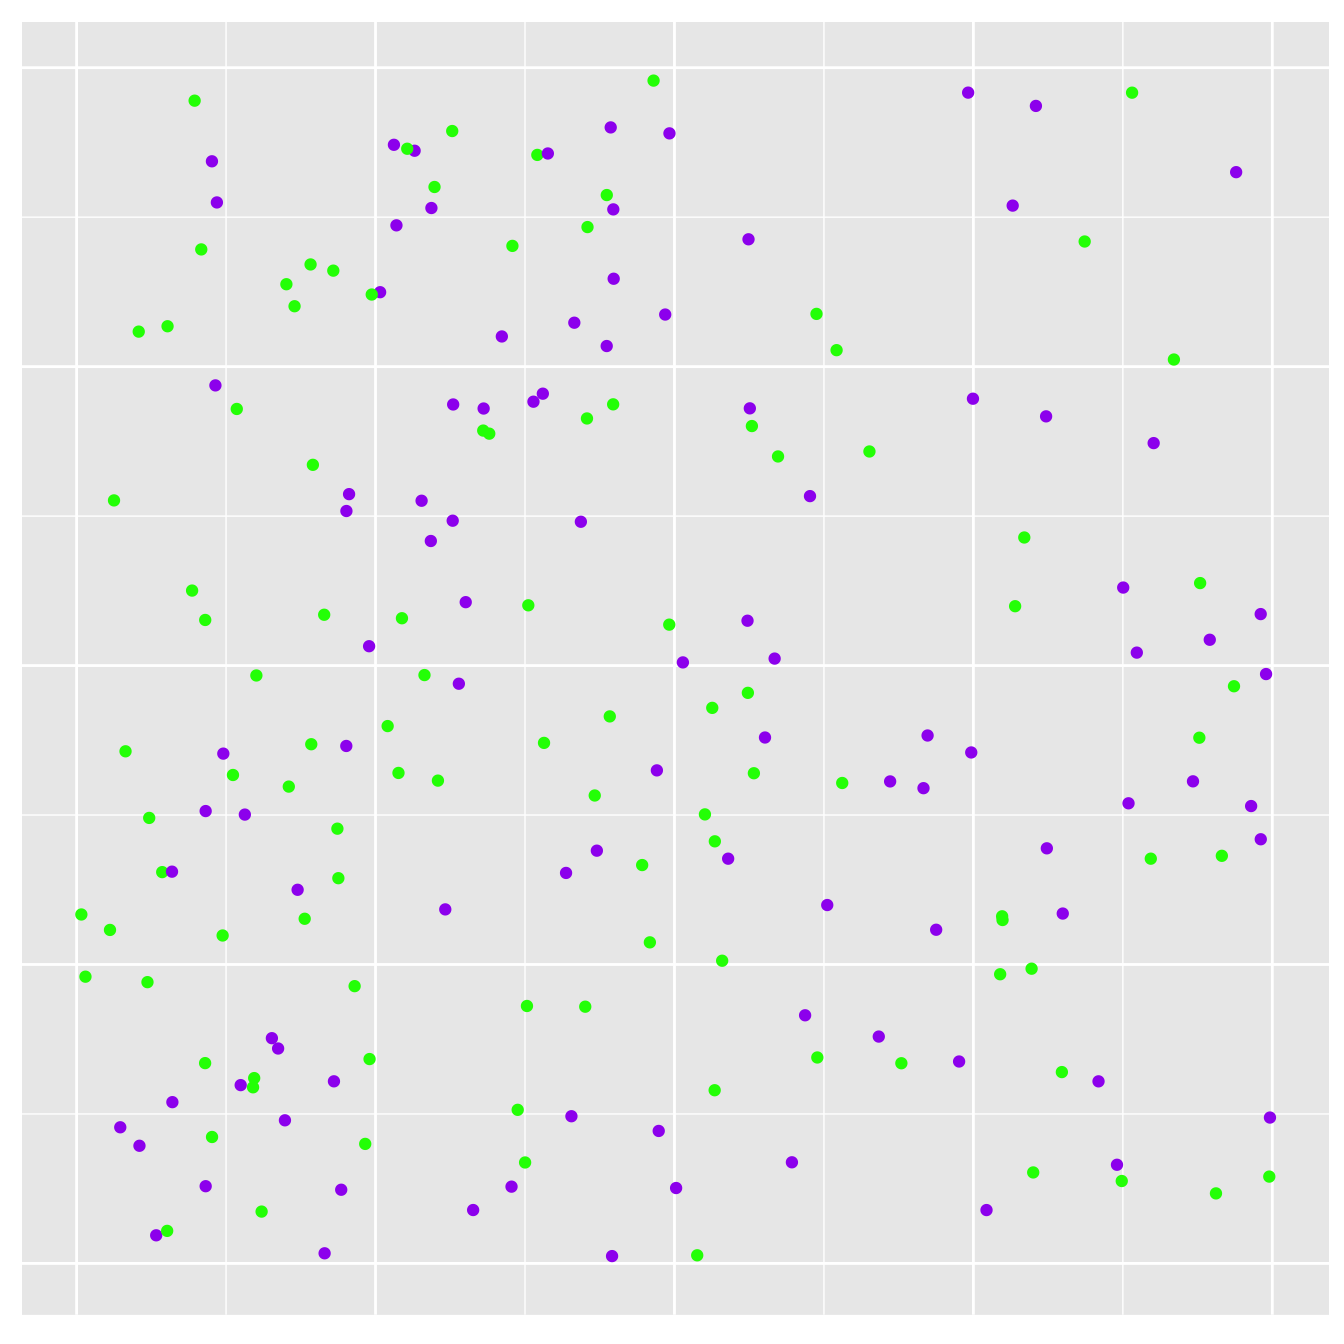
\includegraphics[width=0.5\linewidth]{stats-for-bio_files/figure-latex/plants-all-1} 

}

\caption{Stylised landscape showing a population of purple and green plants}\label{fig:plants-all}
\end{figure}

These idealised data were generated using a simulation in R. The details
of how we did this aren't important, but basically, we placed
`individuals' onto the landscape at random locations (every location is
equally likely), and then assigned them purple morph status with a
certain probability (we made them green otherwise). We'll come back to
the probability we actually used in the next chapter. Let's proceed as
though this were a real situation\ldots{}

\textbf{Step 1: Refine your questions, hypotheses and predictions}

Imagine we had previously been studying a neighbouring population that
exhibits the same polymorphism. We're fairly sure both populations were
once connected, but habitat loss over the last few hundred years has
significantly reduced gene flow between them. Our studies with the
neighbouring population have shown that\ldots{}

\begin{itemize}
\item
  The colour polymorphism is controlled by a single gene with two
  alleles: a recessive mutant allele (`P') confers the purple colour,
  and the dominant wild-type allele (`G') makes plants green. Population
  genetic studies have shown that the two alleles are present in a ratio
  of about 1:1.
\item
  There seems to be no observable fitness difference between the two
  morphs in the neighbouring population. What's more, about 25\% of
  plants are purple, i.e.~the alleles seem to be in
  \href{https://en.wikipedia.org/wiki/Hardy–Weinberg_principle}{Hardy-Weinberg
  equilibrium}. These two observations indicate that there is no
  selection operating on the polymorphism (it's `neutral').
\end{itemize}

Things are different in the new study population. The purple morph seems
to be about as common as the green morph. What's more, some preliminary
work indicates that purple plants seem to produce more seeds than green
plants. Our hypothesis is, therefore, that purple plants have a
selective advantage in the new study population. The corresponding
prediction is that the frequency of the purple morph will be greater
than 25\% in the new study population, as selection should be driving
the `P' allele to fixation.

(This isn't the strongest test of our hypothesis, by the way. Really, we
need to study allele and genotype frequencies, not just phenotypes.
Sadly, since Brexit happened, the government has pulled the research
funding for genetic research on plant polymorphism, so this is the best
we can do.)

\textbf{Step 2: Decide which population is important}

Our situation is made up, so questions about the statistical population
are not hugely relevant to be honest. In reality, we would consider
various factors, such as whether we can study the whole population or
need to restrict ourselves to a smaller scale (e.g.~to one
sub-population). Working at a large scale should produce a more general
result, but it could also present a significant logistical challenge.

\textbf{Step 3: Decide which variables to study}

This step is easy in this example. We could measure all kinds of
different attributes of our plants---biomass, height, seed production,
etc---but to study the polymorphism, we only need to collect information
about the colour of different individuals. This means we are going to be
working with a nominal (i.e.~categorical) variable, which takes two
values: `purple' or `green'.

\textbf{Step 4: Decide which population parameters are relevant}

The prediction we want to test is about the purple morph frequency (or
equivalently, the percentage, or proportion, of purple plants).
Therefore, the relevant population parameter is the frequency of purple
morphs in the wider population. We need to collect `data' so that we can
learn about this unknown quantity.

\textbf{Step 5: Gather a representative sample}

A representative sample here is one in which every individual on the
landscape has the same probability of being sampled (i.e.~a `random
sample'). Gathering a random sample of organisms from across a landscape
is surprisingly hard to do in reality, but it is at least easy to do in
a simulation. Let's seen what happens if we sample 20 plants at
random\ldots{}

\begin{figure}

{\centering 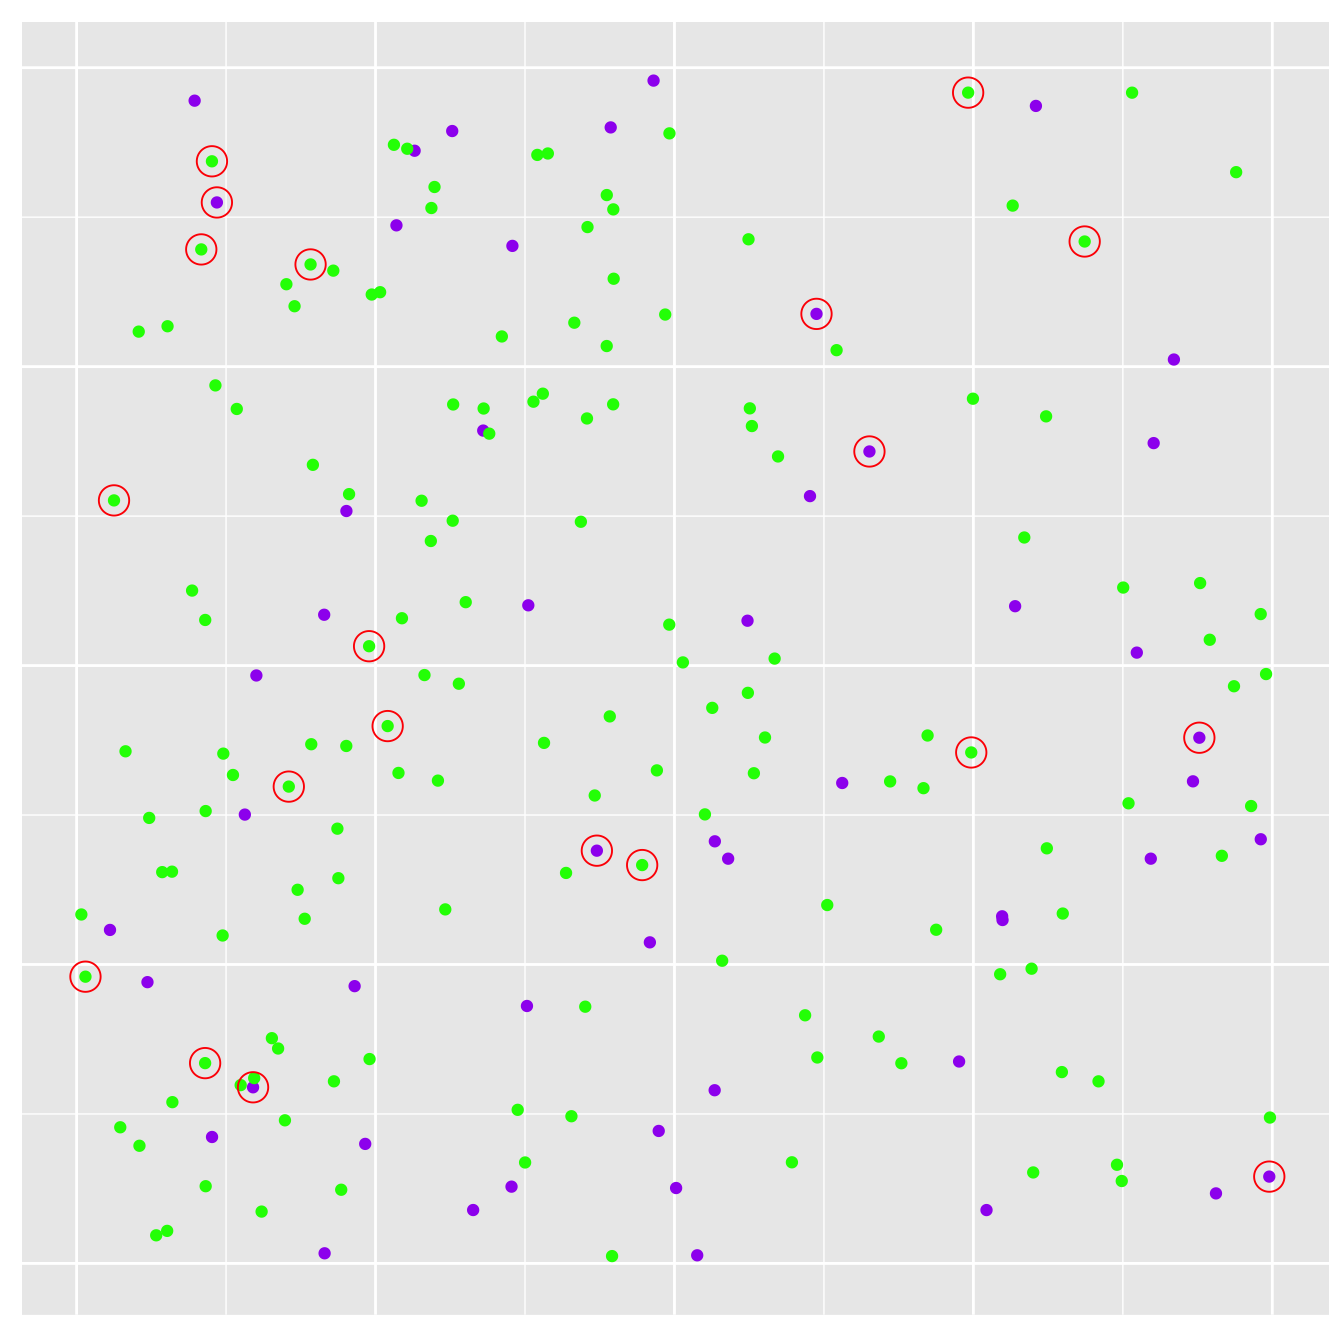
\includegraphics[width=0.5\linewidth]{stats-for-bio_files/figure-latex/plants-samp1-1} 

}

\caption{Sampling plants. Sampled plants are circled in red}\label{fig:plants-samp1}
\end{figure}

The new plot shows the original population of plants, only this time
we've circled the sampled individuals in red.

\textbf{Step 6: Estimate the population parameter}

Estimating a frequency from a sample is simple enough. We can express a
frequency in different ways. Let's use a percentage. We found 13 green
plants and 7 purple plants in our sample, which means our point estimate
of the purple morph frequency is 35\%. This is certainly greater than
25\%---the value of observed in the original population---but it isn't
that far off.

Maybe the purple plants aren't at a selective advantage after all? Or
maybe they are? We'll eventually see how to use a statistical test to
rigorously evaluate our prediction. First we need to learn a few more
concepts. Time to learn about something called sampling error\ldots{}

\chapter{Sampling error}\label{sampling-error}

In the previous chapter we introduced the idea that a point estimate of
a population parameter will be imperfect, in the sense that it won't
exactly reflect the true value of that parameter. This uncertainty is
always present, so it's not enough to have just estimated something. We
have to know about the uncertainty (i.e.~the precision) of the estimate.
We use the machinery of statistics to quantify this uncertainty.

Once we have pinned down the uncertainty we can start to provide
meaningful answers to our scientific questions. We will arrive at this
`getting to the answer step' in the next chapter. First we have to
develop the uncertainty idea a bit more. We need to learn about sampling
error, sampling distributions and standard errors.

\hypertarget{sampling-error-1}{\section{Sampling
error}\label{sampling-error-1}}

Let's carry on with the plant polymorphism example from the previous
chapter: the green-purple plant polymorphism. Skim back over the example
if you can't remember it, as you need to know what we're trying to do
for this chapter to be useful. So far, we had taken one sample of 20
plants from our hypothetical population and found that the frequency of
purple plants in that sample was 35\%. This is a point estimate of
purple plant frequency based on a random sample of 20 plants.

What happens if we repeat the same process, leading to a new, completely
independent sample? Here's a reminder of what the population looked
like, along with a new sample highlighted with red circles:

\begin{figure}

{\centering 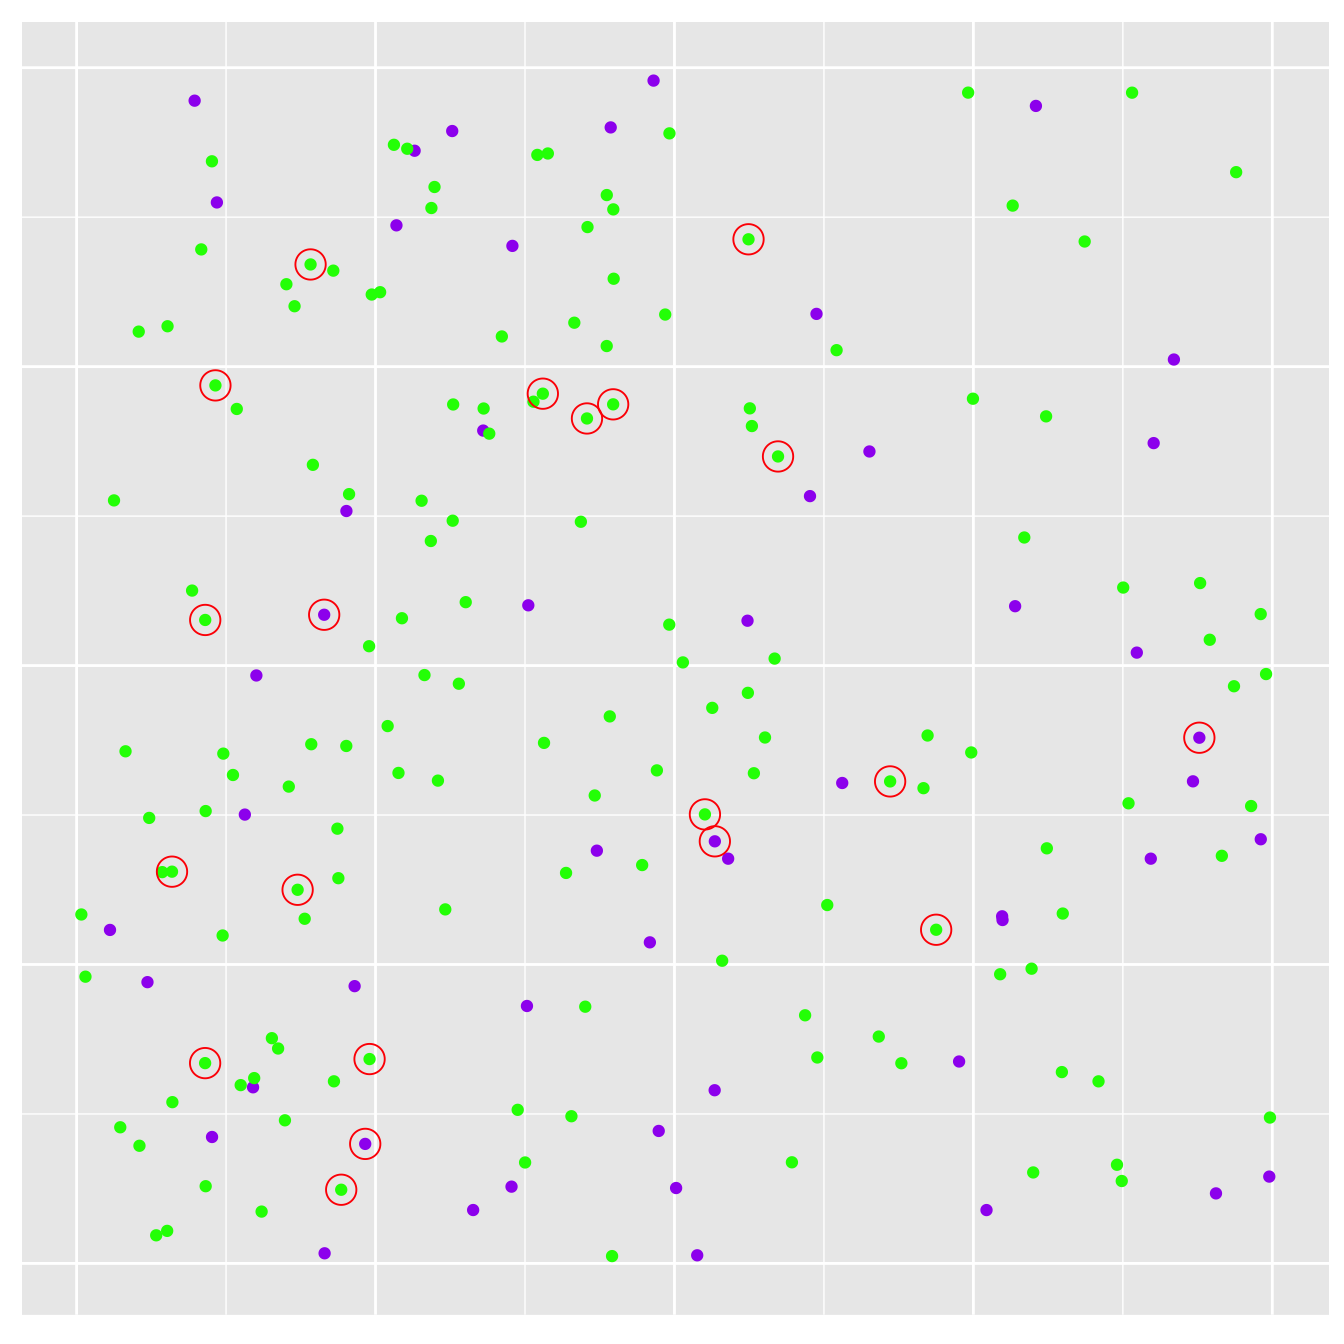
\includegraphics[width=0.5\linewidth]{stats-for-bio_files/figure-latex/plants-samp2-1} 

}

\caption{Plants sampled on the second occasion}\label{fig:plants-samp2}
\end{figure}

This time we ended up sampling 16 green plants and 4 purple plants, so
our second estimate of the purple morph frequency is 20\%. This is quite
different from the first estimate. Notice that it is actually lower than
that seen in the original study population. Our hypothesis that the
purple morph will be more prevalent in the new study population is
beginning to look a little shaky\ldots{}

Note that nothing about the study population changed between the first
and second sample. What's more, we used a completely reliable sampling
scheme to generate these samples (you'll have to trust us on that one).
There was nothing biased or `incorrect' about the way individuals were
sampled---every individual had the same chance of being selected. The
two different estimates of the purple morph frequency simply arise from
chance variation in selection. This variation, which arises whenever we
observe a sample instead of the whole population, has a special name. It
is called the \textbf{sampling error}.

(Another name for sampling error is `sampling variation'. Which one is
better? Neither really. We tend to use both terms---`sampling error' and
`sampling variation'---in this book because they are both widely used.)

Sampling error is the main reason why we have to use statistics. Any
estimate you derive from a sample is affected by it. Sampling error is
not really a property of any particular sample though. The form of
sampling error in any given problem is a consequence of the population
distribution of the variable(s) we're studying, and the sampling method
used to investigate this. That may seem a little cryptic now. Don't
worry, we will start to get a sense of what it really means in this
chapter.

\section{Sampling distributions}\label{sampling-distributions}

We can develop our simple simulation example a bit more to explore the
consequences of sampling error. However, rather than taking one sample
at a time, we'll use R to simulate thousands of independent samples. The
number of plants sampled (`n') will always be 20. Here's the important
bit: every sample is drawn from the same population, i.e.~the population
parameter (purple morph frequency) will never change across samples.
This means any variation we observe will be due to nothing more than
sampling error.

Here is a summary of one such repeated simulation exercise:

\begin{figure}

{\centering 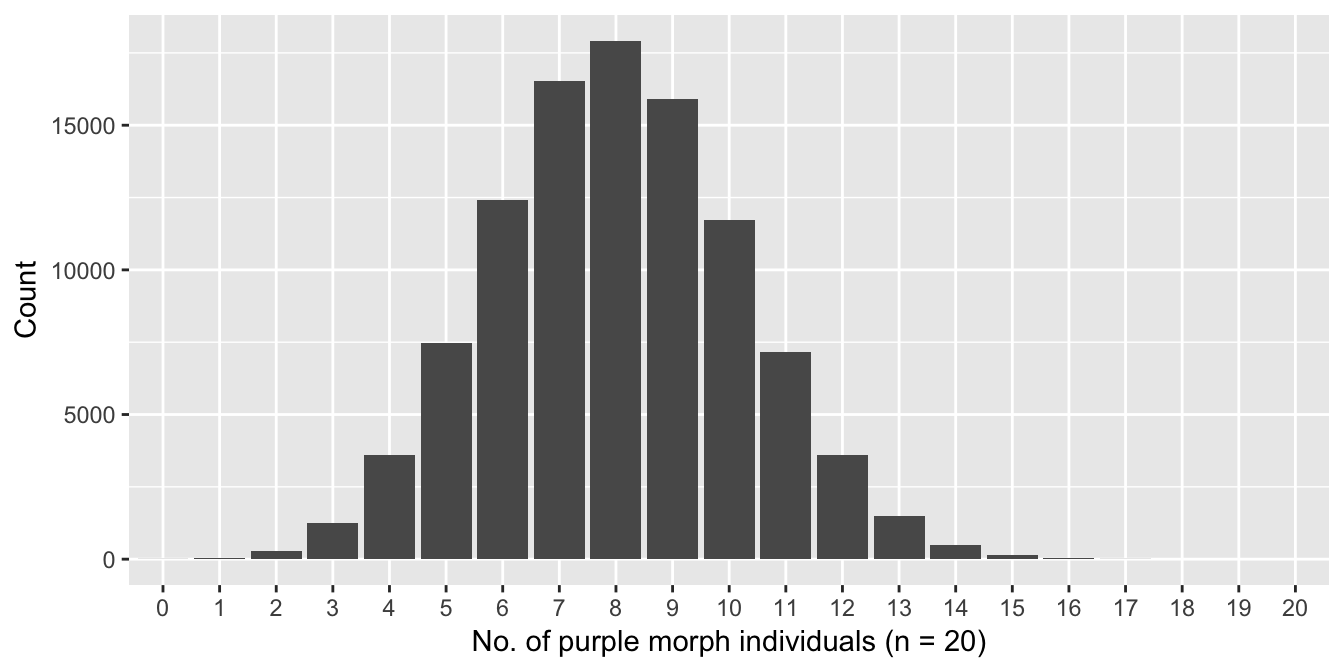
\includegraphics[width=1\linewidth]{stats-for-bio_files/figure-latex/samp-dist-1-1} 

}

\caption{Distribution of number of purple morphs sampled (n = 20)}\label{fig:samp-dist-1}
\end{figure}

This bar plot summarises the result from 100000 samples. In each sample,
we took 20 individuals from our hypothetical population and calculated
the number of purple morphs found. The bar plot shows the number of
times we found 0, 1, 2, 3, \ldots{} purple individuals, all the way up
to the maximum possible (20). We could have converted these numbers to
frequencies, but instead we're just summarising the raw distribution of
purple morph counts that we found. This distribution has a special name.
It is called a \textbf{sampling distribution}.

The sampling distribution is just the distribution we expect a
particular estimate (or more generally, a `statistic') to follow. In
order to to work this out, we have to postulate values for the
population parameters, and we have to know how the population was
sampled. Rather than use mathematical reasoning, we used brute-force
simulation to approximate the sampling distribution of purple morph
counts that arises when we sample 20 individuals from our hypothetical
population.

What does the sampling distribution show? It shows us the range of
outcomes we can expect when we repeat the same sampling process over and
over again. The most common outcome is 8 purple morphs, which would
yield an estimate of 8/20 = 40\% for the purple morph frequency. This is
the frequency that was actually used to simulate the data (we didn't
tell you that before). The population parameter we're trying to learn
about turns out to be the most common point estimate we should expect to
see under repeated sampling.

(So now we know the answer to our question. The purple morph frequency
is 40\%. Of course we cheated though, because we used information from
1000s of samples. In the real world we only have one, limited sample.)

The sampling distribution is the key to `doing statistics'. Look at the
spread (dispersion) of the sampling distribution above. The range of
outcomes is roughly 2 to 15, which corresponds to estimated frequencies
of the purple morph in the range of 10-75\%, because we sampled 20
individuals on each occasion. This tells us that when we sample only 20
individuals, the sampling error is expected to be quite large.

Note that the sampling distribution we summarised above is only relevant
for the case where 20 individuals are sampled, and the frequency of
purple plants in the population is 40\%. If we change either of those
two things we would end up with a different sampling distribution.
That's what we meant when we said, ``The form of sampling error in any
given problem is a consequence of the population distribution of the
variable(s) we're studying, and the sampling method used to investigate
this.''

Once we know how to calculate the sampling distribution for a particular
problem, we can start to make statements about sampling error (to
quantify uncertainty), and we can begin to make meaningful comparisons
to address scientific questions. We don't have to work any of this out
for ourselves --- statisticians have done the hard work for us.

\section{The effect of sample size}\label{the-effect-of-sample-size}

One of the most important aspect of a sampling scheme is the
\textbf{sample size} (denoted `n'). This is just the number of
observations (individuals, objects, items, etc) in a sample. What
happens when we change the sample size?

We'll carry on with the example to see how sample size influences the
sampling distribution, and to understand why it matters. Let's repeat
the multiple sampling exercise, but this time do it with two different
sample sizes. First we'll use a sample size of 40 individuals, and then
we'll take a sample of 80 individuals each time. As before, we'll take a
total 100000 samples each time:

\begin{figure}

{\centering 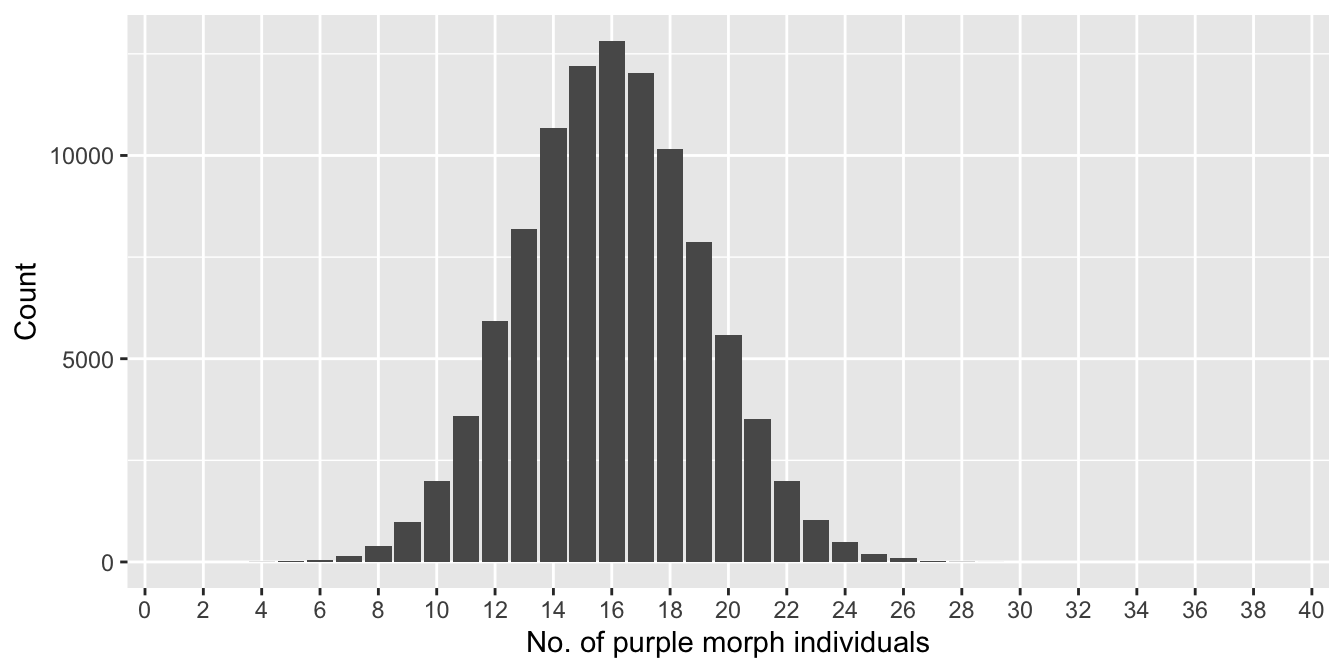
\includegraphics[width=1\linewidth]{stats-for-bio_files/figure-latex/samp-dist-2-1} 

}

\caption{Distribution of number of purple morphs sampled (n = 40)}\label{fig:samp-dist-2}
\end{figure}

\begin{figure}

{\centering 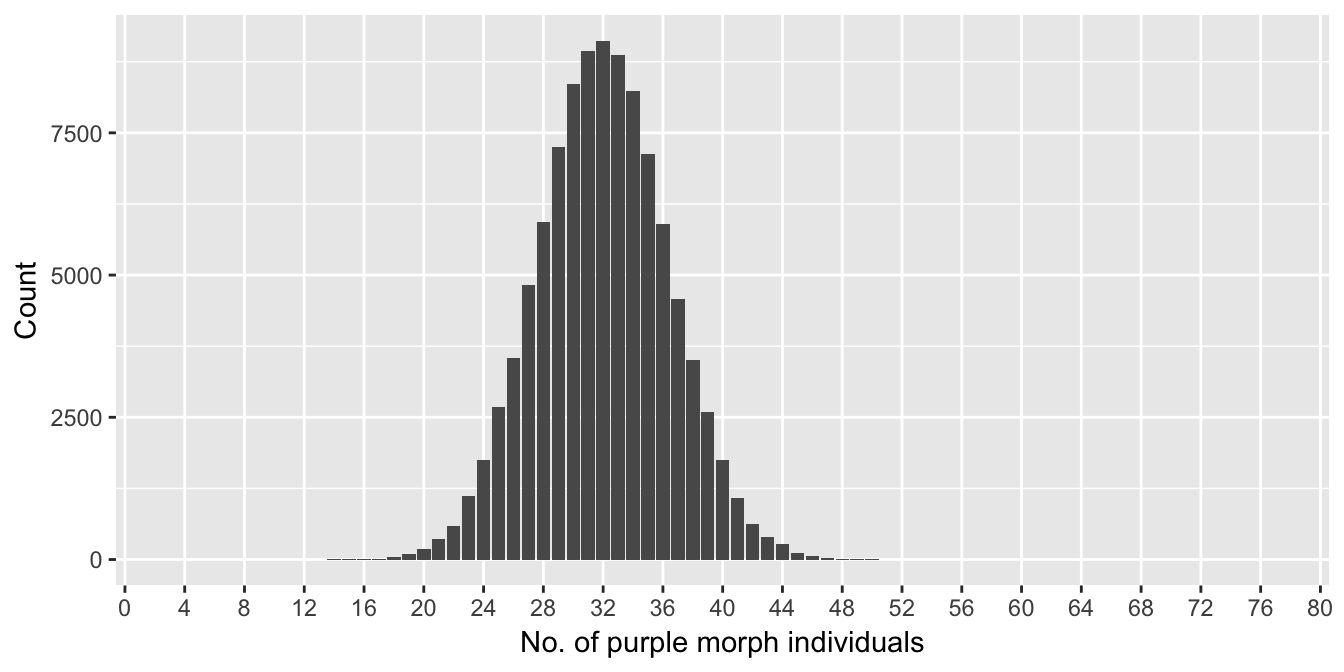
\includegraphics[width=1\linewidth]{stats-for-bio_files/figure-latex/samp-dist-3-1} 

}

\caption{Distribution of number of purple morphs sampled (n = 80)}\label{fig:samp-dist-3}
\end{figure}

What do these plots tell us about the effect of changing sample size?
Notice that we plotted each of them over the full range of possible
outcomes (the x axis runs from 0-40 and 0-80, respectively, in the first
and second plot). This is so we can meaningfully compare the spread of
each sampling distribution relative to the range of possible outcomes.

The range of outcomes in the first plot (n = 40) is roughly 6 to 26,
which corresponds to estimated frequencies of the purple morph in the
range of 15-65\%. The range of outcomes in the second plot (n = 80) is
roughly 16 to 48, which corresponds to estimated frequencies in the
range of 20-60\%. The implications of this not so rigorous assessment
are probably obvious. When we increase the sample size we can expect to
encounter less sampling error. This makes intuitive sense: the
composition of a large sample should more closely approximate that of
the true population than a small sample.

How much data do we need to collect to accurately estimate a frequency?
Here is the approximate sampling distribution of the purple morph
frequency estimate when we sample 500 individuals:

\begin{figure}

{\centering 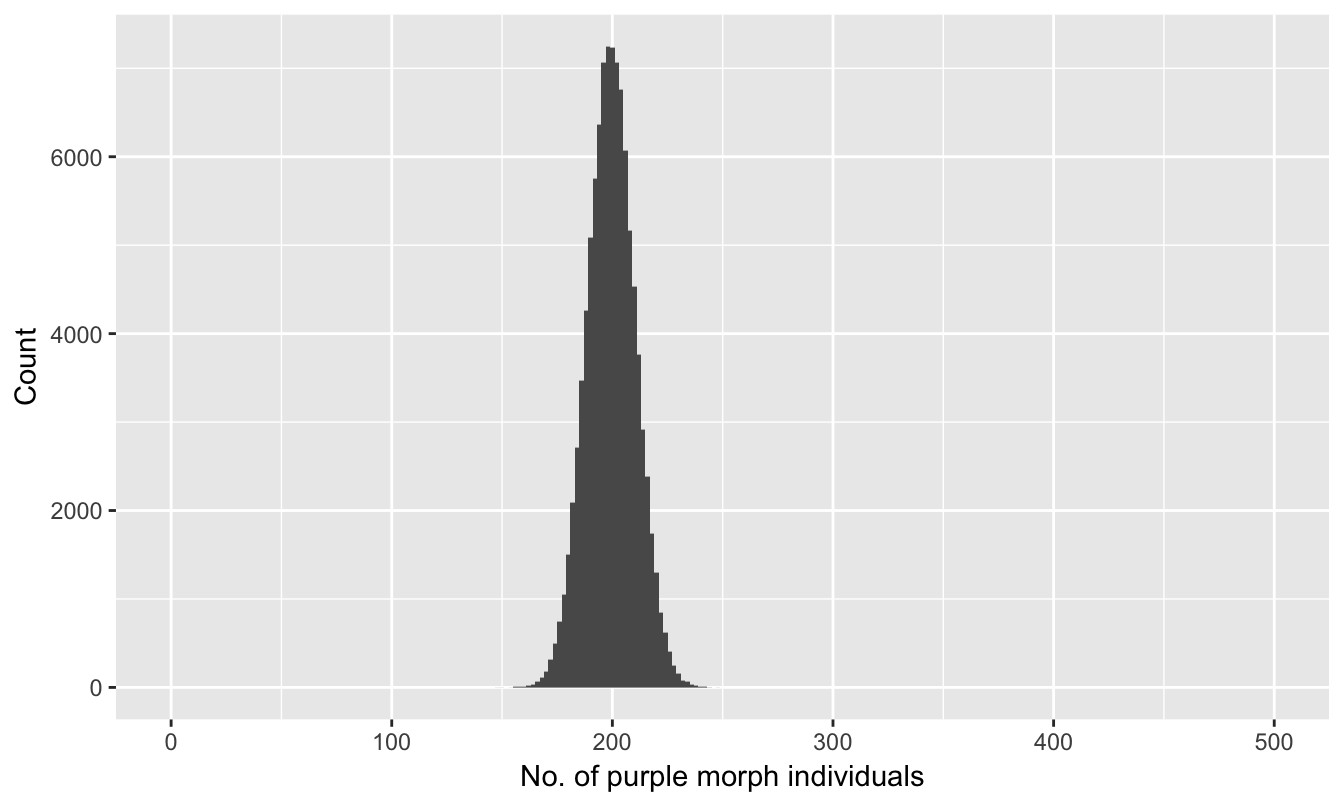
\includegraphics[width=1\linewidth]{stats-for-bio_files/figure-latex/samp-dist-big-1} 

}

\caption{Distribution of number of purple morphs sampled (n = 500)}\label{fig:samp-dist-big}
\end{figure}

Now the range of outcomes is about 160 to 240, corresponding to purple
morph frequencies in the 32-48\% range. This is a big improvement over
the smaller samples that we just considered, but even with 500
individuals in a sample, we should still expect quite a lot of
uncertainty in our estimate. The take home message is that you need a
lot of data to reduce sampling error.

\section{The standard error}\label{the-standard-error}

We've been fairly relaxed about how we quantified the spread of a
sampling distribution up until this point. We just estimated the
approximate range of purple morph counts ``by eye''. This is fine for
investigating general patterns, but to make rigorous comparisons, we
really need a quantitative measure of this variability. This is called
the \textbf{standard error}.

The standard error is actually quite a simple idea, though its
definition often causes confusion. Here is that definition: a standard
error is the standard deviation of the sampling distribution of an
estimate, like a mean or a frequency. Don't worry if that makes
absolutely no sense. The key point is that it is a standard deviation,
so it a measure of the spread, or dispersion, of a distribution. The
distribution in the case of a standard error is the sampling
distribution of some kind of estimate.

(It is common to use a shorthand abbreviations such ``SE'', ``S.E.'',
``se'' or ``s.e.'' in place of `standard error' when referring to the
standard error in text.)

We can use a simulation in R to calculate the expected standard error of
an estimate of purple morph frequency. In order to do this we have to
specify the value of the population frequency, and we have to decide
what sample size we want to evaluate.

Let's find the expected standard error when the purple morph frequency
is 40\% and the sample size is 80. First we set up the simulation by
assigning values to different variables to control what the simulation
does:

\begin{Shaded}
\begin{Highlighting}[]
\NormalTok{purple_prob <-}\StringTok{ }\FloatTok{0.4}
\NormalTok{sample_size <-}\StringTok{ }\DecValTok{80}
\NormalTok{n_samples <-}\StringTok{ }\DecValTok{100000}
\end{Highlighting}
\end{Shaded}

The value of \texttt{purple\_prob} is the probability a plant will be
purple (0.4 --- R doesn't like percentages), the value of
\texttt{sample\_size} is the sample size for each sample, and the value
of \texttt{n\_samples} is the number of independent samples we'll take.
That's simple enough.

\begin{Shaded}
\begin{Highlighting}[]
\NormalTok{raw_samples <-}\StringTok{ }\KeywordTok{rbinom}\NormalTok{(}\DataTypeTok{n =} \NormalTok{n_samples, }\DataTypeTok{size =} \NormalTok{sample_size, }\DataTypeTok{prob =} \NormalTok{purple_prob)}
\NormalTok{percent_samples <-}\StringTok{ }\DecValTok{100} \NormalTok{*}\StringTok{ }\NormalTok{raw_samples /}\StringTok{ }\NormalTok{sample_size}
\end{Highlighting}
\end{Shaded}

You don't have to understand how this works, but if you did A-level
statistics you might be able to guess what the \texttt{rbinom} function
is doing. Honestly though, the R code isn't important here. We're just
showing it to you to demonstrate that seemingly complex simulations are
often easy to do in R. It is more or less the same code we used to
generate those plots above (the only difference is that this time we
converted the numbers into proportions).

The result is what matters. We simulated the percentage of purple morph
individuals found in 100000 samples of 20 individuals, assuming the
purple morph frequency is always 40\%. The results are stored the result
in a vector called \texttt{percent\_samples}. Here are the first 50
values of that vector:

\begin{Shaded}
\begin{Highlighting}[]
\KeywordTok{head}\NormalTok{(percent_samples, }\DecValTok{50}\NormalTok{)}
\end{Highlighting}
\end{Shaded}

\begin{verbatim}
##  [1] 42.50 37.50 36.25 30.00 35.00 35.00 51.25 35.00 41.25 36.25 32.50
## [12] 37.50 32.50 38.75 37.50 36.25 33.75 35.00 42.50 41.25 46.25 35.00
## [23] 42.50 45.00 43.75 40.00 41.25 52.50 43.75 38.75 38.75 47.50 42.50
## [34] 40.00 43.75 42.50 36.25 42.50 43.75 43.75 35.00 42.50 35.00 37.50
## [45] 41.25 40.00 45.00 40.00 41.25 38.75
\end{verbatim}

These numbers are all part of the sampling distribution of morph
frequency estimates. So\ldots{} how to calculate the standard error?
This is the standard deviation of these numbers, so we just use the
\texttt{sd} function:

\begin{Shaded}
\begin{Highlighting}[]
\KeywordTok{sd}\NormalTok{(percent_samples)}
\end{Highlighting}
\end{Shaded}

\begin{verbatim}
## [1] 5.494687
\end{verbatim}

Why is this useful? The standard error gives us a standard means to
compare the variability we expect to see, or the variability we actually
see, in different sampling distributions. As long as the sampling
distribution is `well-behaved', then, roughly speaking, most estimates
(\textasciitilde{}95\%) can be expected to lie in a range of about four
standard errors. If you're not convinced, look at the second bar plot we
produced above (where the sample size = 80, and the purple morph
frequency = 40\%). What is the approximate range of simulated values?
How close is this to \(4 \times 5.5\)? Pretty close we think\ldots{}

So in summary, the standard error gives us a way to quantify how much
variability we expect to see in a sampling distribution. We said in the
previous chapter (\protect\hyperlink{learning-from-data}{Learning from
data}) that a point estimate is useless without some kind of associated
measure of uncertainty. A standard error is one such measure.

\section{What is the point of all
this!?}\label{what-is-the-point-of-all-this}

By this point you might (quite reasonably) be wondering why we have
spent so much time looking at properties of repeated samples from a
population. After all, when we collect data in the real world we'll only
have a single sample to work with. We can't just keep collecting more
and more data. We also won't know anything about the population
parameter of interest. This lack of knowledge is the reason for
collecting the data in the first place!

The short answer to this question is that before we can start to use
frequentist statistics---remember, that's our ultimate goal---we need to
have a sense of\ldots{}

\begin{itemize}
\item
  how point estimates behave under repeated sampling (i.e.~sampling
  distributions),
\item
  and how `sampling error' and `standard error' relate to sampling
  distributions.
\end{itemize}

Once we understand these links, we're able to start exploring the
techniques that underlie frequentist statistics. That's what we'll do in
the next block of work\ldots{}

\part{Statistical Concepts
(II)}\label{part-statistical-concepts-ii}
\addcontentsline{toc}{chapter}{(PART) Statistical Concepts (II)}

\chapter{\texorpdfstring{Statistical significance and
\emph{p}-values}{Statistical significance and p-values}}\label{statistical-significance-and-p-values}

We have already pointed out that we use frequentist statistics in this
book. While it isn't possible to give a precise description of how
frequentist statistics works in an introductory book, we can at least
provide a rough indication. Frequentist statistics works by asking
\emph{what would have happened} if we were to repeat an experiment or
data collection exercise many times, \emph{assuming that the relevant
population parameters remain the same} each time. That was the basic
idea we employed to generate those sampling distributions in the last
chapter.

The choice of population parameter(s) to work with depend on what kind
of question we are asking. This obviously varies from one situation to
another. The thing that is common to every frequentist technique is that
we ultimately have to work out how a sampling distribution of some kind
should look. If we can do that, then we can ask, for a given scenario,
how likely or unlikely a particular result is. This naturally leads onto
two of the most important ideas in this book: statistical significance
and \emph{p}-values. The goal of this chapter is to introduce these
ideas.

\section{Estimating a sampling distribution}\label{bootstrap}

Let's carry on with the plant polymorphism example (yes, again). Our
ultimate goal is to evaluate whether the purple morph frequency is
greater than 25\% in the new study population. The suggestion in the
preamble of this chapter is that, to get to this point, we need to work
out what the sampling distribution of the purple morph frequency
estimate looks like. At first glance this seems like an impossible task.
We can't use simulations, because we don't know the true frequency of
purple morphs in the population. All we have is the one sample.

The solution to this problem is surprisingly simple (or at least the
basic idea is simple): since we don't know much about the population, we
use the sample to approximate some aspect(s) of it, and then work out
what the sampling distribution of our estimate should look like using
this approximation.

Let's unpack this idea a bit more, and then try it out for real.

\subsection{Overview of bootstrapping}\label{bootstrap-overview}

There are many different ways to approximate a population from a sample.
One of the simplest methods---for easy problems at least---is to
\emph{pretend the sample is the true population}. Then, all we have to
do to get at a sampling distribution is draw new samples from this
pretend population. That may sound a lot like cheating, but it turns out
that this is a perfectly valid way to construct useful sampling
distributions for many kinds of problems.

Here is how it works for our example, using a physical analogy. Imagine
that we only have one sample, and have written down the colour of each
sampled plant on a different piece of paper, and then placed all of
these bits of paper into in a hat. We then do the following:

\begin{enumerate}
\def\labelenumi{\arabic{enumi}.}
\tightlist
\item
  Pick a piece of paper at random, record its value (purple or green),
  put the paper back into the hat, and shake the hat about to mix up the
  bits of paper.
\end{enumerate}

(The shaking here is meant to ensure that each piece of paper has an
equal chance of being picked, i.e.~we're taking a random sample. This
might not work in reality, but let's assume it does.)

\begin{enumerate}
\def\labelenumi{\arabic{enumi}.}
\setcounter{enumi}{1}
\item
  Pick another piece of paper (you might get the same one), record its
  value, and then put that back into the hat, remembering to shake
  everything up.
\item
  Repeat this process until we have a recorded new sample of colours
  which is the same size as your real sample. Now we have a `new
  sample'.
\end{enumerate}

(This process is called `sampling with replacement'. Each artificial
sample is called a `bootstrapped sample'.)

\begin{enumerate}
\def\labelenumi{\arabic{enumi}.}
\setcounter{enumi}{3}
\item
  For each bootstrapped sample, calculate whatever quantity is of
  interest. In our example, this is the proportion of purple plants
  sampled.
\item
  Repeat steps 1-4 until we have generated a large number of
  bootstrapped samples. About 10000 is often sufficient for many
  problems.
\end{enumerate}

Although it may seem like cheating (it's not!), this process really does
produce an approximation of the sampling distribution of the quantity
we're interest in. It is called \textbf{bootstrapping} (or `the
bootstrap'). The bootstrap was invented by a very smart statistician
called \href{https://en.wikipedia.org/wiki/Bradley_Efron}{Bradley
Efron}. We're introducing it here because it allows you to see how
frequentist methodology works without having to do any nasty
mathematics. We're not expecting you to learn it, so don't worry too
much if you find it tricky to understand. It is an odd concept.

\subsection{Doing it for real}\label{doing-it-for-real}

Let's assume we've sampled 250 individuals from our new plant
population. We're going to use this hypothetical sample to implement the
bootstrap in R.

\begin{do-something}
The best way to understand what follows is to actually work through the
example. You're strongly encouraged to do this\ldots{}
\end{do-something}

A data set representing this situation is stored in a Comma Separated
Value (CSV) text file called `MORPH\_DATA.CSV'. Download the file from
MOLE and place it in your working directory (you should set this at the
beginning of the R session). Next, run through the following steps:

\begin{itemize}
\item
  Read the data into an R data frame using \texttt{read.csv}, assigning
  the data frame the name \texttt{morph.data}.
\item
  Use a function like \texttt{glimpse} (from \textbf{dplyr}) or
  \texttt{str} (from base R) to inspect the structure of
  \texttt{morph.data}. How many variables are in the data set? What are
  their names? What kind of variables are they?
\item
  Use the \texttt{View} function to inspect the data. Is this what you
  expected? Are the values of the different variables as you would
  expect them to be?
\end{itemize}

The point of all this is to `sanity check' the data, i.e.~to make sure
we understand the data and that there are no obvious problems with it.
\textbf{We should always check our data after we've read it in}. There
is really no point messing about with the likes of \textbf{dplyr} and
\textbf{ggplot2}, or carrying out a statistical analysis, until we have
done this. If we don't understand how our data is organised, and what
variables we are working with, there is a very real risk that we will
make a lot of avoidable mistakes.

What you should have found is that \texttt{morph.data} contains 250 rows
and two columns/variables: \texttt{Colour} and \texttt{Weight}.
\texttt{Colour} is a categorical variable (a `factor', in R-land) and
\texttt{Weight} is a numeric variable. The \texttt{Colour} variable
obviously contains the colour of each plant in the sample. What about
\texttt{Weight}? We don't need this now, but we'll use it in the next
chapter.

Now that we understand the data, we're ready to implement bootstrapping
(using R of course, no hats or paper required). We're going to introduce
a few new R tricks here. We'll explain them as we go, but if you're not
a huge R fan, there's really no need to remember them. Focus on the
logic of what we're doing.

We want to construct a sampling distribution for the frequency of purple
morphs, so the variable that matters here is \texttt{Colour}. Rather
than work with this inside the data frame, we're going to pull it out
using the \texttt{\$} operator, assign it a name
(\texttt{plant\_morphs}), and then take a look at the first 20 values:

\begin{Shaded}
\begin{Highlighting}[]
\NormalTok{plant_morphs <-}\StringTok{ }\NormalTok{morph.data$Colour}
\KeywordTok{levels}\NormalTok{(plant_morphs)}
\end{Highlighting}
\end{Shaded}

\begin{verbatim}
## [1] "Green"  "Purple"
\end{verbatim}

\begin{Shaded}
\begin{Highlighting}[]
\KeywordTok{head}\NormalTok{(plant_morphs, }\DecValTok{100}\NormalTok{) }\CommentTok{# just show the first 100 values}
\end{Highlighting}
\end{Shaded}

\begin{verbatim}
##   [1] Green  Green  Green  Purple Green  Green  Green  Green  Green  Green 
##  [11] Green  Green  Green  Purple Green  Green  Purple Purple Green  Green 
##  [21] Green  Green  Green  Purple Green  Green  Green  Green  Purple Purple
##  [31] Green  Green  Green  Purple Purple Green  Green  Green  Green  Purple
##  [41] Green  Purple Green  Green  Purple Purple Green  Green  Green  Green 
##  [51] Green  Green  Purple Purple Purple Green  Green  Green  Purple Green 
##  [61] Purple Green  Purple Green  Purple Purple Green  Green  Purple Green 
##  [71] Green  Purple Purple Green  Purple Green  Green  Green  Green  Purple
##  [81] Purple Green  Purple Green  Green  Green  Purple Purple Green  Purple
##  [91] Green  Green  Green  Green  Green  Green  Purple Green  Green  Green 
## Levels: Green Purple
\end{verbatim}

Hopefully you followed that---\texttt{plant\_morphs} is just a simple
vector (a factor, with 2 categories) containing the colour information.

Let's calculate and store the sample size (\texttt{samp\_size}), and the
point estimate of purple morph frequency (\texttt{mean\_point\_est})
from this sample:

\begin{Shaded}
\begin{Highlighting}[]
\NormalTok{samp_size <-}\StringTok{ }\KeywordTok{length}\NormalTok{(plant_morphs)}
\NormalTok{samp_size}
\end{Highlighting}
\end{Shaded}

\begin{verbatim}
## [1] 250
\end{verbatim}

\begin{Shaded}
\begin{Highlighting}[]
\NormalTok{mean_point_est <-}\StringTok{ }\DecValTok{100} \NormalTok{*}\StringTok{ }\KeywordTok{sum}\NormalTok{(plant_morphs ==}\StringTok{ "Purple"}\NormalTok{) /}\StringTok{ }\NormalTok{samp_size}
\NormalTok{mean_point_est}
\end{Highlighting}
\end{Shaded}

\begin{verbatim}
## [1] 30.8
\end{verbatim}

So\ldots{} 30.8\% of plants were purple among our sample of 250 plants.

We are now ready to start bootstrapping. We'll construct 10000 bootstrap
samples, and for convenience, we'll store this number in
\texttt{n\_samp}:

\begin{Shaded}
\begin{Highlighting}[]
\NormalTok{n_samp <-}\StringTok{ }\DecValTok{10000}
\end{Highlighting}
\end{Shaded}

We need to resample the \texttt{plant\_morphs} vector. The
\texttt{sample} function will do this for us (\texttt{replace\ =\ TRUE}
makes it sample with replacement):

\begin{Shaded}
\begin{Highlighting}[]
\NormalTok{samp <-}\StringTok{ }\KeywordTok{sample}\NormalTok{(plant_morphs, }\DataTypeTok{replace =} \OtherTok{TRUE}\NormalTok{)}
\KeywordTok{head}\NormalTok{(samp, }\DecValTok{100}\NormalTok{) }\CommentTok{# just show the first 100 values}
\end{Highlighting}
\end{Shaded}

\begin{verbatim}
##   [1] Purple Green  Green  Green  Purple Green  Green  Green  Purple Purple
##  [11] Green  Purple Green  Green  Green  Green  Purple Green  Green  Green 
##  [21] Green  Green  Green  Purple Green  Purple Green  Green  Green  Green 
##  [31] Green  Purple Purple Purple Green  Green  Green  Green  Green  Green 
##  [41] Green  Green  Purple Green  Green  Green  Purple Green  Green  Green 
##  [51] Green  Green  Green  Green  Green  Green  Purple Green  Green  Purple
##  [61] Purple Green  Green  Green  Green  Purple Purple Green  Green  Purple
##  [71] Green  Green  Green  Green  Purple Green  Green  Purple Green  Purple
##  [81] Green  Purple Green  Green  Green  Green  Green  Green  Green  Green 
##  [91] Green  Purple Green  Green  Green  Green  Green  Green  Purple Green 
## Levels: Green Purple
\end{verbatim}

Compare this one bootstrapped sample to the real one. It's a random
sample of the values in the first sample, as expected. We only need one
number from this sample, which is the frequency of purple morphs:

\begin{Shaded}
\begin{Highlighting}[]
\NormalTok{first_bs_freq <-}\StringTok{ }\DecValTok{100} \NormalTok{*}\StringTok{ }\KeywordTok{sum}\NormalTok{(samp ==}\StringTok{ "Purple"}\NormalTok{) /}\StringTok{ }\NormalTok{samp_size}
\KeywordTok{head}\NormalTok{(first_bs_freq, }\DecValTok{100}\NormalTok{) }\CommentTok{# just show the first 100 values}
\end{Highlighting}
\end{Shaded}

\begin{verbatim}
## [1] 27.2
\end{verbatim}

That's one bootstrapped value of purple morph frequency. Simple! We need
\(10^{4}\) values though, and we really don't want to have to keep doing
this over an over `by hand' (making \texttt{second\_bs\_freq},
\texttt{third\_bs\_freq}, and so on). That would be very dull\ldots{}

Fortunately, computers are very good at carrying out repetitive tasks
like this. Here is some R code that repeats what we just did
\texttt{n\_samp} times and stores the bootstrapped sample in a vector
called \texttt{boot\_out}:

\begin{Shaded}
\begin{Highlighting}[]
\NormalTok{boot_out <-}\StringTok{ }\KeywordTok{replicate}\NormalTok{(n_samp, \{}
  \NormalTok{samp <-}\StringTok{ }\KeywordTok{sample}\NormalTok{(plant_morphs, }\DataTypeTok{replace =} \OtherTok{TRUE}\NormalTok{)}
  \DecValTok{100} \NormalTok{*}\StringTok{ }\KeywordTok{sum}\NormalTok{(samp ==}\StringTok{ "Purple"}\NormalTok{) /}\StringTok{ }\NormalTok{samp_size}
\NormalTok{\})}
\end{Highlighting}
\end{Shaded}

The \texttt{replicate} function does exactly what you might think it
does. It replicates an R expression many times (\texttt{n\_samp} in this
case) and returns the set of results. Remember, you don't have to
understand this R code, but do ask a TA if you want to know more about
it.

The end result of the above is that \texttt{boot\_out} now contains a
bootstrapped sample of frequency estimates. Let's take a quick look at
the first 25 values, rounding each of them to 2 decimal places (we'll
used the pipe \texttt{\%\textgreater{}\%} to remind you it exists; just
keep in mind this won't work unless you have loaded the \textbf{dplyr}
package):

\begin{Shaded}
\begin{Highlighting}[]
\KeywordTok{head}\NormalTok{(boot_out, }\DecValTok{25}\NormalTok{) %>%}\StringTok{ }\KeywordTok{round}\NormalTok{(}\DecValTok{1}\NormalTok{)}
\end{Highlighting}
\end{Shaded}

\begin{verbatim}
##  [1] 26.0 28.0 32.0 26.8 32.8 35.6 31.2 32.4 33.6 30.0 27.6 29.6 30.8 34.0
## [15] 32.4 38.8 31.6 24.4 31.6 28.4 30.0 32.8 32.4 33.6 32.0
\end{verbatim}

These numbers represent different values of the purple morph frequency
that we might expect to generate if we repeated the data collection
exercise, assuming the observed purple morph frequency really is equal
to that of the actual sample. This is a bootstrapped sampling
distribution.

We can use this bootstrapped sampling distribution in a number of useful
ways. Let's plot it first get a sense of what it looks like. A histogram
is a good choice here because we have a reasonably large number of
cases:

\begin{figure}

{\centering 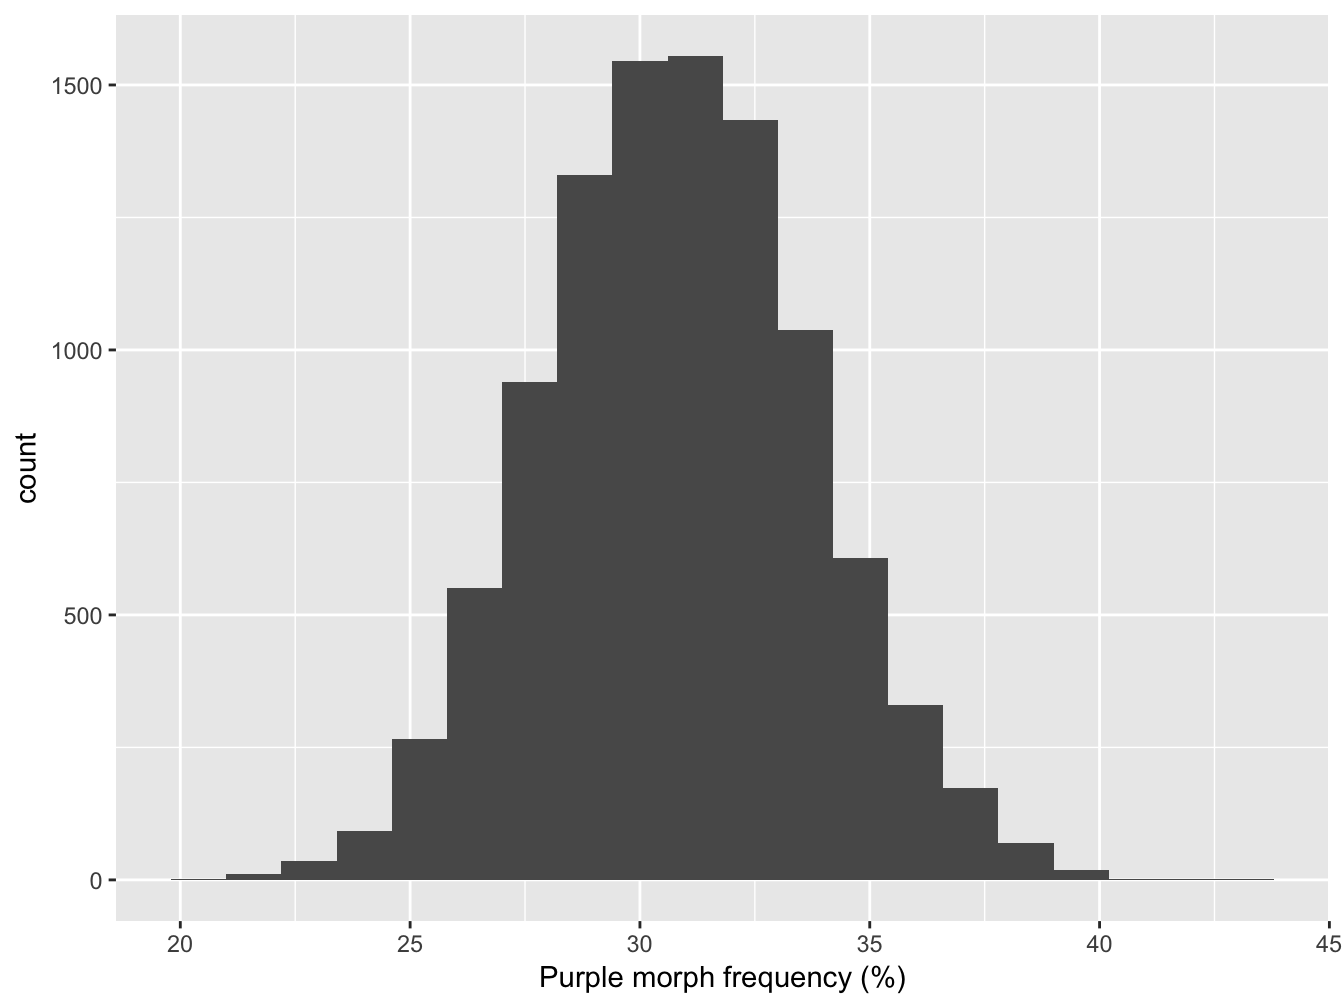
\includegraphics[width=0.75\linewidth]{stats-for-bio_files/figure-latex/boot-samp-dist-1} 

}

\caption{Bootstrapped sampling distribution of purple morph frequency}\label{fig:boot-samp-dist}
\end{figure}

The mean of the sampling distribution looks to be round about 31\%,
which is fairly close to the sample mean. We can of course calculate
this using R:

\begin{Shaded}
\begin{Highlighting}[]
\KeywordTok{mean}\NormalTok{(boot_out) %>%}\StringTok{ }\KeywordTok{round}\NormalTok{(}\DecValTok{1}\NormalTok{)}
\end{Highlighting}
\end{Shaded}

\begin{verbatim}
## [1] 30.8
\end{verbatim}

This is essentially the same as the sample estimate we're working with.
This is guaranteed to be the case when we construct a large enough
sample, because we're just resampling the data used to estimate the
purple morph frequency.

A more useful quantity is the bootstrapped standard error (SE). This is
the standard deviation of the sampling distribution, so all we have to
do is apply the \texttt{sd} function to the bootstrapped sample:

\begin{Shaded}
\begin{Highlighting}[]
\KeywordTok{sd}\NormalTok{(boot_out) %>%}\StringTok{ }\KeywordTok{round}\NormalTok{(}\DecValTok{1}\NormalTok{)}
\end{Highlighting}
\end{Shaded}

\begin{verbatim}
## [1] 2.9
\end{verbatim}

The standard error is a useful quantity in its own right. Remember, the
standard errror is a measure of the precision of an estimate (e.g.~a
large SE would imply that our sample size was too small to reliably
estimate the population mean). It is standard practise to summarise the
precision of a point estimate by reporting its standard error. Whenever
we report a point estimate, we should also report the standard error,
like this\ldots{}

\begin{quote}
The frequency of purple morph plants (n = 250) was 30.8\% (s.e. ± 2.9).
\end{quote}

Notice that we also report the sample size.

\section{Statistical significance}\label{statistical-significance}

Now back to the question that motivated all the work in the last few
chapters. Is the purple morph frequency greater than 25\% in the new
study population? We can never answer a question like this definitively
from a sample. Instead, we have to carry out some kind of probabilistic
assessment. To make this assessment, we're going to do something that
looks rather odd (frequentist statistics is odd, to be honest).

\begin{do-something}
\textbf{Don't panic\ldots{}}

The ideas in this next section are really quite abstract and can be
difficult to understand. You aren't expected to understand them straight
away, and you certainly won't be asked to explain them in an assessment.
\end{do-something}

We're going to make two important assumptions:

\begin{enumerate}
\def\labelenumi{\arabic{enumi}.}
\item
  Assume that the true value of the purple morph frequency in our new
  study population is 25\%, i.e.~we'll assume the population parameter
  of interest is the same as that of the original population that
  motivated this work. To put it another way, we're assuming there is
  really no difference between the populations.
\item
  Assume that the sampling distribution we just generated (via
  bootstrapping) would have been the same if the null hypothesis were
  true, but for the fact that the mean would be different (it would be
  equal to 25\%). That is, the expected `shape' of the sampling
  distribution doesn't change under the null hypothesis.
\end{enumerate}

That first assumption is an example of something called a \textbf{null
hypothesis}. It is called this because it is an hypothesis of `no
effect' or `no difference'. The second assumption is necessary for the
reasoning below to be valid. It is often a reasonable assumption in many
situations (you'll have to trust us on this one).

Now we ask, if the purple morph frequency in the population is really
25\%, what would the corresponding sampling distribution look like? This
is called the \textbf{null distribution} because it's a distribution
expected under the null hypothesis. We calculate a bootstrapped sample
from this null distribution, using the second assumption, as follows:

\begin{Shaded}
\begin{Highlighting}[]
\NormalTok{null_dist <-}\StringTok{ }\NormalTok{boot_out -}\StringTok{ }\KeywordTok{mean}\NormalTok{(boot_out) +}\StringTok{ }\DecValTok{25}
\end{Highlighting}
\end{Shaded}

All we actually did here was shift the bootstrapped sampling
distribution left until the mean is at 25\%. Here's what this null
distribution looks:

\begin{figure}

{\centering 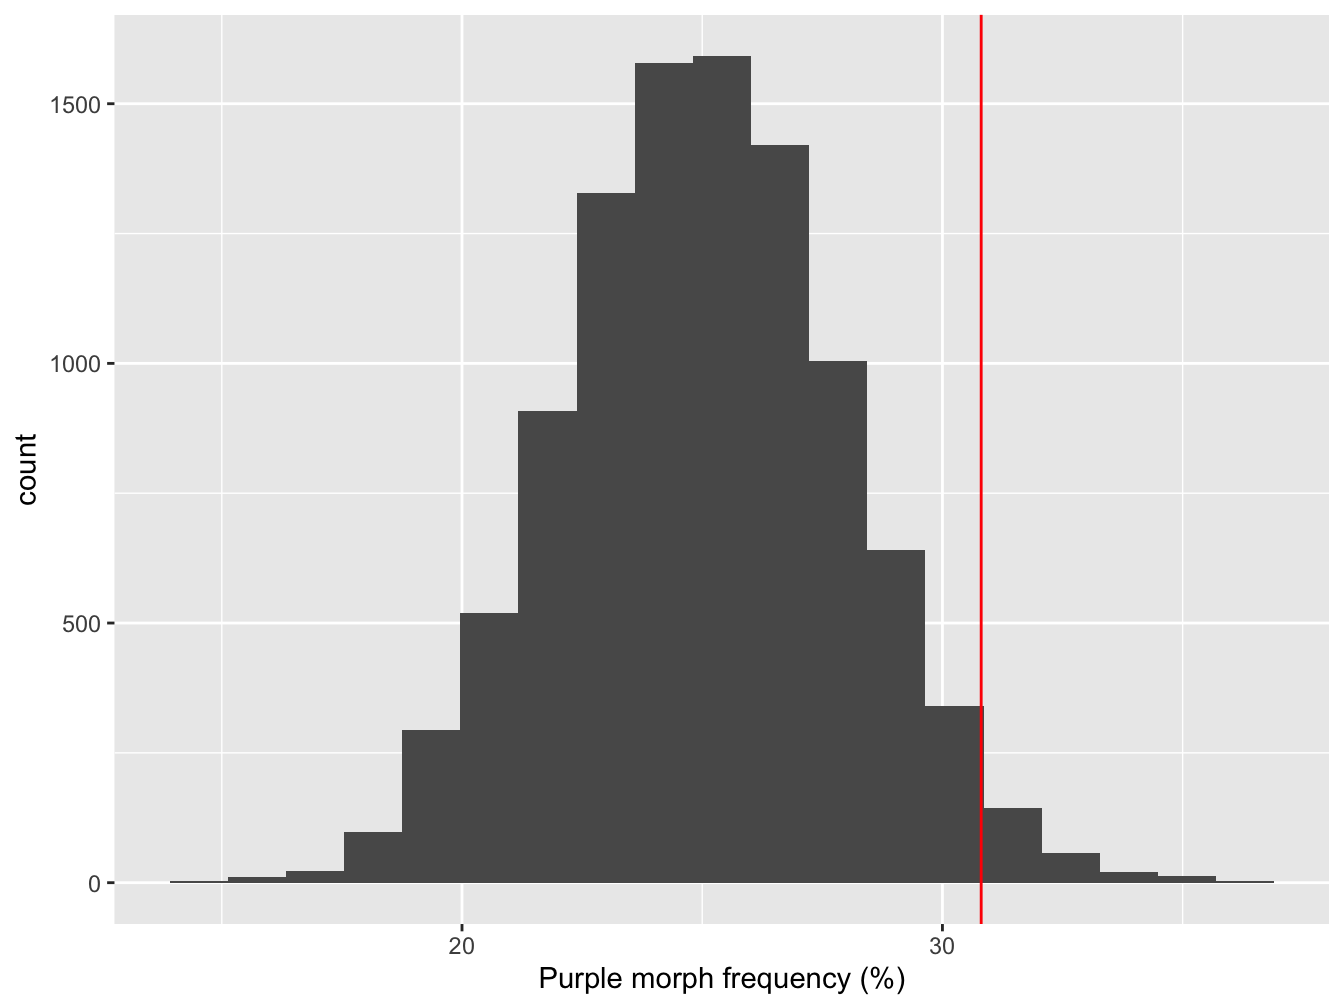
\includegraphics[width=0.75\linewidth]{stats-for-bio_files/figure-latex/boot-samp-dist-25-1} 

}

\caption{Sampling distribution of purple morph frequency under the null hypothesis}\label{fig:boot-samp-dist-25}
\end{figure}

What does this figure tell us? The red line shows where the point
estimate from the true sample lies. It looks like the observed purple
morph frequency would be quite unlikely to have arisen through sampling
variation if the population frequency is 25\%. We can say this because
the observed frequency (red line) lies at the end of one `tail' of the
sampling distribution. We need to be able to make a more precise
statement than this though.

We need to quantify how often the values of the bootstrapped null
distribution are greater than the value we estimated from the sample.
This is easy to do in R:

\begin{Shaded}
\begin{Highlighting}[]
\NormalTok{p_value <-}\StringTok{ }\KeywordTok{sum}\NormalTok{(null_dist >}\StringTok{ }\NormalTok{mean_point_est) /}\StringTok{ }\NormalTok{n_samp}
\NormalTok{p_value}
\end{Highlighting}
\end{Shaded}

\begin{verbatim}
## [1] 0.0265
\end{verbatim}

This number (generally denoted `\emph{p}') is called a
\textbf{\emph{p}-value}. We're going to calculate a lot of
\emph{p}-values in this book. Actually, R will do it for us. We just
have to understand what they mean.

What are we supposed to do with the finding \emph{p} = 0.0265? This is
the probability of obtaining a result equal to, or `more extreme' than,
that which was actually observed, \emph{assuming that the hypothesis
under consideration (the null hypothesis) is true}. The null hypothesis
is one of no effect (or no difference), and so a low \emph{p}-value can
be interpreted as evidence for an effect being present. It's worth
reading that a few times\ldots{}

In our example, it appears that the purple morph frequency we observed
is fairly unlikely to occur if its frequency in the new population
really is 25\%. In biological terms, we take the low \emph{p}-value as
evidence for a difference in purple morph frequency among the
populations. Specifically, it looks like there is support for the
prediction that the purple morph is present at a frequency greater than
25\% in the new study population.

One question remains: How small does a \emph{p}-value have to be before
we are happy to conclude that the effect is probably present? In
practise, we do this by applying a threshold, called a
\textbf{significance level}. If the \emph{p}-value is less than the
chosen significance level we say the result is said to be
\textbf{statistically significant}. Most often (in biology at least), we
use a significance level of \emph{p} \textless{} 0.05 (5\%). Why? The
short answer is that this is just a convention. Nothing more. Really,
there is nothing special about this 5\% threshold other than the fact
that it's the one most often used.

What we just did was to carry out something called a
\textbf{significance test}. It took quite a lot of convoluted reasoning
to get there---we meant it when we said frequentist statistics is odd.
Nonetheless, that rather non-intuitive chain of reasoning, or at least
something similar, underlies all the statistical techniques we use in
this course. The good news is that we don't have to understand the
low-level details to use these tools effectively. We just need to be
able to identify the null hypothesis being used in a particular
significance test and understand how to interpret the associated
\emph{p}-values. These ideas are so important that we'll discuss null
hypotheses and \emph{p}-values a little more in the next two chapters.

\section{Concluding remarks}\label{concluding-remarks}

The bootstrap is a very powerful tool in the right hands, but it is an
advanced technique that can be difficult to apply in complex settings
(e.g.~analysis of experiments). We'll not apply it routinely in this
course. Indeed, you are not expected to be able to use it at all. We
used the technique to help us understand how frequentist ideas are used
to decide if an effect (i.e.~a difference) is really there or not.

The details vary from one problem to the next, but ultimately, if we are
using frequentist ideas we always have to find a way to do the
following\ldots{}

\begin{enumerate}
\def\labelenumi{\arabic{enumi}.}
\item
  assume that there is actually no `effect' (the \textbf{null
  hypothesis}), where an effect is expressed in terms of one or more
  population parameters,
\item
  construct the corresponding \textbf{null distribution} of the
  estimated parameter by working out what would happen if we were to
  take frequent samples in the `no effect' situation,
\end{enumerate}

(Do you see where the word `frequentist' comes from now?)

\begin{enumerate}
\def\labelenumi{\arabic{enumi}.}
\setcounter{enumi}{2}
\tightlist
\item
  and then compare the estimated population parameter to the null
  distribution to arrive at a \textbf{\emph{p}-value}, which evaluates
  how frequently the data would be observed under the hypothesis of no
  effect.
\end{enumerate}

\hypertarget{comparing-populations}{\chapter{Comparing
populations}\label{comparing-populations}}

\section{Making comparisons}\label{making-comparisons}

Scientific inquiry often requires that we evaluate predictions about
`natural' or experimentally induced differences between populations. In
its simplest form this involves just a pair of populations, e.g.

`Do male and female locusts differ in length?'

`Do maize plants photosynthesise at different rates at 25°C and 20°C?'

`Do eagle owls feed on rats of different sizes during winter and
summer?'

`Do purple and green plants differ in their biomass?'

What we're evaluating in this setting is whether or not underlying
\emph{populations} are different in some way. In the previous chapter we
wanted to know whether the purple morph frequency was different from
25\%. In one sense, we were comparing two populations in this study,
because the 25\% number arose from observations of a neighbouring
population. However, that number was also an estimate (though we never
actually said how it was arrived at), which must carry with it some
uncertainty.

In truth, we should have used a methodology that accounts for this
uncertainty to arrive at a more reliable comparison. In order to do
this, we have to step through the same kind of process discussed in the
last few chapters. This chapter demonstrates how to compare two
populations by employing ideas like null hypotheses and \emph{p}-values.
However, the goal is not really to learn how to compare populations
using frequentist techniques. Instead, we want to continue learning how
these ideas are used to construct significance tests and evaluate
predictions. We're also going to introduce something called a `test
statistic'.

First, we need to introduce a new example\ldots{}

\section{A new example}\label{morph-weights-eg}

Let's step through the process introduced in the
\protect\hyperlink{learning-from-data}{Learning from data} chapter. We
want to tackle the following question: ``Is there a fitness difference
between the purple and green morphs in the new population?'' Based on
various observations (that we've already discussed), our hypothesis is
that purple plants are generally fitter than green plants. Since fitness
is often strongly correlated with size in plants, we predict that purple
morphs will be larger. That's our question-hypothesis-prediction sorted
out.

What is (are) the population(s)? Our definition of the population(s) is
different than before. This time we are going to conceive of each morph
as a separate population, i.e.~there are two populations in this new
problem. This change of focus is perfectly valid. Remember, statistical
populations are not really concrete things. That's what we were getting
at when we said statistical populations are defined by the investigator.

What variable should we study? One way to address the prediction of size
differences would be to measure the dry weight biomass of individuals of
each morph. That's a pretty reliable measure of how `big' a plant is.
Dry weight is a numeric variable, measured on a ratio scale (i.e.~zero
really does mean `nothing').

Which population parameter(s) should we work with? Our prediction is
that purple morphs will be larger than green morphs, but what do we
really mean by that? We probably don't mean that every purple plant is
bigger than every green plant. That's a really strong precision, which,
in any case, is not something we could ever validate with a sample.
Instead, we want to know if purple plants are \emph{generally} bigger
than green plants. This can be thought of as a statement about central
tendency, i.e.~we want to evaluate whether purple plants are larger than
green plants, \emph{on average}, in their respective populations. The
population parameters of interest are therefore the mean dry weights of
each morph.

The next step is to gather appropriate samples. Since this is a made-up
example, we'll just cut to the chase. You've already seen the samples
we're going to use. When we read in the `MORPH\_DATA.CSV' in the
previous chapter we found it contained a numeric variable called
\texttt{Weight}. This contains our dry weight biomass information. The
categorical \texttt{Colour} variable analysed in the previous chapter
tells us which kind of colour morph each observation corresponds to.

(These data are
\href{https://cran.r-project.org/web/packages/tidyr/vignettes/tidy-data.html}{tidy}
by the way---each observation is in a separate row and each variable is
in only one column. We only use data in this form in this book.)

\begin{do-something}
You should work through this example from here onward. Read the data
into an R data frame using \texttt{read.csv}, assigning it the name
\texttt{morph.data}. Check it over with \texttt{str} or \texttt{glimpse}
again. Just do it. Yes, you already know about these data, but it is a
good habit to get into.
\end{do-something}

The next step is to calculate point estimates of the mean dry weight of
each morph. These are our `best guesses' of the population means. It may
be useful to know something about the variability of the samples as well
though. We can summarise this with the standard deviation of each sample
(these are not the standard errors!). Here is a reminder of how to do
this using \texttt{dplyr}:

\begin{Shaded}
\begin{Highlighting}[]
\NormalTok{morph.data %>%}\StringTok{ }
\StringTok{  }\KeywordTok{group_by}\NormalTok{(Colour) %>%}\StringTok{ }
\StringTok{  }\KeywordTok{summarise}\NormalTok{(}\DataTypeTok{mean =} \KeywordTok{mean}\NormalTok{(Weight), }
            \DataTypeTok{sd =} \KeywordTok{sd}\NormalTok{(Weight),}
            \DataTypeTok{samp_size =} \KeywordTok{n}\NormalTok{())}
\end{Highlighting}
\end{Shaded}

\begin{verbatim}
## # A tibble: 2 × 4
##   Colour     mean       sd samp_size
##   <fctr>    <dbl>    <dbl>     <int>
## 1  Green 707.8424 149.8092       173
## 2 Purple 766.5638 156.0316        77
\end{verbatim}

This shows that the mean dry weight of the purple morph is greater than
that of green morphs. The standard deviation estimates from the two
samples indicate that the dry weights of purple morphs are more variable
than the green morphs, though this difference isn't very big.

Remember, these numbers are just point estimates derived from limited
samples of the populations. If we sampled the populations again,
sampling variation would result in different estimates. We are not yet
in a position to conclude that purple morphs are bigger than green
morphs.

We'll move onto the main event---evaluating the statistical significance
of the observed difference in means---in the next section. We should
visualise our data first though. We could do this in a variety of ways,
but since we only have two samples, we may as well summarise the full
sample distribution of each morph weight. Here is some \texttt{ggplot2}
code to make a pair of histograms:

\begin{Shaded}
\begin{Highlighting}[]
\KeywordTok{ggplot}\NormalTok{(morph.data, }\KeywordTok{aes}\NormalTok{(}\DataTypeTok{x =} \NormalTok{Weight)) +}\StringTok{ }
\StringTok{  }\KeywordTok{geom_histogram}\NormalTok{(}\DataTypeTok{binwidth =} \DecValTok{50}\NormalTok{) +}\StringTok{ }
\StringTok{  }\KeywordTok{facet_wrap}\NormalTok{(~Colour, }\DataTypeTok{ncol =} \DecValTok{1}\NormalTok{)}
\end{Highlighting}
\end{Shaded}

\begin{figure}

{\centering 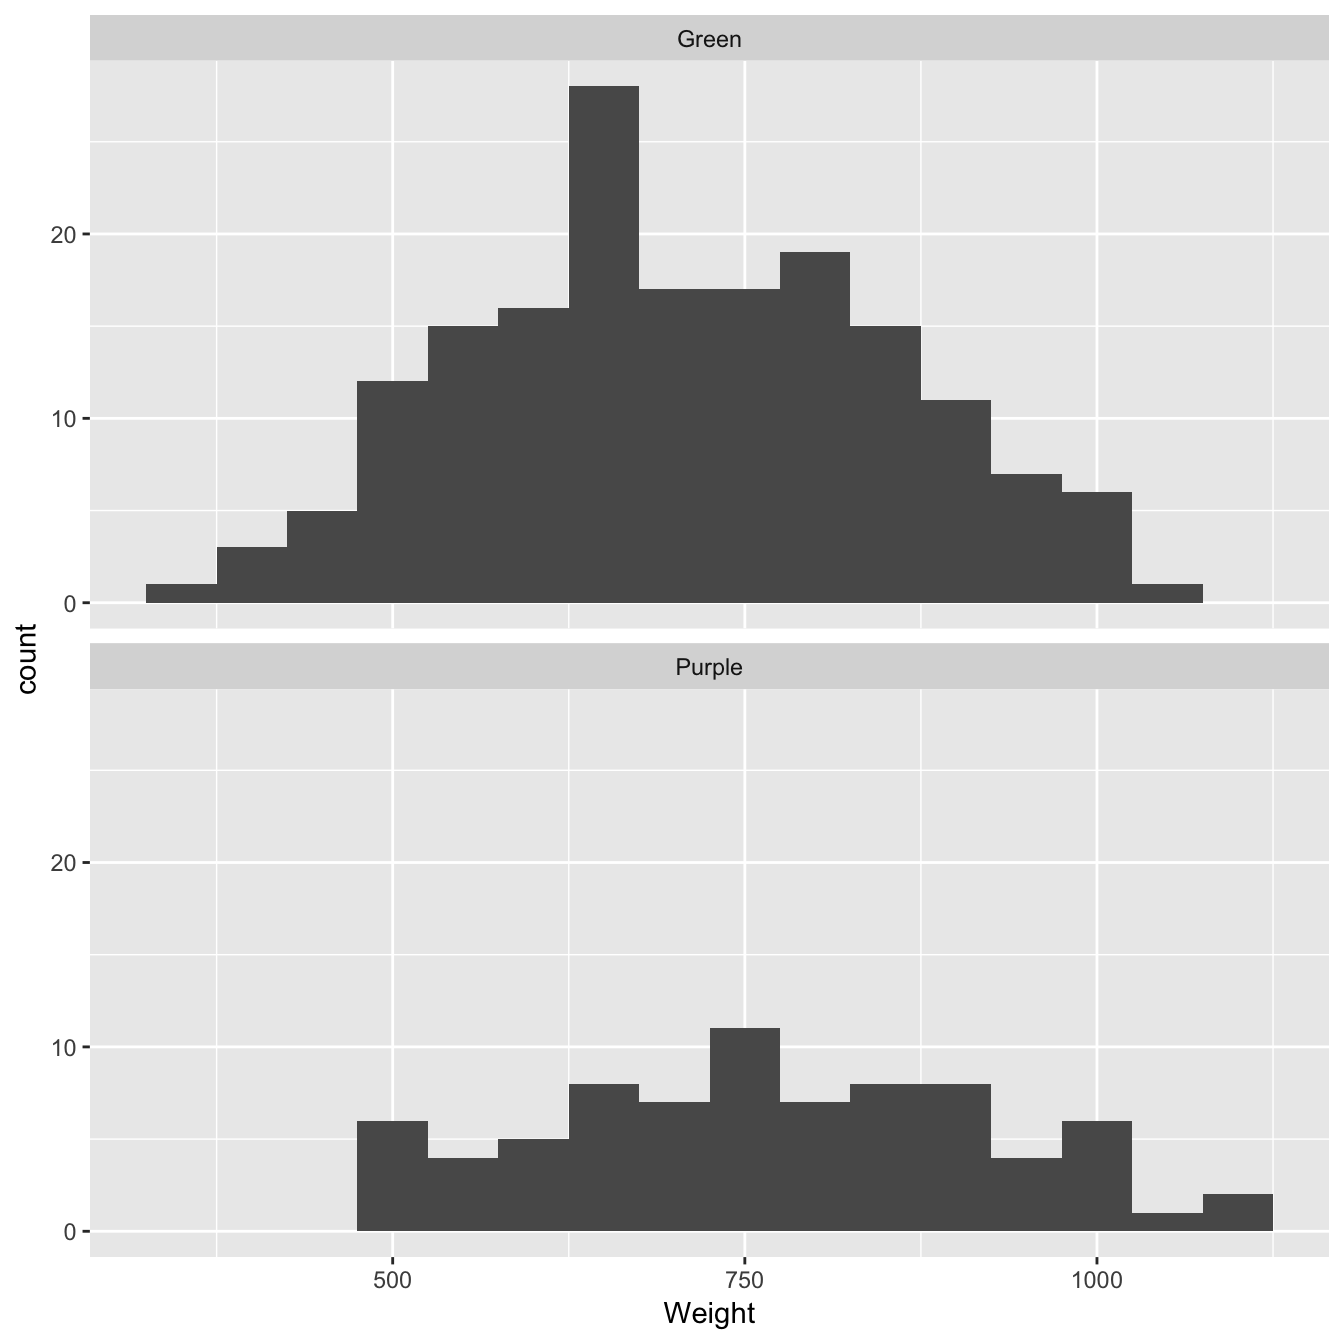
\includegraphics[width=0.6\linewidth]{stats-for-bio_files/figure-latex/two-morph-dist-1} 

}

\caption{Size distributions of purple and green morph samples}\label{fig:two-morph-dist}
\end{figure}

(Hopefully this plot will also remind you how to use the
\texttt{facet\_wrap} function to make a multipanel plot based on the
values of categorical variable---\texttt{Colour} in this instance).

What does this figure tell us? We are interested in the degree of
similarity of the two samples. It looks like purple morph individuals
tend to have higher dry weights than green morphs. Didn't we already
know this? Yes, but that difference could have resulted from the odd
outlier (an unusually large or small value). The histograms indicate
that there really is a general difference in the size of the two morphs.
There is also a lot of overlap between the two dry weight distributions
though, so maybe the difference between the sample means is just a
result of sampling variation.

We need to employ some kind of statistical test\ldots{}

\begin{advanced-box}
\textbf{What do people mean when they `compare samples'?}

By comparing the central tendency (e.g.~the mean) of different samples,
we can evaluate whether or not something we have measured changes, on
average, among different populations. We do this using the information
in the samples to learn about the populations. It's common to use the
phrase `comparing samples' when discussing the statistical tests that
underlie these efforts. This is a little misleading though. When someone
uses a statistical test to `compare samples', what they are really doing
is `using information in the sample to compare population parameters'.
This distinction might seem unnecessarily pedantic (it is a bit, to be
honest). However, it is helpful to keep the right description in mind,
because this helps us remember what a statistical test is really doing.

That said, saying or writing `using information in the sample to compare
population parameters' all the time is dull, so we often revert to the
phrase `comparing samples'. We'll do it in this book sometimes, but try
to keep in mind what we really mean by that phrase.
\end{advanced-box}

\section{Evaluating differences between population
means}\label{evaluating-differences-between-population-means}

We're going to examine one method (there are others) for applying
frequentist concepts to evaluate whether two population means are
different. Specifically, we're going to use something called a
permutation test to evaluate the statistical significance of the
difference between purple and green morph mean dry weights.

In order to assess the strength of evidence for a difference between the
two population means, we have to do something that seems quite strange
(yes, frequentist statistics is odd). We can break this down into four
steps:

\begin{enumerate}
\def\labelenumi{\arabic{enumi}.}
\item
  First, we \emph{assume} there is really no difference between the
  population means. That is, we hypothesise that all the data are
  sampled from a pair of populations that are characterised by a single,
  shared population mean. To put it another way, we pretend there is
  really only one population. You might recognise this trick. It's that
  \textbf{null hypothesis} again.
\item
  Next, we use information in the samples to help us work out what would
  happen if we were to repeatedly take samples in this hypothetical
  situation of `no difference between samples'. We summarise this by
  calculating the null distribution of some kind of \textbf{test
  statistic}.
\end{enumerate}

(We worked directly with the point estimates and their bootstrapped
versions in the previous chapter. When dealing with more complicated
statistical tests, we tend to work with other kinds of numeric
quantities derived from the samples. The generic name for these is `test
statistic'.)

\begin{enumerate}
\def\labelenumi{\arabic{enumi}.}
\setcounter{enumi}{2}
\item
  We then ask, ``if there were no difference between the two groups,
  what is the probability that we would observe a difference that is the
  same as, or more extreme than, the one we actually observed in the
  true sample?'' You may also recognise this probability. It's a
  \textbf{\emph{p}-value}.
\item
  If the observed difference is sufficiently improbable, then we
  conclude that we have found a \textbf{statistically significant}
  result. A statistically significant result is therefore one that is
  inconsistent with the hypothesis of no difference. You might recognise
  this logic from the previous chapter.
\end{enumerate}

There are many different ways to go about realising this process.
Regardless of the details, they all work by trying to evaluate what
happens when we repeatedly sample from a population where the effect of
interest (e.g.~a difference between means) \emph{is absent}.

Let's return to our example to see how this might work in practice.

\section{A permutation test}\label{a-permutation-test}

In our example, a hypothesis of `no difference' between the mean dry
weights of purple and green morphs implies the following: since morphs
are sampled from the same population, the labels `purple' and `green'
are meaningless. These labels don't carry any real information so they
may as well have been randomly assigned to each individual. This
suggests that we can evaluate the statistical significance of the
observed difference as follows:

\begin{enumerate}
\def\labelenumi{\arabic{enumi}.}
\tightlist
\item
  Make a copy of the original sample of purple and green dry weights,
  but do so by randomly assigning the labels `purple' and `green' to
  this new copy of the data. Do this in such a way that the original
  sample sizes are preserved.
\end{enumerate}

(We have to preserve the original sample sizes because we want to mimic
the sampling process that we actually used, i.e.~we want to hold
everything constant apart from the labelling of individuals. The process
of assigning random labels is called permutation.)

\begin{enumerate}
\def\labelenumi{\arabic{enumi}.}
\setcounter{enumi}{1}
\item
  Repeat this permutation scheme until we have a large number of
  artificial samples; 1000-10000 randomly permuted samples may be
  sufficient.
\item
  For each permuted sample, calculate whatever test statistic captures
  the relevant information. In our example, this is the
  \emph{difference} between the mean dry weight of purple and green
  morphs in each sample.
\end{enumerate}

(It doesn't matter which way round we do this. We're going to use
mean(purple) - mean(green) when we do this below.)

\begin{enumerate}
\def\labelenumi{\arabic{enumi}.}
\setcounter{enumi}{3}
\tightlist
\item
  Compare the observed test statistic---the difference between the mean
  dry weights of purple and green plants in the true sample---to the
  distribution of sample statistics from the randomly permuted samples.
\end{enumerate}

This scheme is called a permutation test, because it involves random
permutation of the group labels. Why is it useful? \emph{Each unique
random permutation yields an observation from the null distribution of
the difference among sample means, under the assumption that this
difference is really zero in the population.} We can use this to assess
whether an observed difference is consistent with the hypothesis of no
difference, by looking at where it lies relative to this distribution.

We have implemented a permutation test in R using the purple/green morph
data set for you, using 2500 permutations. We won't show the code
because it uses quite a few new R tricks, and they won't be needed
again. We can look at the first 50 values of the first two permuted
samples to get a sense of how this works:

\begin{verbatim}
##    Purple     Green     Green    Purple     Green     Green     Green 
##  714.3592  693.4924  556.2063  653.6619  672.5207  661.0097  445.1001 
##     Green    Purple     Green    Purple     Green    Purple    Purple 
##  481.5068  647.6679  858.4820  567.4104  597.1629  718.7132  539.8551 
##     Green     Green    Purple     Green     Green     Green     Green 
##  753.0170  807.7700 1085.7036  926.4972  617.1209  632.5897  859.7013 
##    Purple     Green     Green     Green    Purple     Green     Green 
##  815.4634  666.7693  573.5907  694.2877  836.6883  665.8489  617.7895 
##     Green     Green    Purple     Green     Green     Green    Purple 
##  590.5936  775.8980  686.6790  813.4272  506.3904  566.9971  629.5894 
##    Purple     Green     Green     Green    Purple     Green    Purple 
##  878.2477  823.1128  542.7877  507.7345  786.2809  912.5058  853.5730 
##    Purple     Green     Green    Purple     Green    Purple     Green 
##  485.2197  879.7922  852.4711  516.7459  534.4548  702.1948  977.8877 
##     Green 
##  653.5126
\end{verbatim}

\begin{verbatim}
##    Purple    Purple     Green     Green    Purple     Green     Green 
##  714.3592  693.4924  556.2063  653.6619  672.5207  661.0097  445.1001 
##     Green    Purple     Green     Green     Green     Green    Purple 
##  481.5068  647.6679  858.4820  567.4104  597.1629  718.7132  539.8551 
##    Purple    Purple    Purple     Green     Green    Purple     Green 
##  753.0170  807.7700 1085.7036  926.4972  617.1209  632.5897  859.7013 
##    Purple     Green    Purple     Green     Green     Green     Green 
##  815.4634  666.7693  573.5907  694.2877  836.6883  665.8489  617.7895 
##     Green     Green     Green     Green     Green    Purple     Green 
##  590.5936  775.8980  686.6790  813.4272  506.3904  566.9971  629.5894 
##     Green     Green     Green     Green     Green     Green     Green 
##  878.2477  823.1128  542.7877  507.7345  786.2809  912.5058  853.5730 
##     Green     Green     Green     Green     Green     Green     Green 
##  485.2197  879.7922  852.4711  516.7459  534.4548  702.1948  977.8877 
##     Green 
##  653.5126
\end{verbatim}

The data from each permutation are stored as numeric vectors, where each
element of the vector is named according to which morph type it
corresponds to (these are the labels we referred to above). Notice that
the set of numbers doesn't change among the two permuted samples. The
only difference between them is the labelling. The difference between
the mean dry weights in the first permutation is 7.6698902. This
difference is 23.8737542 in the second sample.

What we really care about here is the distribution of these differences.
This distribution is an approximation to the sampling distribution of
the difference between means under the null hypothesis (i.e.~the null
distribution). You may have to read that last sentence a few times. Here
is a histogram that summarises the 2500 mean differences from the
permuted samples:

\begin{figure}

{\centering 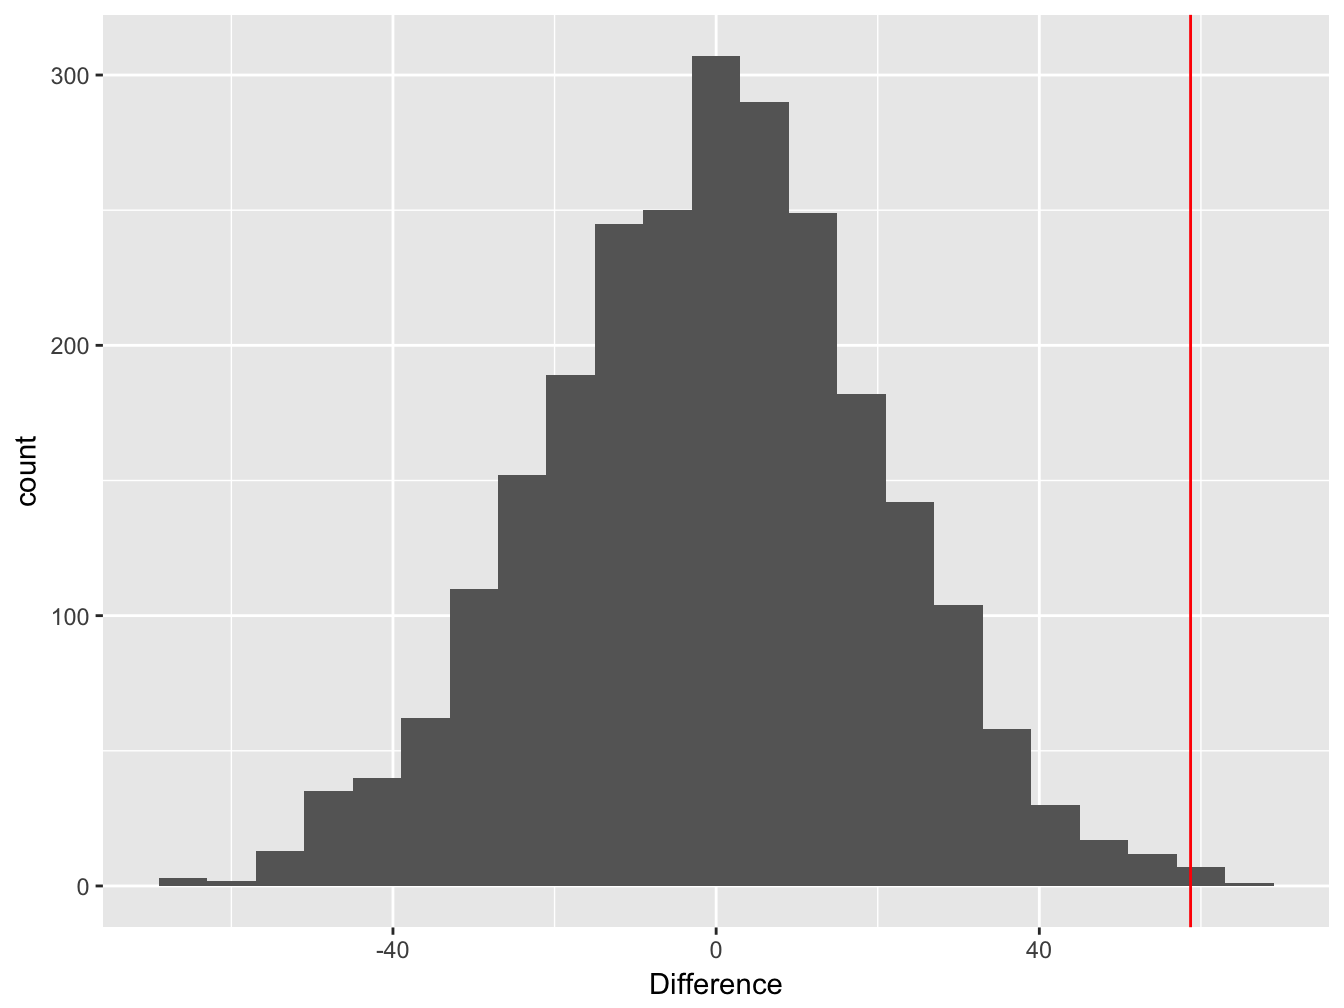
\includegraphics[width=0.8\linewidth]{stats-for-bio_files/figure-latex/permute-dist-1} 

}

\caption{Difference between means of permuted samples}\label{fig:permute-dist}
\end{figure}

Notice that the distribution is centred at zero. This makes sense; if we
take a set of numbers and randomly allocate them to groups, on average,
we expect the difference between the mean of these groups to be zero.

What does the red line show? This is the estimated value of the
difference between the mean purple and green morph dry weights \emph{in
the real sample} (our test statistic). The relevant thing to pay
attention to here is the location of this value within the distribution
of differences. It looks like the estimated difference is very unlikely
to have arisen through sampling variation if the population means of the
two groups were identical. We can say this because the estimated
difference lies at the end of one `tail' of the sampling distribution.

We can quantify the probability of observing the estimated difference
from the null distribution we constructed. Only 4 out of the 2500
permutations ended up being equal to, or `more extreme' (more positive)
than, the observed difference. The probability of finding a difference
in the means equal to or more positive than the observed difference is,
therefore, \emph{p} = 0.0016. This is the \emph{p}-value associated with
our statistical test of significance.

Let's run through the interpretation of that \emph{p}-value. Here's the
general chain of logic again\ldots{} The \emph{p}-value is the
probability of obtaining a test statistic (i.e.~the difference between
means) equal to, or `more extreme' than, the estimated value, assuming
the null hypothesis is true. The null hypothesis is one of no effect
(i.e.~the difference is 0), so a low \emph{p}-value can be interpreted
as evidence for the effect being present. How low does the
\emph{p}-value have to be before we decide we have `enough evidence'? A
significance threshold of \emph{p} \textless{} 0.05 is conventionally
used in biology. If we find \emph{p} \textless{} 0.05, then we conclude
that we found a statistically significant effect.

Here's how this logic applies to our example\ldots{} The permutation
test assumed there was no difference between the purple and green
morphs, so the low \emph{p}-value indicates that the estimated
difference between the mean dry weight of purple and green morphs was
unlikely to have occurred by chance, \emph{if} there is really no
difference at the population level. This means we should interpret the
low \emph{p}-value as evidence for the existence of a difference in mean
dry weight among the populations of purple and green morphs. Since
\emph{p} = 0.0016, we say we found a statistically significant
difference at the 5\% level.

We have to be careful at this point. The test we just did is called a
`one-tailed' test, because we only looked at one end (the tail) of the
null distribution. This kind of test is only appropriate for evaluating
directional predictions (e.g.~purple \textgreater{} green). If, instead
of testing whether purple plants were larger than green plants, we just
wanted to know if they were different (in either direction), we should
have used a `two-tailed' test. These work by looking at both ends of the
null distribution. Don't worry too much if that isn't crystal clear at
the moment. We'll return to idea of one- vs.~two-tailed tests in the
next block of work. For now, it's enough to know that we used a
one-tailed test.

Here's how we might summarise this in a written report:

\begin{quote}
The mean dry weight biomass of purple plants (77) was significantly
greater than that of green plants (173) (one-tailed permutation test,
p\textless{}0.05).
\end{quote}

Notice that we report the sample sizes used, the type of test employed,
and the significance threshold we passed (not the raw \emph{p}-value).

\section{What have we learned?}\label{what-have-we-learned}

Permutation tests are reasonably straightforward to apply in simple
situations, but can be tricky to use in a more complex setting. We are
not expecting you to be able to implement a permutation test yourself.
Just as with bootstrapping in the previous chapter, we used it to
demonstrate how frequentist statistics works. In this instance, for
making comparisons. The basic ideas are no different from those
introduced in the previous chapter\ldots{}

\begin{enumerate}
\def\labelenumi{\arabic{enumi}.}
\item
  define what constitutes an `effect' (e.g.~a difference between means),
  but then assume that there is `no effect' (i.e.~define the
  \textbf{null hypothesis}),
\item
  select an appropriate \textbf{test statistic} that can distinguish
  between the presence of an `effect' and `no effect',
\end{enumerate}

(In practice, each particular kind of statistical test uses a standard
test statistic. We don't have to select these ourselves.)

\begin{enumerate}
\def\labelenumi{\arabic{enumi}.}
\setcounter{enumi}{2}
\item
  construct the corresponding \textbf{null distribution} of the test
  statistic, by working out what would happen if we were to take
  frequent samples in the `no effect' situation,
\item
  and finally, use the null distribution and the test statistic to
  calculate a \textbf{\emph{p}-value}, to evaluate how frequently the
  data would be observed under the hypothesis of no effect.
\end{enumerate}

Notice that we only really introduced one new idea in this chapter. When
evaluating differences among populations we need to work with a single
number that can distinguish between `effect' and `no effect'. This is
called the test statistic. Sometimes this can be expressed in terms of
familiar quantities like means (we just used a difference between means
above), but this isn't always the case. For example, we use something
called an \emph{F}-ratio to evaluate differences among more than two
means. We'll get to this later in the book\ldots{}

\chapter{\texorpdfstring{Hypotheses and
\emph{p}-values}{Hypotheses and p-values}}\label{hypotheses-and-p-values}

\begin{center}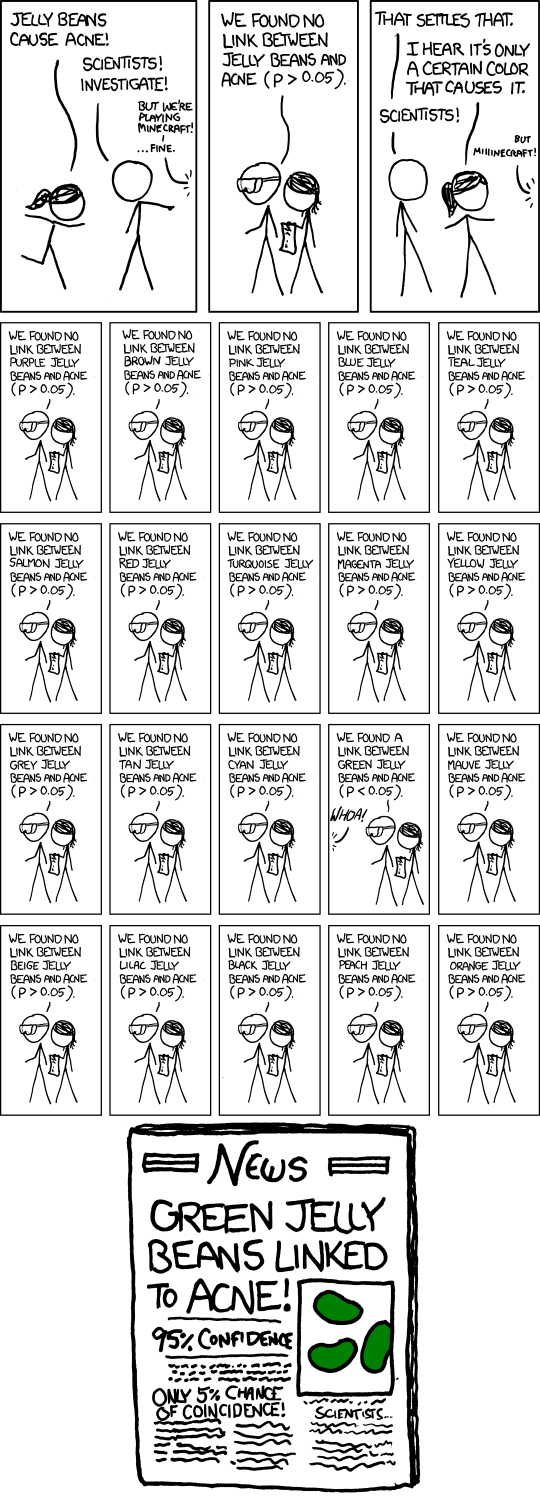
\includegraphics[width=0.6\linewidth]{./images/significant_xkcd} \end{center}

\section{A few words about the null
hypothesis}\label{a-few-words-about-the-null-hypothesis}

When using frequentist statistics we are always asking what would happen
if we continually sampled from a population \emph{where the effect we
are interested in is not present}. This idea of an hypothetical `no
effect' situation is so important that it has a special name; it is
called \textbf{the null hypothesis}. Every kind of statistical test (in
this book at least) works by first specifying a particular null
hypothesis. You can only fully understand the results of a statistical
test if you understand the null hypothesis it relies on.

\subsection{Hypotheses and null
hypotheses}\label{hypotheses-and-null-hypotheses}

When discussing \protect\hyperlink{stages-hypotheses}{the scientific
process}, we have said that an hypothesis is a statement of a proposed
process or mechanism which might be responsible for an observed pattern
or effect. We have also seen that in statistics, we encounter
`hypothesis' used in a different, and quite specific way. In particular
we frequently see the term: \emph{null hypothesis} (often written in
statistics books as H\textsubscript{0}).

The null hypothesis is simply a statement of what we would expect to see
if there is actually no effect of the factor we are looking at (e.g.,
plant morphology) on the variable that we measure (e.g., dry weight
biomass). So in the second plant morph example our null hypothesis was
\emph{There is no difference in mean biomass of purple and green
plants}. All statistical tests you are likely to encounter in biology
work by specifying a null hypothesis and then evaluating the observed
data to see if they deviate from the null hypothesis in a way that is
inconsistent with sampling variation. This may seem like a rather odd
approach, but there are good theoretical and practical reasons for doing
things this way.

You need to be aware of what a null hypothesis is, and what it is used
for, or you won't be able to interpret the results of statistical tests.
However, in general discussion of tests we normally refer to the effect
that is the opposite of the null hypothesis---i.e.~the effect you are
actually interested in---as the \emph{test hypothesis}, or the
\emph{alternative hypothesis} (often denoted H\textsubscript{1} in
statistics books). The alternative hypothesis is essentially a statement
of the effect you are interested in evaluating, e.g., purple and green
plants differ in their mean size. It is a statement of whatever is
implied if the null hypothesis is not true.

Having got all the types of hypothesis sorted out, we can then use a
particular frequentist technique (e.g.~a permutation test) to evaluate
the observed result against that expected if the null hypothesis was
true. The test gives us a probability (\emph{p}-value) telling us how
likely it is that we would have got the result we observe, or a more
extreme result, if the null hypothesis was really true.

If the value is sufficiently small (conventionally if
\emph{p}\textless{}0.05) we judge it unlikely that we would have seen
this result if the null hypothesis was true and consequently we
\emph{reject the null hypothesis} (i.e.~reject the notion that there is
no difference) and instead \emph{accept the alternative hypothesis} that
there is a difference. Note that this is not the same as `proving' the
alternative hypothesis is true. You can't prove anything by collecting
data or carrying out an experiment.

If the probability is large, then it is quite likely that we could have
got the observed result if the null hypothesis was true, i.e.~it is due
to sampling variation. In this case we cannot reject the null
hypothesis. Note that in this situation we say that we ``\emph{do not
reject the null hypothesis}''. This is not the same as accepting that
the null hypothesis is true, paradoxical though this may seem. One
obvious reason for this is that if we only have a small sample then
there may be an effect of the factor we are looking at, but we simply
can't detect it because we don't have enough data.

\section{\texorpdfstring{A few words about
\emph{p}-values}{A few words about p-values}}\label{a-few-words-about-p-values}

It is important to understand the meaning of the probabilities generated
by statistical tests. We have already said a \emph{p}-value is the
proportion of occasions on which you would expect to see a result at
least as extreme as the one you actually observed if the null hypothesis
(of no effect) was true. Conventionally (in biology at least) we accept
a result as statistically significant if \emph{p}\textless{}0.05 (also
expressed as 5\%). There is nothing special about this cut-off point.

A probability of 0.05 is a chance of 1 in 20. This means that if there
really was no effect of the factor we are investigating, we would expect
to get a result significant at \emph{p}=0.05 about 5 times in 100
samples. To envisage it more easily, it is slightly less than the chance
of tossing a coin 4 times and getting 4 heads in a row
(\emph{p}=0.0625). It's not all that rare really. This puts a
`significant' result into context. Would you launch a new drug on the
market or bring a prosecution for pollution on the evidence of the
strength of four heads coming up in a row when a coin is tossed? Well of
course such things are unlikely to hinge on a single test, but it is
always worth bearing in mind what `significance' actually means.

Of course the smaller the probability the more confident one can be that
the effect we see is real. A probability of \emph{p}=0.01 (1 in 100) is
pretty good evidence, and \emph{p}=0.001 (1 in 1000), or less, is better
still. For this reason, in some critical applications such as drug
testing the value set for accepting a result as significant may be lower
(e.g. \emph{p}=0.01). The costs of using a more stringent threshold is
that this increases the possibility of false negatives (called a `type
II' error)--i.e.~we are more likely to fail to detect an effect when it
is really present.

\subsection{\texorpdfstring{What if \emph{p} is close to
0.05?}{What if p is close to 0.05?}}\label{what-if-p-is-close-to-0.05}

The thing to remember here is that, although we tend to use
\emph{p}=0.05 as a cut-off, a \emph{p}-value is really a continuous
measure and \emph{p}=0.055 is not very different from \emph{p}=0.045.
The exact value of \emph{p} will be affected by how well the data
fulfill the assumptions of the test--which will only be approximately
with most biological data, so you shouldn't set too much store by the
difference between \emph{p}=0.045 and \emph{p}=0.055. It would be
irrational on the one hand to reject an idea completely just on the
basis of a result of \emph{p}=0.055, while at the same time being
prepared to invest large amounts of time and money implementing policies
based on a result of \emph{p}=0.045.

\subsection{\texorpdfstring{Presenting
\emph{p}-values}{Presenting p-values}}\label{presenting-p-values}

R will typically display \emph{p}-values from a statistical significance
test to six decimal places (e.g. \emph{p} = 0.003672). Often however,
the results from tests are presented as one of the following four
categories:

\begin{itemize}
\item
  \emph{p} \textgreater{} 0.05, for results which are not statistically
  significant (sometimes also written as `NS'),
\item
  \emph{p} \textless{} 0.05, for results where 0.01 \textless{} \emph{p}
  \textless{} 0.05,
\item
  \emph{p} \textless{} 0.01, for results where 0.001 \textless{}
  \emph{p} \textless{} 0.01,
\item
  \emph{p} \textless{} 0.001 for results where \emph{p} \textless{}
  0.001,
\end{itemize}

Should we use categories for \emph{p}? This style of presentation stems
from the fact that statistical tests often had to be calculated by hand
in the days before everyone had access to a computer. The significance
of the result was difficult to calculate directly, so it would have been
looked up in a special table. These days, a computer can calculate the
exact probability for you, and so there is no particular reason not to
present the results as the actual \emph{p}-value.

It is not wrong to use the four categories above, but giving the actual
probability may be a little more informative to the reader. It could be
useful to know that \emph{p} = 0.014 rather than \emph{p} = 0.047, but
if categories were used both would simply appear as \emph{p} \textless{}
0.05. Similarly it can be informative to know that a test had \emph{p} =
0.06 rather than simply quoting it just as \emph{p} \textgreater{} 0.05
or NS. However, no-one much cares about the difference between very
small probabilities, so if \emph{p} is smaller than 0.001 it can
sensibly be given as simply \emph{p} \textless{} 0.001.

\begin{advanced-box}
\textbf{The asterisks convention}

It is common to see ranges of probabilities coded with asterisks:

\texttt{*} for \emph{p} = 0.05\ldots{}0.01,

\texttt{**} for \emph{p} = 0.01\ldots{}0.001,

\texttt{***} for \emph{p} \textless{} 0.001.

This is common in tables and text in figures as it is a more compact and
visually obvious representation than numbers. However, you should never
use it in the text of a report.
\end{advanced-box}

\section{Biological vs.~statistical
significance}\label{biological-vs.statistical-significance}

A final, but vital, point: do not confuse statistical significance with
biological significance. A result may be statistically highly
significant (say \emph{p} \textless{} 0.001) but biologically trivial.
To give a real example, in a study of the factors determining the
distribution of freshwater invertebrates in a river, the pH of water was
measured in the open water and in the middle of the beds of submerged
vegetation. There was a statistically significant difference in pH
(\emph{p} \textless{} 0.01) but the mean pH values were 7.1 in the open
water and 6.9 in the weeds. This is a very small effect, and almost
certainly of no importance at all to the invertebrates.

The significance of a result depends on a combination of three things
(1) the size of the effect, (2) the variability of the data, (3) the
sample size. Even a tiny effect can be significant if the data have very
little variation and the sample size is large. You should not
automatically equate a significant result with a large effect---you need
to visualise the data\footnote{This is another reason we \emph{always}
  plot our data} , inspect the estimates, and consider the biological
implications of the difference. The statistical results can give you
some guidance in separating genuine differences from random variation,
but they can't tell you whether the difference is biologically
interesting or important---that's your job!

\part{Simple Parametric
Statistics}\label{part-simple-parametric-statistics}
\addcontentsline{toc}{chapter}{(PART) Simple Parametric Statistics}

\part{Evaluating
Associations}\label{part-evaluating-associations}
\addcontentsline{toc}{chapter}{(PART) Evaluating Associations}

\part{Comparing Means}\label{part-comparing-means}


\part{Experimental Design}\label{part-experimental-design}


\part{Miscellaneous Topics}\label{part-miscellaneous-topics}


\appendix
Material}\label{appendix-supplementary-material}
\addcontentsline{toc}{chapter}{(APPENDIX) Supplementary Material}

\chapter{Exercises}\label{exercises}

\section{Week 2}\label{week-2}

\subsection{What kind of variable is
it?}\label{what-kind-of-variable-is-it}

The following table gives a number of measurements taken in the course
of a study of a woodland ecosystem. What type of variable results from
the measurements taken in each case?

\begin{table}

\caption{\label{tab:unnamed-chunk-64}Examples of different kinds of variable.}
\centering
\begin{tabular}[t]{ll}
\toprule
Measurement & Units\\
\midrule
Height of tree & Metres\\
Particulate deposits (pollution) on leaves & Scale of 1 to 5 (very light to very dark)\\
Age of tree & Number of annual rings (one ring formed each year)\\
Month of bud break & Month no. 1 (Jan) - 12 (Dec)\\
Leaf shape & 1 - oval, 2 - lanceolate, 3 - palmate, 4 - pinnate\\
\addlinespace
Number of species of aphid on a tree & Number of spp.\\
Average number of aphids per leaf & Individuals on 20 leaves\\
Time of highest light intensity under leaves & Time of day\\
Occurrence of fungal infection on the leaves & Heavy (>50\% of leaves), Light (<50\% of leaves), Absent (no infection)\\
Tree species & Latin name\\
\addlinespace
Aspect of ground on which each lime tree occurs & Degrees (0-360)\\
Bracken in random quadrats & Visual estimate of \% coverage\\
\bottomrule
\end{tabular}
\end{table}

There are no answers to this question on MOLE. If you're not 100\% sure
what the right answer is in any of these examples, ask a TA or
instructor for help.

\subsection{Definitions}\label{definitions}

The figure below is an attempt to represent some of the concepts you've
been studying this week (e.g.~the sampling distribution, the standard
error, etc):

\begin{figure}

{\centering 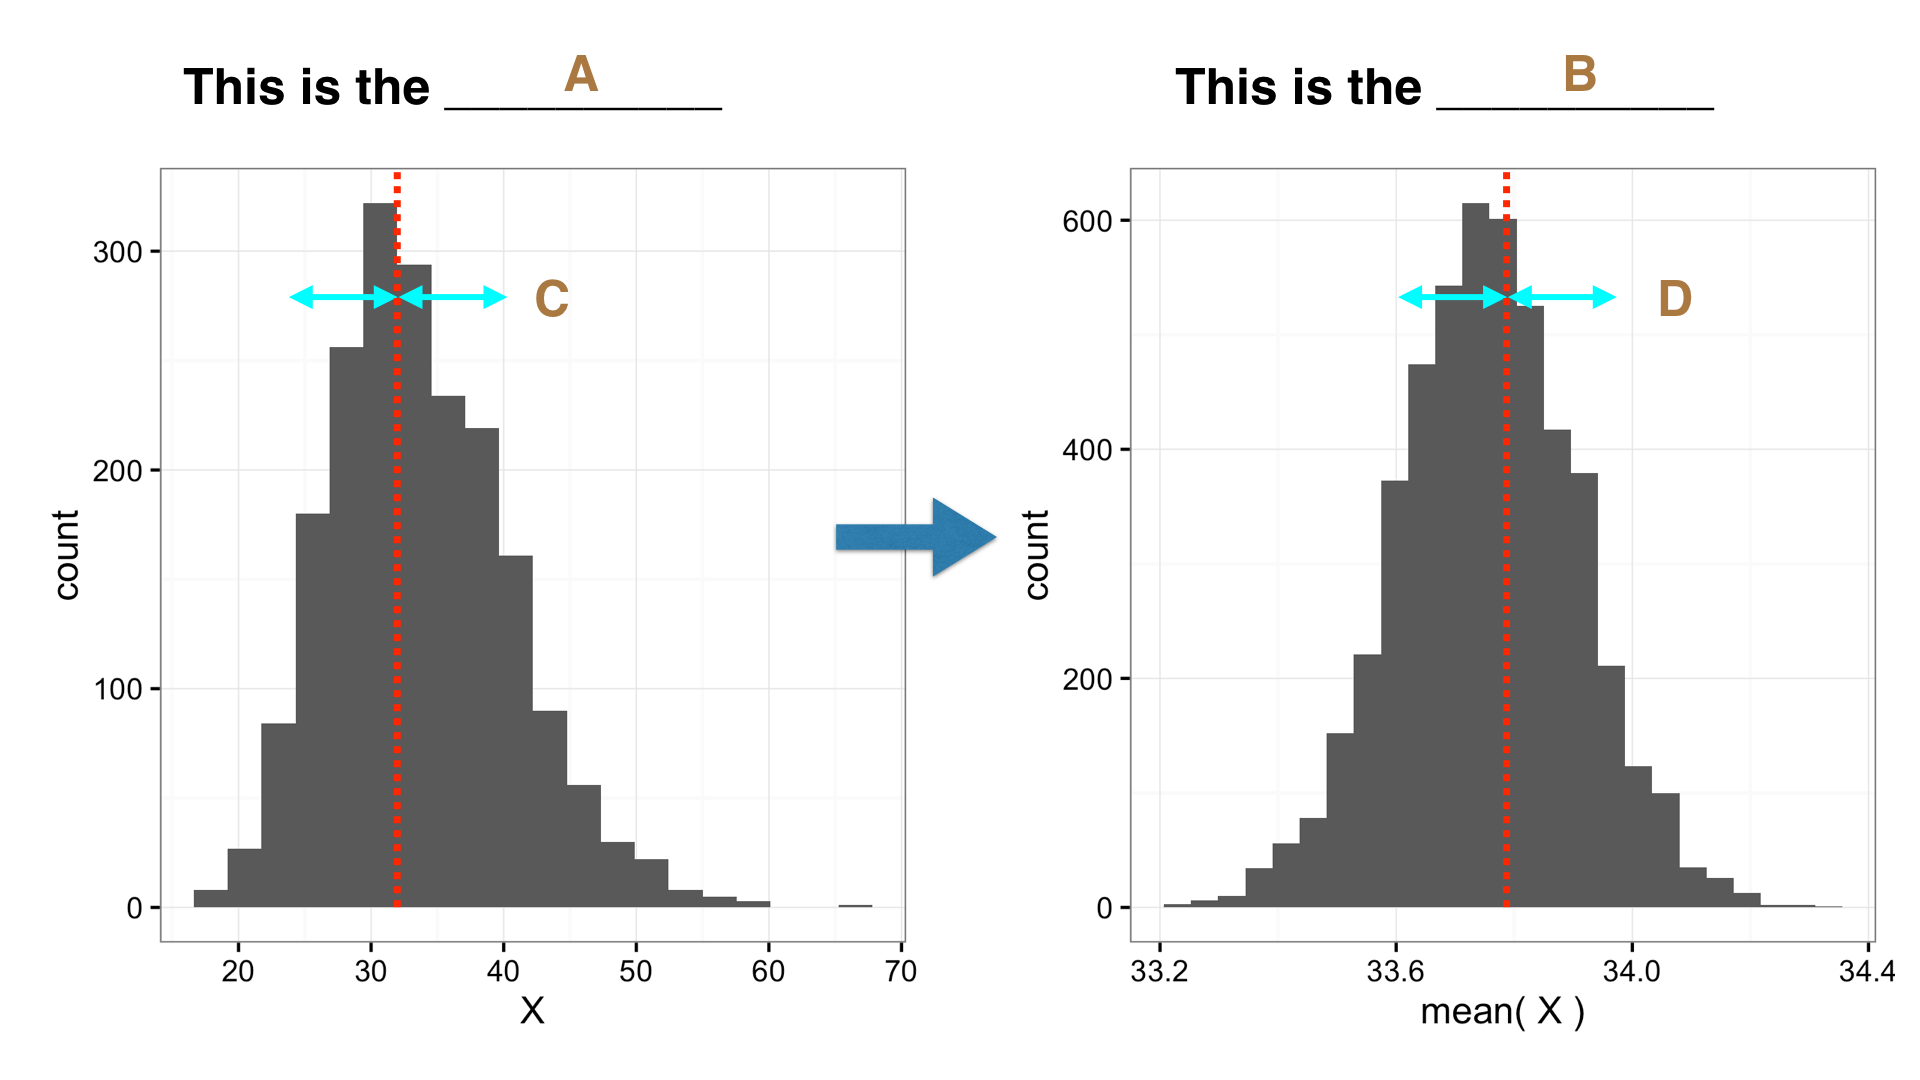
\includegraphics[width=0.8\linewidth]{./images/distro} 

}

\caption{What do the letters refer to?}\label{fig:unnamed-chunk-65}
\end{figure}

\begin{do-something}
\textbf{MOLE Question}

Assign the appropriate term (sampling distribution, standard error, etc)
to the letters A-D in the figure.
\end{do-something}

\subsection{What form do sampling distributions
take?}\label{what-form-do-sampling-distributions-take}

A data file containing a variable sampled from three different
populations (labelled A, B, and C) is available in
SKEWED\_POPULATIONS.CSV. Download the SKEWED\_POPULATIONS.CSV file from
MOLE and place it in your working directory. Read
SKEWED\_POPULATIONS.CSV into an R data frame called \texttt{all\_pops}.
Examine the data set---both visually and in terms of its descriptive
statistics:

\textbf{Inspection.} Use the \texttt{View} function and \textbf{dplyr}
function \texttt{glimpse} (or \texttt{str}) to inspect the `data'. Which
variables are in the data frame? What kind of variables are they
(numeric, categorical, etc)?

\textbf{Descriptive statistics.} Use the appropriate \textbf{dplyr}
functions (\texttt{group\_by} and \texttt{summarise}) to calculate the
mean and standard deviation of the \texttt{Values} variable in each
population. HINT: You will need the \texttt{mean} and
\texttt{sd}functions to help you do this.

\textbf{Graphs.} Use \textbf{ggplot2} to construct three histograms to
summarise the distribution of the variables. HINT: You will need to use
\texttt{geom\_histogram} and the \texttt{facet\_wrap} functions to do
this. Make sure that you use the original data
(\texttt{all\_pops})---not the summarised data.

\begin{do-something}
\textbf{MOLE Question}

How does the distribution of the variable differ across populations in
terms of its central tendency, dispersion and skewness?

In which population is the variable \texttt{Values} the most skewed?
\end{do-something}

Now that you understand a bit about the distribution of the variable in
each population we can move to the next step. You're going to explore
how the shape of a variable's distribution influences the sampling
distribution of its mean. If you're not sure what that last sentence
means, skim over the \protect\hyperlink{sampling-error-1}{Sampling
error} chapter or ask a TA for help before proceeding.

One way to tackle this problem is to work with each population in turn,
using the bootstrapping trick to construct the sampling distribution of
the mean. This involves three steps. First we have to extract the subset
of values we require and store these in a numeric vector (step 1). Then
we use a bit of R trickery to calculate 1000 bootstrapped means (step
2), and finally, parcel up the result into a data frame (step 3). Here's
how this works for variable A:

\begin{Shaded}
\begin{Highlighting}[]
\CommentTok{# 1. extract the values of the variable}
\NormalTok{x <-}\StringTok{ }\KeywordTok{filter}\NormalTok{(all_pops, Population ==}\StringTok{ "A"}\NormalTok{)$Values}
\CommentTok{# 2. carry out the bootstrapping (you don't need to understand this)}
\NormalTok{boot_means <-}\StringTok{ }\KeywordTok{replicate}\NormalTok{(}\DecValTok{1000}\NormalTok{, }\KeywordTok{mean}\NormalTok{(}\KeywordTok{sample}\NormalTok{(x, }\DataTypeTok{size =} \DecValTok{25}\NormalTok{, }\DataTypeTok{replace =} \OtherTok{TRUE}\NormalTok{)))}
\CommentTok{# 3. wrap up the result as a data frame}
\NormalTok{plot_df <-}\StringTok{ }\KeywordTok{data.frame}\NormalTok{(boot_means)}
\end{Highlighting}
\end{Shaded}

Note that this code creates bootstrapped samples of 25 observations to
construct the sampling distributions in the exercise above
(\texttt{size\ =\ 25}).

Once we have the bootstrapped sampling distribution of the mean we need
to visualise this as a histogram. You should be able to work out how to
do this using \textbf{ggplot2}. Construct this histogram for each of the
variables. Just look at each histogram in turn. There's no need to try
to make one plot containing all three histograms. Look at each one
carefully, paying close attention to the form of the original sample and
the bootstrapped sampling distribution of their mean.

\begin{do-something}
\textbf{MOLE Question}

Are the sampling distributions of the means more, or less, skewed than
the distribution of the corresponding variables?

Which variable (A, B, or C) has the most skewed sampling distribution
associated with its mean?
\end{do-something}

You used bootstrapped samples of 25 observations to construct the
sampling distributions in the exercise above (\texttt{size\ =\ 25}). You
can change this number by altering the \texttt{size} argument of the
\texttt{sample} function. Use this fact to explore how the shape of the
sampling distribution changes as you increase sample size of the `C'
variable. Start by using only 10 individuals in each bootstrapped
sample, and gradually increase this to 100.

\begin{do-something}
\textbf{MOLE Question}

What happens to the shape of the sampling distribution of the mean of
the `C' variable as you change the bootstrapped sample size?
\end{do-something}

\subsection{How does sample size influence the standard
error?}\label{how-does-sample-size-influence-the-standard-error}

Think back to the plant colour morph example. We used a simulation in R
to calculate the approximate sampling distribution of purple morph
frequency estimates. We used this to examine how the amount of sampling
variation changes with sample size. We noted that, in general, it seems
to decline with sample size. The bigger our sample, the more precise our
estimate. That might seem obvious, but what form does this relationship
take?

We've written an R function to allow you to explore how the size of
samples influence the standard error of purple morph frequency
estimates. You can read this into R by running the following line of R
code (just copy and paste it into the Console):

\begin{Shaded}
\begin{Highlighting}[]
\NormalTok{sample_plants <-}\StringTok{ }\NormalTok{function(samp_sizes, prob) \{}
  \KeywordTok{sapply}\NormalTok{(samp_sizes, function (size) \{}
    \NormalTok{raw_samples <-}\StringTok{ }\KeywordTok{rbinom}\NormalTok{(}\DataTypeTok{n =} \DecValTok{10000}\NormalTok{, }\DataTypeTok{size =} \NormalTok{size, }\DataTypeTok{prob =} \NormalTok{prob)}
    \KeywordTok{sd}\NormalTok{(}\DecValTok{100} \NormalTok{*}\StringTok{ }\NormalTok{raw_samples /}\StringTok{ }\NormalTok{size)}
  \NormalTok{\})}
\NormalTok{\}}
\end{Highlighting}
\end{Shaded}

(You are not expected to understand how this works!)

This will create a function called \texttt{sample\_plants} that's ready
for you to use. Here's how it works:

\begin{Shaded}
\begin{Highlighting}[]
\KeywordTok{sample_plants}\NormalTok{(}\DataTypeTok{samp_sizes =} \KeywordTok{c}\NormalTok{(}\DecValTok{10}\NormalTok{, }\DecValTok{20}\NormalTok{, }\DecValTok{40}\NormalTok{, }\DecValTok{100}\NormalTok{), }\DataTypeTok{prob =} \FloatTok{0.4}\NormalTok{)}
\end{Highlighting}
\end{Shaded}

\begin{verbatim}
## [1] 15.470698 10.987846  7.696500  4.899136
\end{verbatim}

The first argument, \texttt{samp\_sizes\ =\ c(10,\ 20,\ 40,\ 100)},
provides the set of sample sizes we want the standard errors for, the
second argument, \texttt{prob\ =\ 0.4}, is the frequency of purple
plants (expressed as a probability) in the population. The function
returns a vector of numbers that are the standard errors at each sample
size.

The easiest way to explore the relationship between sample size and
standard error is to simply plot it. Since we use \textbf{ggplot2}, we
need to collect together the inputs and outputs of these simulations
into a data frame. Here's one way to do this:

\begin{Shaded}
\begin{Highlighting}[]
\NormalTok{sim_data <-}\StringTok{ }
\StringTok{  }\KeywordTok{data.frame}\NormalTok{(}\DataTypeTok{sample_size =} \KeywordTok{c}\NormalTok{(}\DecValTok{10}\NormalTok{, }\DecValTok{20}\NormalTok{, }\DecValTok{40}\NormalTok{, }\DecValTok{100}\NormalTok{)) %>%}\StringTok{ }
\StringTok{  }\KeywordTok{mutate}\NormalTok{(}\DataTypeTok{se =} \KeywordTok{sample_plants}\NormalTok{(sample_size, }\DataTypeTok{prob =} \FloatTok{0.4}\NormalTok{))}
\NormalTok{sim_data}
\end{Highlighting}
\end{Shaded}

\begin{verbatim}
##   sample_size        se
## 1          10 15.649418
## 2          20 10.844418
## 3          40  7.678895
## 4         100  4.877646
\end{verbatim}

Use the above code to vary the sample size from around 20 to 500 (the
exact numbers don't matter too much), assuming that the purple morph
frequency is 0.4 (\texttt{prob\ =\ 0.4}). You only need to vary the
values assigned to \texttt{sample.size} to do this. Make a plot to
investigate how the standard error changes as the sample size increases.

\begin{do-something}
\textbf{MOLE Question}

Does the standard error halve when you double the sample size, or is the
relationship more complicated? If you think the relationship is more
complicated, what form does it take?
\end{do-something}

Now repeat the exercise with assuming that the purple morph frequency is
0.1 (\texttt{prob\ =\ 0.1}).

\begin{do-something}
\textbf{MOLE Question}

Does the standard error depend on purple morph frequency? Does it get
smaller or larger when we move from a frequency of 0.4 to 0.1?
\end{do-something}

\section{Week 3}\label{week-3}

\subsection{Sample size and statistical
power}\label{sample-size-and-statistical-power}

The TWO\_POPS\_1.CSV file contains values of a numeric variable in two
different populations (labelled A and B). The file contains a large
sample from each of the two populations. For the purpose of this
exercise you'll treat each these as though they are the `whole
population' (even though they are really just limited samples). Download
the TWO\_POPS\_1.CSV file from MOLE and place it in your working
directory, then read this into an R data frame called
\texttt{pop\_info\_1}.

Examine the populations---both in terms of their descriptive statistics,
and visually:

\textbf{Inspection.} Use the \texttt{View} function and \textbf{dplyr}
function \texttt{glimpse} (or \texttt{str}) to inspect the `data'. Which
variables are in the data frame? What kind of variables are they
(numeric, categorical, etc)?

\textbf{Descriptive statistics.} Use the appropriate \textbf{dplyr}
functions (\texttt{group\_by} and \texttt{summarise}) to calculate the
mean, standard deviation and sample size of \texttt{Values} in each
population.

\textbf{Graphs.} Use \textbf{ggplot2} to construct a pair of histograms
to summarise the distribution of the variable in each population. This
is most easily done using \texttt{facet\_wrap}.

\begin{do-something}
\textbf{MOLE Question}

Note down the key features of the distribution of the variable in each
population. Does the variable seem to be normally distributed? How do
the distributions differ in terms of their central tendency and
dispersion among the two populations?
\end{do-something}

Now that you understand the two populations a little bit we can start to
experiment with them. We want you to explore what happens when you draw
different sized samples from these two populations. Specifically, you're
going to explore how the sample size influences your ability to detect a
difference in the population means, using a permutation test. To start
with, you'll use \textbf{dplyr} to simulate the process of drawing an
equal sized sample from each population:

\begin{Shaded}
\begin{Highlighting}[]
\CommentTok{# take a sample from each population}
\NormalTok{use_data <-}\StringTok{ }\NormalTok{pop_info_1 %>%}\StringTok{ }
\StringTok{  }\KeywordTok{group_by}\NormalTok{(Population) %>%}\StringTok{ }
\StringTok{  }\KeywordTok{sample_n}\NormalTok{(}\DecValTok{10}\NormalTok{) %>%}\StringTok{ }
\StringTok{  }\NormalTok{ungroup}
\end{Highlighting}
\end{Shaded}

Copy this first chunk of \textbf{dplyr} code into your script and run
it. After doing this, \texttt{use\_data} will contain a sample of 10
observations from each population (use \texttt{View} to verify this).
You haven't seen it before, but the \texttt{sample\_n} function just
takes a sample from a data frame, i.e. \texttt{sample\_n(10)} takes a
sample of 10 observations. Using it with \texttt{group\_by} just takes a
sample from each population. The \texttt{ungroup} bit at the end removes
the grouping information from the output. The next bit won't work
properly if you forget this.

Now that you have a sample to work with, you need to use a statistical
test to assess the evidence for whether or not the population means are
different. You should already know the answer to this question from your
initial explorations (go back to these again if you're not sure). You'll
use a permutation test to do this. You should skim back over the
\protect\hyperlink{comparing-populations}{Comparing populations} chapter
if you're not sure how this works, or ask a TA to remind you.

Here is some not-at-all-simple R code that performs the permutation
test:

\begin{Shaded}
\begin{Highlighting}[]
\CommentTok{# permutation test (difficult R code!)}
\NormalTok{plt_info <-}\StringTok{ }\KeywordTok{replicate}\NormalTok{(}\DecValTok{1000}\NormalTok{, }\DataTypeTok{simplify =} \OtherTok{TRUE}\NormalTok{, \{}
  \NormalTok{use_data %>%}\StringTok{ }
\StringTok{    }\KeywordTok{mutate}\NormalTok{(}\DataTypeTok{Values =} \KeywordTok{sample}\NormalTok{(Values)) %>%}\StringTok{ }
\StringTok{    }\KeywordTok{group_by}\NormalTok{(Population) %>%}\StringTok{ }
\StringTok{    }\KeywordTok{summarise}\NormalTok{(}\DataTypeTok{X =} \KeywordTok{mean}\NormalTok{(Values)) %>%}\StringTok{ }
\StringTok{    `}\DataTypeTok{$}\StringTok{`}\NormalTok{(X) %>%}\StringTok{ }\NormalTok{diff}
\NormalTok{\}) %>%}\StringTok{ }\KeywordTok{data.frame}\NormalTok{(}\DataTypeTok{diff_means =} \NormalTok{.)}
\end{Highlighting}
\end{Shaded}

There are quite a few tricks used in that R code. And yes, you are not
expected to understand how it all works. Ask a TA for an explanation if
you're curious though. You just need to use it, so copy this next chunk
of code into your script.

Finally, here is some R code that plots the resulting null distribution
of the difference between means, along with the difference actually
observed in the sample (red line):

\begin{Shaded}
\begin{Highlighting}[]
\CommentTok{# compute the difference between (more tricky code)}
\NormalTok{mean_diff <-}\StringTok{ }\NormalTok{use_data %>%}\StringTok{ }
\StringTok{  }\KeywordTok{group_by}\NormalTok{(Population) %>%}\StringTok{ }
\StringTok{  }\KeywordTok{summarise}\NormalTok{(}\DataTypeTok{X =} \KeywordTok{mean}\NormalTok{(Values)) %>%}\StringTok{ `}\DataTypeTok{$}\StringTok{`}\NormalTok{(X) %>%}\StringTok{ }\NormalTok{diff}
\CommentTok{# plot everything (this bit should make sense to you)}
\KeywordTok{ggplot}\NormalTok{(plt_info, }\KeywordTok{aes}\NormalTok{(}\DataTypeTok{x =} \NormalTok{diff_means)) +}\StringTok{ }
\StringTok{  }\KeywordTok{geom_histogram}\NormalTok{(}\DataTypeTok{bins =} \DecValTok{18}\NormalTok{) +}
\StringTok{  }\KeywordTok{geom_vline}\NormalTok{(}\DataTypeTok{xintercept =} \NormalTok{mean_diff, }\DataTypeTok{colour =} \StringTok{"red"}\NormalTok{)}
\end{Highlighting}
\end{Shaded}

Copy this last chunk of code into your script. You should now have a
script that contains all three chunks of code, in the correct order. If
everything is working you should end up with a picture like this one:
\includegraphics{stats-for-bio_files/figure-latex/unnamed-chunk-85-1.pdf}
Yours won't be the same, as you will have used a different sample.

Here's what we want you to do with this\ldots{} Using a sample size of
10 (i.e.~leave \texttt{sample\_n(10)} as it is), run all three chunks
several times, checking the final plot each time before you run them
again. About 10-20 runs should be enough to answer the first
question\ldots{}

\begin{do-something}
\textbf{MOLE Question}

Is a sample size of 10 sufficient to detect a difference between the
population means? Make sure you can explain your answer.
\end{do-something}

Now repeat this exercise, using successively larger sample sizes,
e.g.~10, 20, 40, 80, and 160. To use a sample size of 20 you would
change \texttt{sample\_n(10)} to \texttt{sample\_n(20)}. That's
all---there's no need to make a new copy of all the code (it will end up
as a big mess if you do this). Just change the \texttt{sample\_n} part
and run the new version of everything several times. You might need to
experiment a bit with the sample sizes, but don;t make them much bigger
than about 200.

\begin{do-something}
\textbf{MOLE Question}

Which sample size seems to be sufficient to detect a difference between
the population means?
\end{do-something}

\subsection{A bit more about statistical
power}\label{a-bit-more-about-statistical-power}

That last exercise was all about statistical power. The statistical
power of a test relates to its ability to detect an effect when it is
present. You just explored how sample size affects the power of a test.
In this next exercise you are going to investigate how other features of
samples affect the statistical power of a test. You'll do this by
repeating the last exercise using two new pairs of populations.

The information about the two new population pairs are contained in the
TWO\_POPS\_2.CSV and TWO\_POPS\_3.CSV files (these have the same
structure as TWO\_POPS\_1.CSV). Download the two files from MOLE and
place them in your working directory, then read them into an R data
frames called \texttt{pop\_info\_2} and \texttt{pop\_info\_3},
respectively. Make sure you place the R code that does this near the top
of your script so that it occurs \emph{before} all the code that
performs the permutation test.

Repeat the \textbf{Descriptive statistics} and \textbf{Graphs} steps
from the previous exercise to make sure you understand these new
population pairs. Again, make sure you place the R code that does this
\emph{before} all the code that performs the permutation test (but after
the reading-in-data step).

\begin{do-something}
\textbf{MOLE Question}

Note down the key features of the distributions of each pair of
populations. Note their central tendency and dispersion. How do the new
pairs differ from the population pair used in the previous exercise?
\end{do-something}

Now, for each population pair in turn, repeat the previous exercise
where you varied the sample size. The only part of the permutation test
and plotting code you need to alter is the first chunk. For example, to
use sample sizes of 40 from the second population pair (in
\texttt{pop\_info\_2}) you would use:

\begin{Shaded}
\begin{Highlighting}[]
\CommentTok{# take a sample from each population}
\NormalTok{use_data <-}\StringTok{ }\NormalTok{pop_info_2 %>%}\StringTok{ }
\StringTok{  }\KeywordTok{group_by}\NormalTok{(Population) %>%}\StringTok{ }
\StringTok{  }\KeywordTok{sample_n}\NormalTok{(}\DecValTok{40}\NormalTok{) %>%}\StringTok{ }
\StringTok{  }\NormalTok{ungroup}
\end{Highlighting}
\end{Shaded}

The aim of this exercise is to see how big the samples have to get
before you think you can reliably detect a difference in the means using
the permutation test. The ultimate goal is to understand how the
distributions of the population pairs influence your ability to detect
the difference in their means.

\begin{do-something}
\textbf{MOLE Question}

Think about the differences between three population pairs. Which aspect
(or aspects) of their distributions do you think best explains the
change in the statistical power of the permutation test you've been
using?
\end{do-something}

\bibliography{packages.bib,book.bib}


\end{document}
